\documentclass[11pt, oneside]{book}
\usepackage[paperwidth=17cm, paperheight=22.5cm, bottom=2.5cm, right=2.5cm]{geometry}
\usepackage[utf8]{inputenc}
\usepackage[english]{babel}
\usepackage{amssymb,amsmath,amsthm,amsfonts,mathtools}
\usepackage{tikz}
\usetikzlibrary{arrows.meta, positioning}
\usepackage{chngcntr}
\counterwithin{figure}{chapter}
\usepackage{tcolorbox}
\usepackage{microtype}
\usepackage{listings}
\lstdefinestyle{Rstyle}{
  language=R,
  basicstyle=\ttfamily\footnotesize,
  keywordstyle=\color{black},
  commentstyle=\color{miAzul},
  stringstyle=\color{miVerde},
  backgroundcolor=\color{gray!5},
  frame=lines,
  rulecolor=\color{black},
  breaklines=true,
  captionpos=b,
  showstringspaces=false
}

% Para eliminar guiones y justificar texto
\tolerance=1
\emergencystretch=\maxdimen
\hyphenpenalty=10000
\hbadness=10000

\linespread{1.25} % Asemeja el interlineado 1.5 de Word

\let\oldfootnote\footnote % Deja espacio entre el número del pie de página y el inicio del texto
\renewcommand\footnote[1]{%
\oldfootnote{\hspace{0.05mm}#1}}

\renewcommand{\thefootnote} {\textcolor{miVerde}{\arabic{footnote}}} % Súperindice a color negro

\setlength{\footnotesep}{0.75\baselineskip}
\setlength{\parskip}{1em}
\setlength{\parindent}{0pt}

% ---- LINKS ----
\usepackage{hyperref}
\hypersetup{colorlinks=true, urlcolor=miRojo, citecolor=miAzul, linkcolor=miVerde}

% ---- IMÁGENES ----
\usepackage{graphicx}
\graphicspath{{../../plots/}{../../imgs/}{plots/}{imgs/}}
\newcommand{\thesislogopath}{../../logo-ITAM.png}
\IfFileExists{../../logo-ITAM.png}{}{\renewcommand{\thesislogopath}{logo-ITAM.png}}
\newcommand{\thesisbib}{../../biblo}
\IfFileExists{../../biblo.bib}{}{\renewcommand{\thesisbib}{biblo}}
\newcommand{\rlogopath}{../../plots/Rlogo.png}
\IfFileExists{../../plots/Rlogo.png}{}{\renewcommand{\rlogopath}{plots/Rlogo.png}}

% ---- FORMATO DE TÍTULOS ----
\usepackage{titlesec}
\titlespacing{\section}{0pt}{1em plus 4pt minus 2pt}{0pt plus 2pt minus 2pt}
\titlespacing{\subsection}{0pt}{1em plus 4pt minus 2pt}{0pt plus 2pt minus 2pt}
\titlespacing{\subsubsection}{0pt}{1em plus 4pt minus 2pt}{0pt plus 2pt minus 2pt}

% ---- FORMATO DE LISTAS ----
\usepackage{enumitem}
\setlist[itemize]{topsep=-0.5em} % es media m para compensar
\setlist[enumerate]{topsep=-0.5em}



% ---- COLORES ----
\usepackage{xcolor}
\definecolor{miAzul}{RGB}{13, 33, 161}
\definecolor{miRojo}{RGB}{186, 24, 27}
\definecolor{miVerde}{RGB}{65, 123, 90}
\definecolor{LightGray}{gray}{0.95}
\definecolor{codegray}{gray}{0.9}

% ---- BIBLIOGRAFÍA ----
\usepackage{apacite}
\bibliographystyle{apacite}
\usepackage{etoolbox}
\apptocmd{\thebibliography}{\setlength{\itemsep}{6pt}\interlinepenalty=10000}{}{}

% ---- FORMATO DE LAS PÁGINAS ----
%\usepackage[a4paper, width=165mm, top=20mm, bottom = 20mm]{geometry}

\setlength{\headheight}{15pt}

\setlength{\parskip}{1em}
\setlength{\parindent}{0cm}


% ---- CAJAS DE COLORES ----
\usepackage{tcolorbox}
\usepackage{bm}
\usepackage{booktabs}
\usepackage{colortbl}
\usepackage{longtable}
\usepackage{float}
\usepackage{caption}
\captionsetup{justification=centerlast, singlelinecheck=true}

\title{
    Thesis \\
    \large \textbf{Draft}
}
\author{
Fernando Pérez Millán, 189380}
\date{-}

\newcommand\TEI{\mathrel{\overset{\makebox[0pt]{\mbox{\normalfont\tiny\sffamily TEI}}}{=}}}
\newcommand\IND{\mathrel{\overset{\makebox[0pt]{\mbox{\normalfont\tiny\sffamily ind}}}{=}}}
\DeclareMathOperator{\var}{var}
\DeclareMathOperator{\diag}{diag}
\DeclareMathOperator{\vas}{v.a.}
\DeclareMathOperator{\ee}{ee}
\DeclareMathOperator{\I}{I}
\renewcommand{\P}{\mathbb{P}}
\newcommand{\E}{\mathbb{E}}
\newcommand{\R}{\mathbb{R}}

\numberwithin{equation}{chapter}
\numberwithin{table}{chapter}

\newcommand{\Rlogo}{\protect\includegraphics[height=1.8ex,keepaspectratio]{\rlogopath}}

% --- Páginas a la derecha (impresión a doble cara) ---
% Contamos las páginas FÍSICAS realmente impresas (inmune a los reinicios
% de numeración de \frontmatter y \mainmatter) y redefinimos
% \cleardoublepage para que el contenido siguiente caiga siempre en una
% página derecha (recto), insertando una página en blanco sólo si hace
% falta. Como \chapter, \frontmatter, \tableofcontents y \mainmatter
% llaman a \cleardoublepage, cada sección y capítulo arranca a la derecha.
\usepackage{atbegshi}
\newcounter{physpage}
\AtBeginShipout{\stepcounter{physpage}}
\renewcommand{\cleardoublepage}{%
  \clearpage
  \ifodd\value{physpage}%
    \thispagestyle{empty}\mbox{}\clearpage
  \fi
}

\begin{document}

\pagestyle{plain}
\frontmatter

%----------------------------------------------------------------------------------------
%	EXECUTIVE SUMMARY
%----------------------------------------------------------------------------------------
\chapter*{Executive Summary}

{\small\textit{This document opens with an executive summary of the thesis. The complete manuscript that follows—starting from the cover page—is reproduced in full and without modification.}}

\section*{Objective}

The objective of this thesis is to build, explain, and validate a complete framework for modeling daily financial returns—one a reader can follow from raw price data all the way to portfolio-level risk measures. Rather than surveying the literature exhaustively, the thesis commits to a single coherent path, chosen for its clarity and its wide adoption in practice, so that every modeling decision motivates the next. The aim is twofold: first, to provide a concise but rigorous "recipe" for return modeling at the undergraduate level; second, to evaluate—honestly and quantitatively—how well the resulting models perform once confronted with real market data, both statistically and from a risk-management perspective.

\section*{Background}

Financial returns share a set of empirical regularities that any credible model must reproduce. These are documented in Chapter 1 using eleven years (2014--2024) of daily S\&P 500 returns: returns are close to serially uncorrelated, yet their volatility is highly persistent, producing the volatility clusters seen in financial markets; the unconditional distribution of returns is more peaked around zero and far heavier-tailed than the normal distribution, and for equity indices it is typically left-skewed, as illustrated below; volatility reacts more strongly to negative shocks than to positive ones of the same size (the leverage effect); and correlations across assets are not static, tending to spike during stressed markets. \citeA{Christoffersen2012} calls these the stylized facts of returns, and Chapters 2 through 5 of the thesis are organized precisely around capturing each of them in turn.

\begin{figure}[H]
    \centering
    \includegraphics[scale=0.14]{1.2.png}
    \caption*{Histogram of daily S\&P 500 log returns against a fitted normal density (Jan.\ 2014--Dec.\ 2024): the empirical distribution is more peaked, heavier-tailed, and left-skewed than the normal (skewness $-0.81$, kurtosis $19.04$).}
\end{figure}

\section*{Methodology}

The thesis follows the modeling pipeline summarized below. Conditional volatility, $\sigma_{t+1}^2$, is modeled first, using the GARCH(1,1) model of \citeA{Bollerslev1986} and its asymmetric extension, GJR-GARCH(1,1) \cite{Glosten1993}, both estimated by quasi-maximum likelihood on the 2014--2024 S\&P 500 sample. Next, the standardized shock $z_{t+1}=R_{t+1}/\sigma_{t+1}$ is modeled in two different ways: with the asymmetric Student's $t$-distribution of \citeA{Hansen1994}, which targets the entire density, and with a peak-over-threshold extreme value theory (EVT) approach \cite{mcneil2000estimation}, which targets only the left tail via the generalized Pareto distribution implied by the Pickands--Balkema--de Haan theorem. Combining each volatility specification with each shock distribution yields four complete univariate models, used to forecast the one-day-ahead return density, Value-at-Risk (VaR), and Expected Shortfall (ES) over a January--April 2025 out-of-sample window. These forecasts are then evaluated within a framework that seeks to assess both their statistical validity and their performance for risk management—combining coverage and independence tests \citeA{christoffersen1998evaluating}, PIT-based calibration diagnostics \citeA{diebold1998evaluating}, and forecast-comparison tests such as Diebold--Mariano \cite{diebold1995comparing}. Finally, Chapter 5 extends the framework to two assets—the S\&P 500 and a 10-year U.S.\ Treasury note index—using a static $t$-copula \cite{jondeau2006copulagarch} to link the two univariate models into a joint density, from which portfolio VaR and ES are obtained by Monte Carlo simulation.

\begin{figure}[H]
\centering
\resizebox{0.98\linewidth}{!}{%
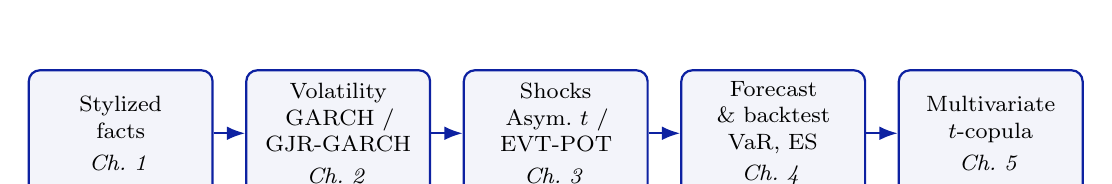
\begin{tikzpicture}[
  node distance=6mm and 4mm,
  box/.style={draw=miAzul, thick, rounded corners, fill=miAzul!5, align=center,
              text width=2.1cm, minimum height=1.6cm, font=\footnotesize},
  arrow/.style={-{Latex}, thick, miAzul}
]
\node[box] (stylized) {Stylized\\facts\\[2pt] \textit{Ch.~1}};
\node[box, right=of stylized] (vol) {Volatility\\GARCH /\\GJR-GARCH\\[2pt] \textit{Ch.~2}};
\node[box, right=of vol] (shock) {Shocks\\Asym.~$t$ /\\EVT-POT\\[2pt] \textit{Ch.~3}};
\node[box, right=of shock] (eval) {Forecast\\\& backtest\\VaR, ES\\[2pt] \textit{Ch.~4}};
\node[box, right=of eval] (copula) {Multivariate\\$t$-copula\\[2pt] \textit{Ch.~5}};

\draw[arrow] (stylized) -- (vol);
\draw[arrow] (vol) -- (shock);
\draw[arrow] (shock) -- (eval);
\draw[arrow] (eval) -- (copula);
\end{tikzpicture}}
\caption*{Modeling pipeline followed throughout the thesis: each stage supplies the inputs required by the next.}
\end{figure}

\section*{Key Results}

Diagnostic checks confirm that the volatility models do their job: after standardizing by the fitted $\sigma_{t+1}^2$, the autocorrelation in squared returns documented in Chapter 1 disappears (Ljung--Box $p$-values of 0.65 and 0.35 for GARCH(1,1) and GJR-GARCH(1,1), respectively), and a likelihood-ratio test confirms that the leverage parameter in GJR-GARCH is statistically significant ($p<0.01$). Goodness-of-fit diagnostics—QQ-plots and empirical-versus-theoretical CDFs—show that the asymmetric $t$-distribution captures the bulk of the standardized-return distribution far better than the normal, while the EVT approach provides a closer fit specifically in the left tail.
\newpage
The risk-management evaluation is where the models' limits become visible. Over the 81-day test window (about 2 breaches expected at the 2.5\% level), the asymmetric-$t$ models produced 5--6 VaR breaches and failed formal coverage tests, whereas the more conservative EVT-based models produced 3--4 breaches and achieved acceptable unconditional coverage. Yet every specification failed the independence test: violations clustered around the sharp volatility spike triggered by the announcement of U.S.\ tariffs in early April 2025, as illustrated below for the GARCH-EVT model, showing that the models—however well calibrated on average—adapt too slowly to abrupt regime changes.

\begin{figure}[H]
    \centering
    \includegraphics[scale=0.17]{4.11.png}
    \caption*{2.5\% VaR, Expected Shortfall, and observed VaR breaches in the Jan.--Apr.\ 2025 test period, GARCH-EVT model (4 breaches observed against 2 expected).}
\end{figure}

\newpage
A subsequent stress test on the 2008 financial crisis confirms the same pattern at a larger scale: every model exceeds its expected breach count, and the gap widens sharply once the crisis intensifies in September--December, as summarized below.

\begin{table}[H]
\centering
\begin{tabular}{lccc}
\toprule
\textbf{Model} & \textbf{Jan--Aug} & \textbf{Sep--Dec} & \textbf{Total} \\
\midrule
GARCH-Asyt & 9 & 7 & 16 \\
GJR-Asyt   & 8 & 5 & 13 \\
GARCH-EVT  & 4 & 5 & 9  \\
GJR-EVT    & 7 & 5 & 12 \\
\midrule
Expected   & 4.17 & 2.10 & 6.28 \\
\bottomrule
\end{tabular}
\caption*{Number of 2.5\% VaR breaches by period and model during the 2008 stress test (167 trading days in Jan.--Aug., 84 in Sep.--Dec.). GARCH-EVT remains the most contained of the four specifications.}
\end{table}

Extending to two assets, the static $t$-copula reproduces the empirical rise in threshold correlations between S\&P 500 and Treasury returns as both series move further into their tails—direct evidence of the nonlinear tail dependence a linear correlation model would miss, as illustrated below—and the resulting portfolio density forecasts pass PIT and Kolmogorov--Smirnov calibration tests. As with the univariate models, however, portfolio VaR breaches remain clustered around the same 2025 volatility shock, and the model's static, symmetric design cannot capture the mild asymmetry observed between the left- and right-tail dependence.

\begin{figure}[H]
    \centering
    \includegraphics[scale=0.43]{5.2.png}
    \caption*{Threshold correlation between GARCH(1,1)-standardized S\&P 500 and 10-year Treasury note returns: correlations rise as both series move deeper into their tails, evidencing heavy-tailed, asymmetric dependence.}
\end{figure}

\section*{Conclusions}

Taken together, the results support a two-part conclusion. On one hand, the modeling pipeline developed here is statistically sound: volatility dynamics are well captured, shock distributions are well fitted in-sample, and density forecasts—both univariate and, via the copula, at the portfolio level—pass calibration diagnostics out-of-sample. On the other hand, every specification considered shares the same practical weakness: none adapts quickly enough to sudden volatility regime shifts, producing clustered VaR violations exactly when accurate risk measurement matters most. The EVT-based tail models mitigate, but do not eliminate, this shortcoming.

These findings should be read against the study's deliberately narrow scope: a bivariate portfolio, a four-month out-of-sample window, parameters fit once on the 2014--2024 sample rather than re-estimated on a rolling basis, and GARCH specifications with fixed lag order and time-invariant tail and copula parameters. Within these bounds, the thesis's central contribution is a complete, reproducible, and empirically grounded "recipe" for return modeling—implemented end to end in \Rlogo\ and openly available at \href{https://github.com/ferpmillan/thesis}{github.com/ferpmillan/thesis}—together with a clear diagnosis of where the standard toolkit falls short. That diagnosis points directly to future work: shock models that let skewness and kurtosis respond dynamically to volatility, and dynamic or asymmetric copula specifications for the multivariate layer.


% Pueden modificar el tamaño del logo cambiando la escala
\newpage
\begin{titlepage}
\begin{center}
\textbf{\LARGE MODELADO DE RENDIMIENTOS FINANCIEROS: VOLATILIDAD CONDICIONAL, COLAS PESADAS Y DEPENDENCIA MULTIVARIADA}\\[2em]
\end{center}
\end{titlepage}
\newpage

\tableofcontents
\mainmatter
\chapter*{Introduction}
\addcontentsline{toc}{chapter}{Introduction}

A PhD student sits in his advisor’s office, scrambling through piles of computer outputs in an attempt to finish a task his advisor assigned. A visiting professor enters, and their ensuing conversation leads to a question so intriguing that it consumes the student’s thoughts overnight. The next morning, he rushes to the lab and begins coding. This is the origin story of the GARCH model, as narrated by \citeA{Bollerslev2023}, who describes the creation of the model as a personal odyssey. At that moment, Bollerslev had little idea of the profound impact his model would have, revitalizing and significantly expanding the literature on financial return modeling. This literature quickly grew, matured, and branched out, generating numerous alternative approaches for nearly every aspect of return modeling. This thesis is, in essence, a consequence of the question posed in 1984 and the extensive literature it subsequently inspired.

The goal of this thesis is to provide a comprehensive overview of financial return modeling. While the thesis acknowledges and discusses alternative methodologies at various modeling stages, it follows a specific path designed to provide the reader with a clear, coherent, and complete narrative. Ultimately, it aims to serve as a concise yet thorough "recipe" for modeling financial returns at the undergraduate level.

Special acknowledgement is due to \citeA{Christoffersen2012}, whose textbook \emph{Elements of Financial Risk Management} served as a guiding reference throughout this work. The aim of presenting the material as a clear, coherent, and reasonably complete narrative was directly inspired by the pedagogical clarity of that text. In the author’s view, Christoffersen’s exposition fills an important gap between the mathematical and statistical foundations typically acquired at the undergraduate level and the more demanding world of quantitative finance. It was through this text that the author first came to appreciate the depth and appeal of financial mathematics.

\hyperref[chap:1]{Chapter 1} outlines the fundamental task of return modeling, highlighting common empirical characteristics that models must capture and replicate. Chapters 2 through 4 then guide the reader through the univariate modeling process. \hyperref[chap:2]{Chapter 2} addresses volatility modeling, \hyperref[chap:3]{Chapter 3} focuses on modeling the distribution of shocks, and \hyperref[chap:4]{Chapter 4} presents methods for rigorously evaluating and testing these models. \hyperref[chap:5]{Chapter 5} extends the framework to a multivariate setting, building coherently on the foundations established in the previous chapters.

All \Rlogo\ code used to generate the analyses and figures is available in the accompanying GitHub repository: \href{https://github.com/ferpmillan/thesis}{github.com/ferpmillan/thesis}.
\newpage
\chapter{Empirical Characteristics of Returns}
\label{chap:1}

The modeling of asset returns has numerous applications, ranging from risk management to asset valuation over time. It is built upon a multi-theoretical foundation in time series analysis and financial theory, drawing insights from a wide range of disciplines. However, modeling asset returns remains an empirical craft, and practical relevance is demanded of these models. This should not come as a surprise, for financial markets are not mere theoretical abstractions; they are living, breathing systems that evolve and play a crucial role in the global economy.

\citeA{Campbell1997} give two main reasons for using returns instead of prices. First, for the average investor, the return of an asset provides a complete and scale-free summary of the investment opportunity. Second, for theoretical and empirical reasons that will become apparent, return series have attractive statistical properties.

We start by defining the daily continuously compounded or log return of an asset from the closing prices of the asset:
\[
R_{t+1}=\ln(S_{t+1})-\ln(S_{t})
\]
where $\ln(*)$ denotes the natural logarithm.

Most financial asset returns exhibit common empirical characteristics—what \citeA{Christoffersen2012} calls the stylized facts of asset returns and what \citeA{Tsay2010} refers to as the empirical properties of returns. \textbf{These empirical characteristics serve as guidelines for what models should capture and replicate}. To illustrate each of these characteristics, we will use daily log returns of the S\&P 500 (Yahoo Finance ticker: \texttt{\textasciicircum{}GSPC}) from January 1, 2014, to December 31, 2024, with closing prices retrieved through the Yahoo Finance API.


Daily log returns exhibit very little autocorrelation. Formally, we can write
\[
\text{Corr}(R_{t+1},R_{t+1-\tau})\approx0 \quad \text{for } \tau = 1,2,3,\ldots \quad. 
\]
This implies that past returns possess little to no predictive power for future returns. Figure~\ref{1.1} displays the autocorrelation function (ACF) of daily S\&P 500 log returns for lags 1 through 100. For lag $\tau$, the ACF is defined as $\rho_\tau = \text{Corr}(R_{t+1},R_{t+1-\tau}).$ For example, at the first lag—that is, the correlation between today’s return and the previous day’s return—the estimated autocorrelation is $\rho_1 = -0.13$.

The dotted lines represent the 95\% confidence interval within which it is statistically reasonable to state that $\rho_\tau = 0$ (under a specific set of assumptions). In the time-series literature, these are commonly referred to as Bartlett’s confidence bands (see, for example, \citeA{Tsay2010}), and are given by $\pm 1.96/\sqrt{T}$. Although there are a few lags for which the estimated autocorrelation falls outside these bands, the overall magnitude of the autocorrelations is small. Given both their low magnitude and the daily frequency of the data, the models developed below assume that the conditional mean of returns is approximately constant, that is, that there is no meaningful linear dependence in returns.
\begin{figure}[H]
    \centering
    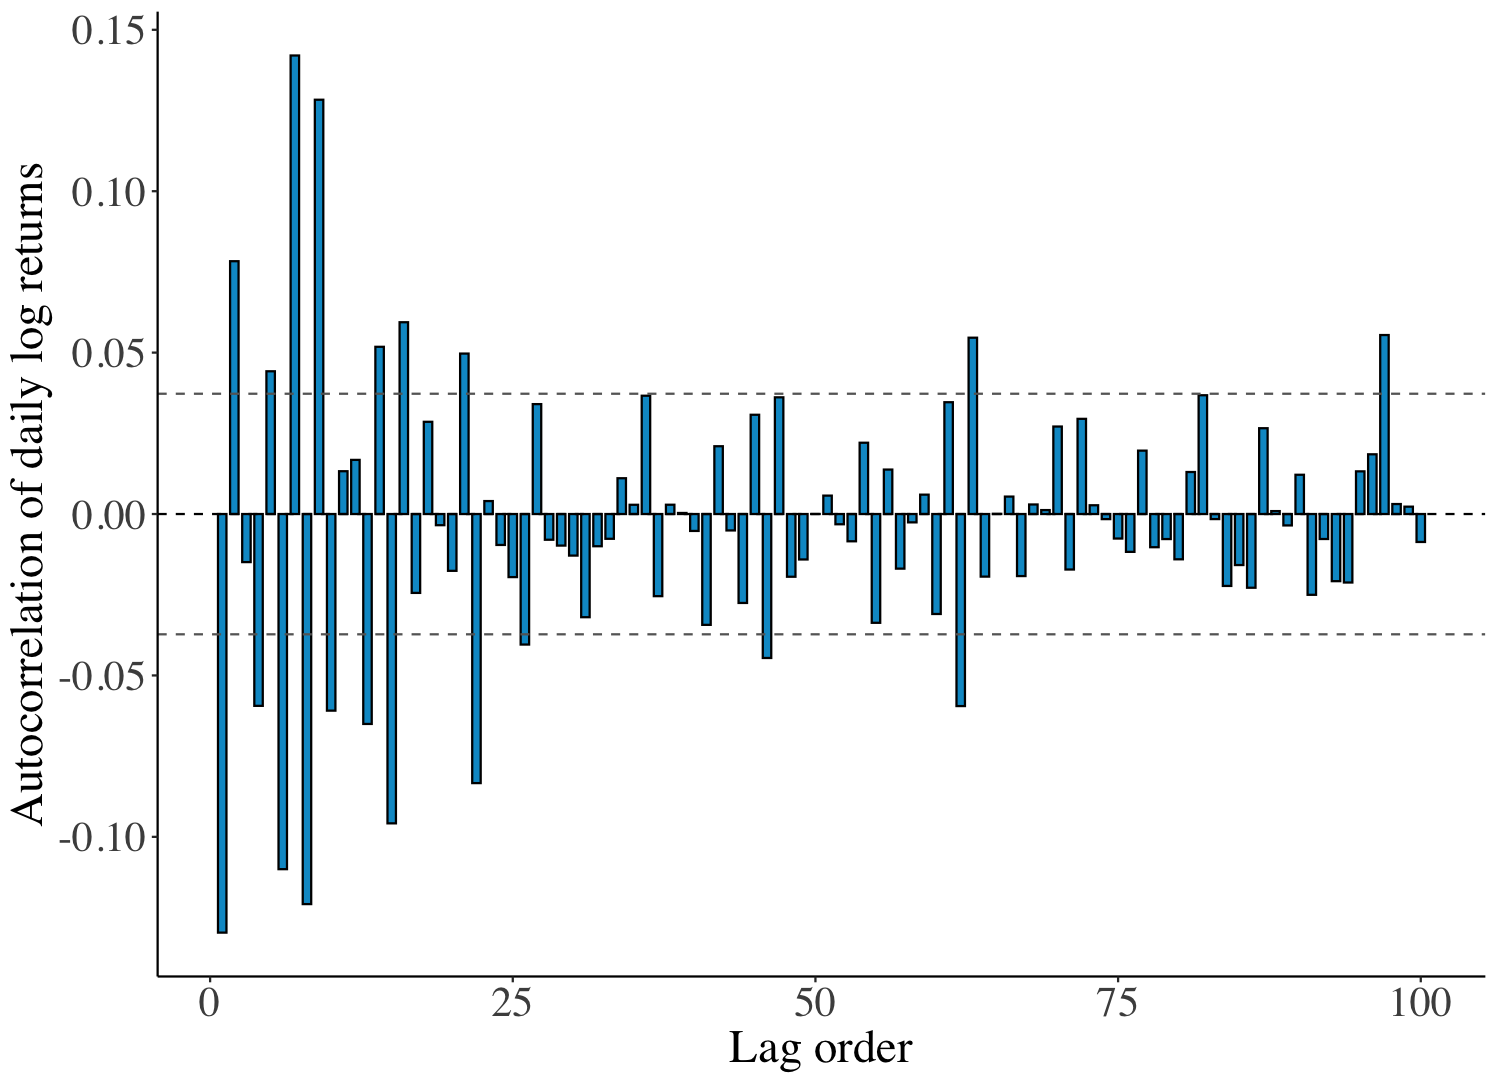
\includegraphics[scale=0.18]{../../plots/1.1.png}
    \caption{Autocorrelation of daily S\&P 500 log returns from January 1, 2014, to December 31, 2024.}
    \label{1.1}
\end{figure}

The unconditional distribution of daily returns departs from normality. Figure~\ref{1.2} shows a histogram of S\&P 500 daily log returns together with a normal density fitted by maximum likelihood. Several features stand out. First, the empirical distribution is more peaked around zero (i.e., leptokurtic). Second, it exhibits heavier tails than the normal, implying a higher probability of extreme outcomes. Third, the distribution is asymmetric: in this sample it displays left-skewness (negative skewness), with a longer left tail than the right. Accurately modeling tail behavior is crucial for risk management, as emphasized by \citeA{Christoffersen2012}.

\begin{figure}[H]
    \centering
    \includegraphics[scale=0.18]{../../plots/1.2.png} % Replace 
    \caption{Histogram of daily S\&P 500 log returns and the normal distribution January 1, 2014 - December 31, 2024. Skewness : -0.8088, Kurtosis : 19.0445   }
    \label{1.2}
\end{figure}

The stock market experiences sharp declines in stock prices and index values, but not equally large upward movements. Consequently, the return distribution exhibits negative skewness.

The standard deviation of returns is considerably larger than the mean at short horizons, such as daily. Statistically, it is reasonable not to reject a zero mean return. Our S\&P 500 data exhibit a daily mean return of 0.0380\% and a daily standard deviation of 1.1211\%.

\pagebreak

Volatility measures, such as squared returns\footnote{Squared returns are commonly used as measures of volatility because, under many return specifications (like the one we discuss below),
$\mathbb{E}[R_t^2 \mid R_{t-1}, R_{t-2}, \ldots] = \sigma_t^2$.
For this reason, the time series of squared returns, $\{R_t^2\}$, becomes relevant for studying volatility dynamics. As noted by \citeA{Christoffersen2012}, squared returns provide an unbiased, though noisy, proxy for conditional variance.}, exhibit positive correlation with their past values, reflecting the tendency of high-volatility events to cluster over time. This effect is most pronounced at short horizons, such as daily returns. Formally, we can write
\[
\text{Corr}(R^2_{t+1},R^2_{t+1-\tau}) > 0 \quad \text{for small } \tau. 
\]
Figure~\ref{1.3} shows the autocorrelation in squared returns for the S\&P 500 data. Models that account for this dependence will be introduced in the next section.

\begin{figure}[H]
    \centering
    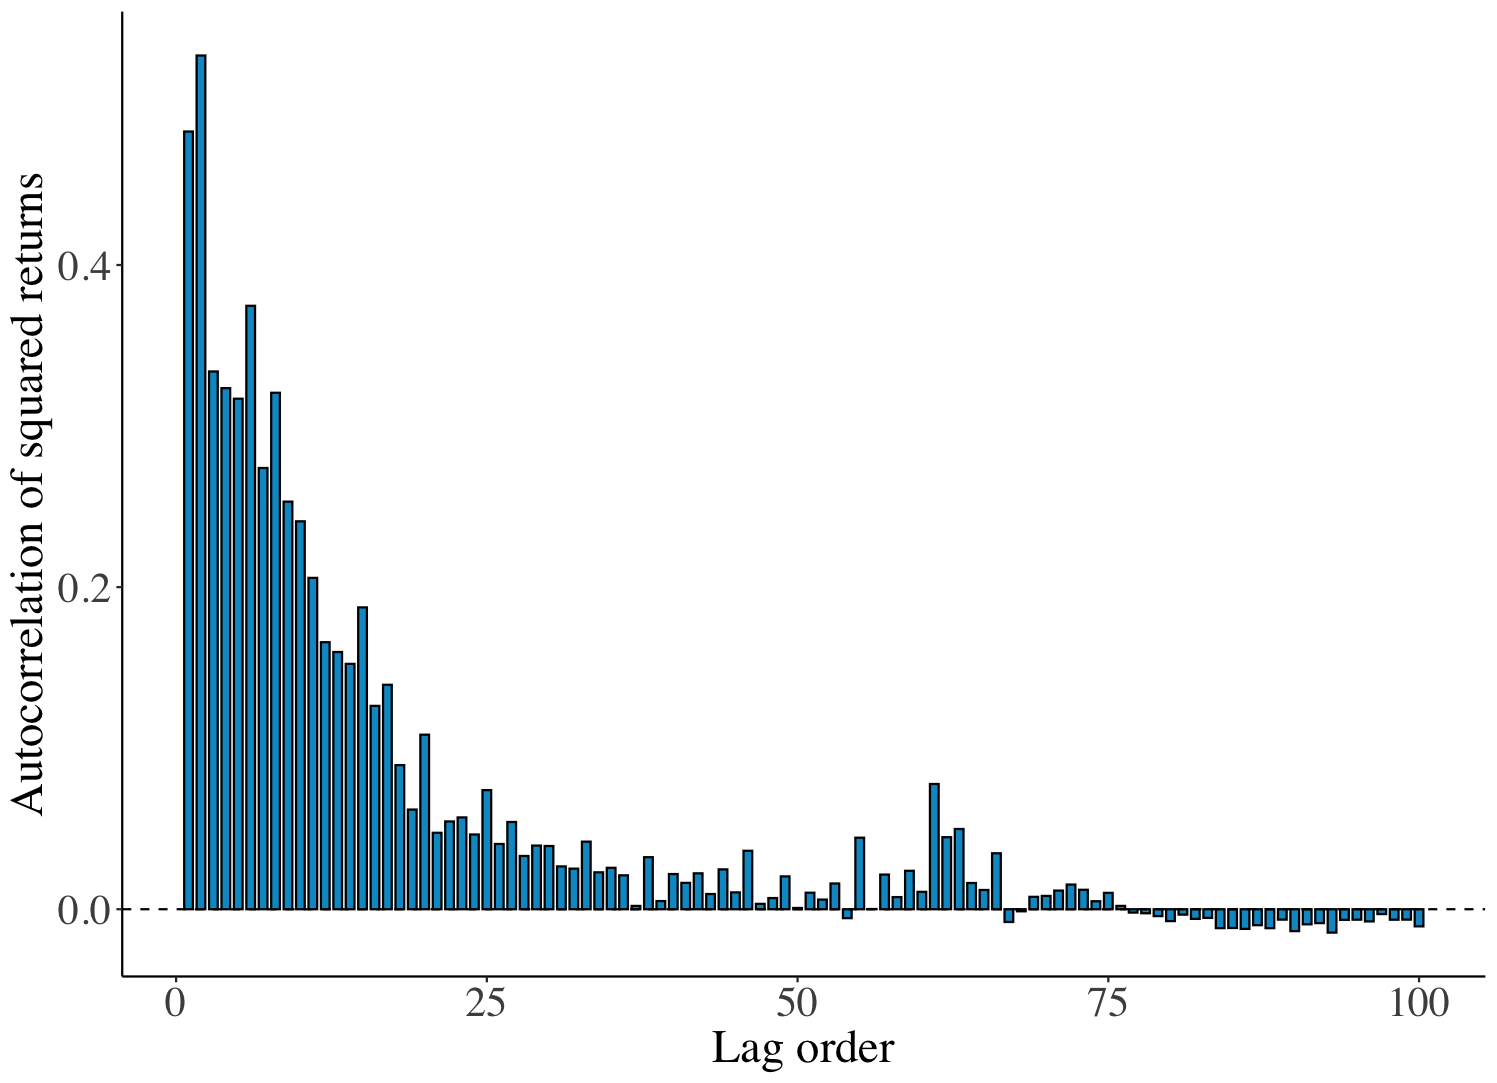
\includegraphics[scale=0.18]{../../plots/1.3.png} % Replace 
    \caption{Autocorrelation of squared daily S\&P 500 log returns from January 1, 2014, to December 31, 2024.}
    \label{1.3}
\end{figure}

For equities and equity indices, asset volatility is negatively correlated with returns. A negative return increases the (conditional) variance more than a positive return of the same magnitude. This phenomenon is known as the leverage effect, arising from the fact that a decrease in a stock’s price increases the firm’s leverage—assuming its debt remains constant—thereby making it riskier.

The correlation among assets appears to vary over time. Notably, it tends to increase in magnitude during highly volatile bear markets and spikes dramatically during market crashes. Figure~\ref{1.4} displays the rolling covariance between S\&P 500 returns and the returns on a 10-year Treasury note index (Bloomberg ticker: \texttt{SPBDU1BT Index}, retrieved via the Bloomberg Terminal), calculated using a 25-day rolling window. A sharp increase in covariance is evident during the early phase of the 2020 pandemic.

\begin{figure}[H]
    \centering
    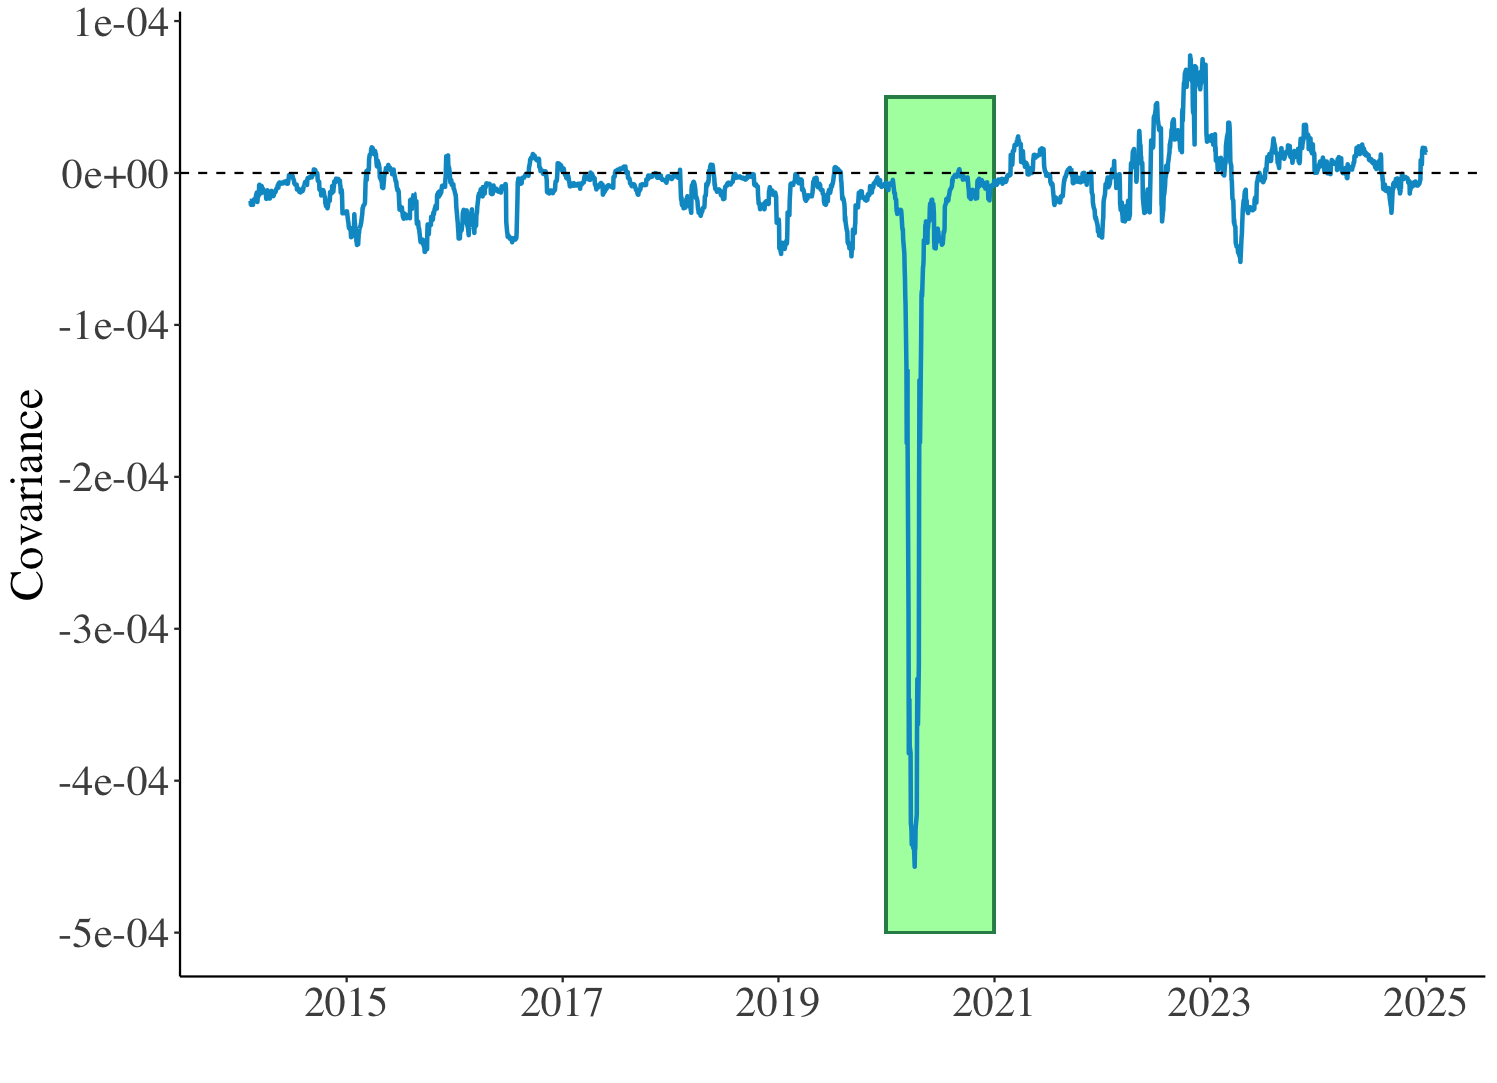
\includegraphics[scale=0.175]{../../plots/1.4.png} % Replace 
    \caption{Rolling covariance between S\&P 500 and 10-year treasury note index.}
    \label{1.4}
\end{figure}

Lastly, even after standardizing returns by time-varying volatility, they continue to exhibit heavier tails than the normal distribution. However, the tails are lighter than those in the unconditional return distribution. This provides evidence of conditional non-normality.

\citeA{Cont2001} provides a detailed discussion of the empirical characteristics of returns presented here, along with additional ones, and examines various statistical challenges that arise in the analysis of financial time series.

Considering the empirical behavior of returns, the model for individual asset returns is
\begin{equation}
R_{t+1}=\mu_{t+1} +\sigma_{t+1}z_{t+1} \quad \text{where } z_{t+1} \sim \text{i.i.d. } D(0,1).
\label{eq:1.1}
\end{equation}
The random variable $z_{t+1}$ represents the innovation term or shock, which we assume to be identically and independently distributed (i.i.d.) with zero mean and unit variance. We assume that the conditional mean of returns, $\mu_{t+1}$, is zero — a reasonable assumption based on the empirical behavior of daily returns discussed earlier. For longer horizons a model for the mean can be necessary\footnote{Readers interested in modeling the conditional mean, $\mu_{t+1}$, are referred to \citeA{Tsay2010} Chapters 2 and 4, and the references therein. \citeA{Tsay2010} provides an exhaustive review of linear and nonlinear models for the conditional mean in financial time series.}, here we focus on modeling daily returns. 

The specification for daily returns is then given by
\begin{equation}
    R_{t+1}=\sigma_{t+1}z_{t+1} \quad \text{where } z_{t+1} \sim \text{i.i.d. } D(0,1).
    \label{eq:1.2}
\end{equation}

\newpage
The univariate and multivariate return models developed in the subsequent chapters are designed to capture and replicate the empirical properties documented in this section. The next section models the conditional volatility, $\sigma_{t+1}$, and the following section models the standardized innovation, $z_{t+1}$.

\newpage
\chapter{Volatility Modeling}
\label{chap:2}

The objective of this chapter is to introduce econometric methods commonly used to model the conditional volatility of asset returns, $\sigma_{t+1}$. These models are collectively referred to as conditional heteroscedastic models.

As noted by \citeA{Tsay2010}, a distinctive feature of stock volatility is that it is not directly observable. Daily volatility cannot be directly inferred from return data because there is only one observation per trading day. However, despite its unobservability, volatility exhibits certain characteristics that are consistently observed in asset returns.

First, as established in the previous chapter, volatility—measured by squared returns—exhibits strong autocorrelation. This implies that if a recent period experienced high variance, the following day is also likely to exhibit high variance, forming what are known as volatility clusters. Figure~\ref{2.1} shows the squared S\&P 500 returns used previously. Observe that volatility is not constant and exhibits distinct clustering patterns.

\begin{figure}[H]
    \centering
    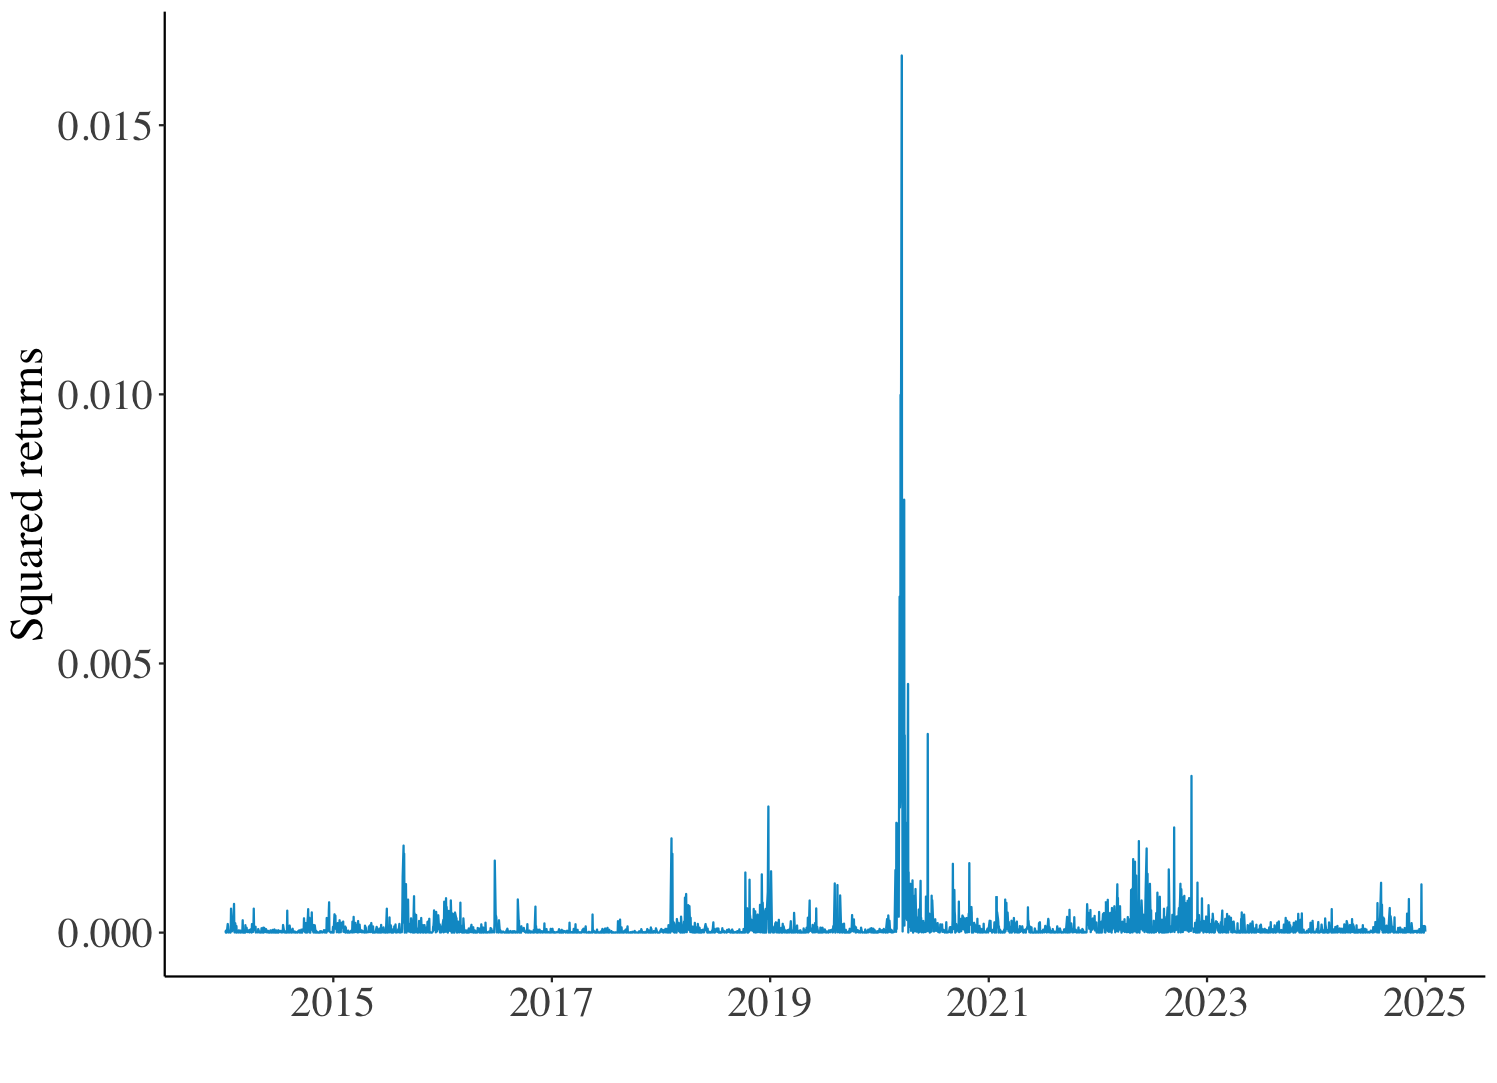
\includegraphics[scale=0.18]{../../plots/2.1.png} % Replace 
    \caption{Squared S\&P 500 returns, 2014-2024.}
    \label{2.1}
\end{figure}

Additionally, volatility evolves continuously over time, does not diverge to infinity, and, as previously discussed, appears to respond asymmetrically to large price increases and decreases.

The literature on volatility models is extensive. Early models were developed to capture the dynamic dependency observed in variance, and subsequent models were introduced to address the limitations of their predecessors, particularly their inability to fully capture the characteristics discussed earlier. Over time, a wide range of volatility models has emerged, each catering to different modeling needs.
\newpage
Before introducing specific volatility models, the squared return series, $R^2_{t+1}$ can be used to check for conditional heteroscedasticity. The Ljung–Box statistic \cite{McLeod1983} is commonly employed for this purpose, testing the null hypothesis that the first $m$ lags of the autocorrelation function (ACF) of the squared series are zero. Applying this test to the squared S\&P 500 returns with $m=\ln(T)\approx7$ \footnote{Setting $m = \ln(T)$
has been found to work well in simulation studies, as noted by \citeA{Christoffersen2012}.}, the p-value is close to zero. 


Two volatility models will be considered: the GARCH(1,1) model of \citeA{Bollerslev1986} and the GJR-GARCH model of \citeA{Glosten1993}. The GARCH(1,1) model is included because, despite its simplicity, it remains the go-to volatility model for many applied researchers—not only in finance but also in broader fields. Remarkably, GARCH(1,1) has proven difficult to convincingly outperform in out-of-sample forecasting, maintaining its status as the dominant benchmark. \citeA{Bollerslev2023} provides a historical overview of the GARCH model’s origins and discusses its widespread adoption, emphasizing the enduring supremacy of GARCH(1,1). The GJR-GARCH model is considered because it is the simplest extension of GARCH designed to capture the leverage effect, making it a natural choice among asymmetric volatility models.

As previously mentioned, there is a volatility model for every need. Various modifications of the GARCH model have been developed to address specific features of financial data. Some, such as EGARCH and GJR-GARCH, are designed to capture the leverage effect, while others, like IGARCH, aim to better describe long-run dynamic dependencies. Additional extensions include models that incorporate explanatory variables or integrate financial theory, such as the GARCH-M model. Many other variations exist, each tailored to different modeling objectives. Another class of volatility models not considered here is stochastic volatility models. Compared to GARCH models, they offer greater flexibility but are more challenging to estimate. \citeA{Bollerslev2010} provides a comprehensive guide to GARCH extensions, and \citeA{Tsay2010} and \citeA{Christoffersen2012} each dedicate a chapter in their books to volatility modeling, offering thorough reviews of the literature.

The fundamental idea in volatility modeling is that the return series $R_{t+1}$ is either serially uncorrelated or exhibits only minor lower-order serial correlations, yet it remains dependent through its conditional variance. As noted by \citeA{Tsay2010}, it is the time evolution of $\sigma^2_{t+1}$ that distinguishes one volatility model from another.

Recall that the return series follows Equation~\eqref{eq:1.2}. In the GARCH(1,1) model, the conditional variance evolves as
\begin{equation}
    \sigma^2_{t+1} = \omega + \alpha R^2_{t} + \beta\sigma^2_{t}
    \label{eq:2.1}
\end{equation}
with $ \omega > 0,\ \alpha \geq 0,\ \beta \geq 0,\ \alpha + \beta < 1$. These restrictions ensure that the conditional variance is positive and that the process has a finite long-run variance. For the GJR-GARCH(1,1) model, the conditional variance is:
\begin{equation}
    \sigma^2_{t+1} = \omega + \alpha R^2_{t} + \alpha \theta I_{t} R^2_{t} + \beta\sigma^2_{t}
    \label{eq:2.2}
\end{equation}
where $I_t=\mathbf{1}\{R_t<0\}$. Here, $\omega>0$, $\alpha\geq0$, $\theta\geq0$, and $\beta\geq0$ guarantee positivity of the conditional variance, and $\alpha\left(1+\frac{\theta}{2}\right)+\beta<1$ ensures the existence of a finite long-run variance under symmetric innovations. A positive $\theta$ captures the leverage effect.
\newpage

To estimate the parameters of each model, we must assume a distribution for $z_{t+1}$ in Equation~\eqref{eq:1.2}. However, we can set aside this assumption for now, as the modeling of $z_{t+1}$ will be discussed in the next section. For the time being, we will use quasi-maximum likelihood estimation (QMLE), which refers to the application of normal maximum likelihood estimation even when the normality assumption does not necessarily hold.\footnote{A key result in econometrics states that even if the conditional distribution is not normal, MLE provides consistent estimates of the mean and variance parameters as the sample size approaches infinity, provided that the mean and variance functions are correctly specified \cite{Christoffersen2012}. \citeA{francq2010garch} provide a comprehensive treatment of quasi-maximum likelihood estimation (QMLE) for GARCH models, including key results such as consistency, asymptotic normality, and their proofs.}

Under the temporary assumption that \(z_{t+1}\sim \mathcal{N}(0,1)\), the conditional distribution of returns implied by Equation~\eqref{eq:1.2} is
\[
R_{t+1}\mid \mathcal{F}_t \sim \mathcal{N}(0,\sigma^2_{t+1}),
\]
where \(\mathcal{F}_t\) denotes the information set available at time \(t\). The corresponding conditional density is therefore
\[
f(R_{t+1}\mid \mathcal{F}_t;\vartheta)
=
\frac{1}{\sqrt{2\pi\sigma^2_{t+1}}}
\exp\left(
-\frac{R_{t+1}^2}{2\sigma^2_{t+1}}
\right),
\]
where \(\vartheta\) collects the volatility parameters. For the GARCH(1,1) model,
\[
\vartheta=(\omega,\alpha,\beta),
\]
while for the GJR-GARCH(1,1) model,
\[
\vartheta=(\omega,\alpha,\beta,\theta).
\]

Given a sample \(\{R_t\}_{t=1}^T\), the conditional log-likelihood under normality is
\[
\ell(\vartheta)
=
\sum_{t=1}^T \log f(R_t\mid \mathcal{F}_{t-1};\vartheta)
=
-\frac{1}{2}\sum_{t=1}^T
\left[
\log(2\pi)+\log(\sigma_t^2)+\frac{R_t^2}{\sigma_t^2}
\right].
\]
Since \(\log(2\pi)\) is constant, maximizing the likelihood is equivalent to minimizing
\[
\sum_{t=1}^T
\left[
\log(\sigma_t^2)+\frac{R_t^2}{\sigma_t^2}
\right].
\]

The QMLE estimator is then obtained as
\[
\hat{\vartheta}
=
\arg\max_{\vartheta\in\Theta}\,\ell(\vartheta),
\]
subject to the parameter restrictions imposed previously to ensure positivity of the conditional variance and existence of a finite long-run variance. In practice, this optimization is carried out numerically, since the likelihood has no closed-form maximizer\footnote{The likelihood has no closed-form maximizer because the parameters enter the objective function through the recursive variance equation, making the likelihood a nonlinear function of the full conditional variance path.}. Each trial value of \(\vartheta\) generates a full sequence \(\{\sigma_t^2\}_{t=1}^T\) through the corresponding volatility recursion, and the value of the log-likelihood is then evaluated at that sequence.

To start the recursion, an initial variance must be specified. A common choice is to use the sample variance of returns or the unconditional variance implied by the model whenever it exists. Once the initial value is fixed, the recursion produces the entire path of conditional variances needed to evaluate the likelihood.

Figures \ref{2.2} and \ref{2.3} display the squared S\&P 500 returns from Figure \ref{2.1}, now with the estimated variance from the GARCH(1,1) and GJR-GARCH(1,1) models superimposed, respectively. The parameters were estimated using the full sample (2014–2024), and the figures show the model’s performance over this same estimation period. Out-of-sample forecasting and its evaluation will be discussed in \hyperref[chap:4]{Chapter 4}.

Using QMLE, the optimal parameter estimates yield the following variance dynamics for the GARCH(1,1):
\begin{equation}
\begin{aligned}
    \sigma^2_{t+1} &= \omega + \alpha R^2_t + \beta \sigma^2_t \\
                   &=  0.0000039 + 0.171R^2_{t} +  0.794 \sigma^2_{t}.
\end{aligned}
\label{eq:2.3}
\end{equation}

For the GJR-GARCH(1,1): 
\begin{equation}
\begin{aligned}
    \sigma^2_{t+1} &= \omega + \alpha R^2_{t} + \alpha \theta I_{t} R^2_{t}+ \beta\sigma^2_{t} \\
                   &= 0.0000040 + 0.054R^2_{t} + 0.248 I_{t} R^2_{t}+ 0.795\sigma^2_{t}.
\end{aligned}
\label{eq:2.4}
\end{equation}

\begin{figure}[H]
    \centering
    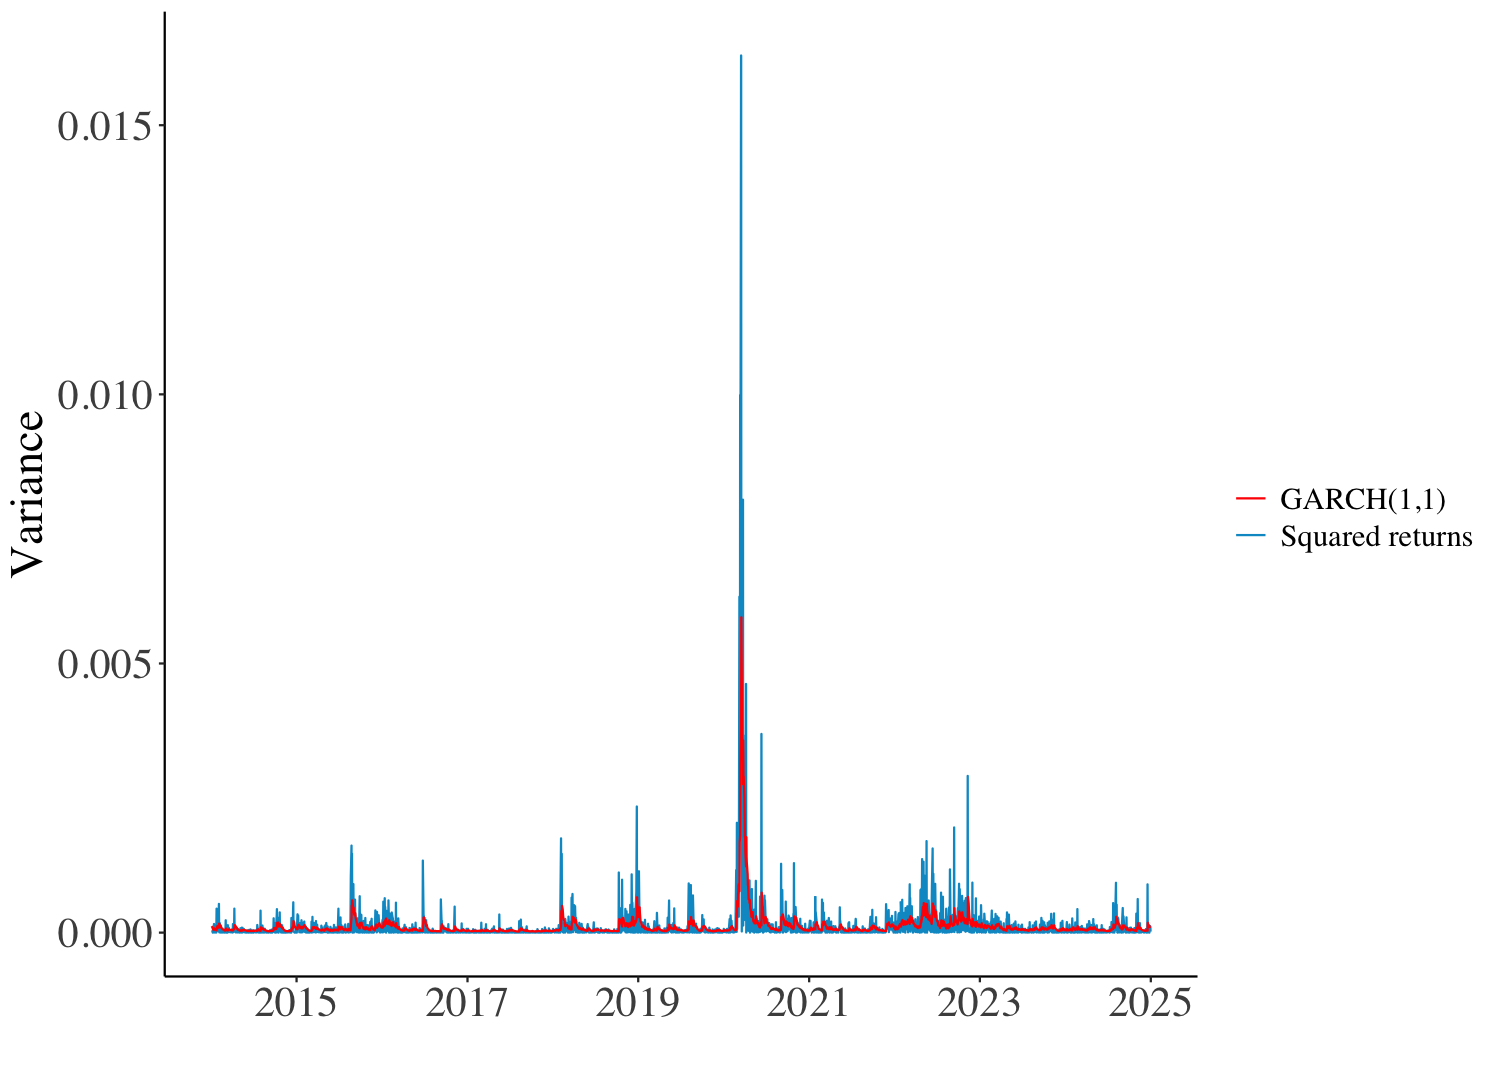
\includegraphics[scale=0.16]{../../plots/2.2.png} % Replace 
    \caption{Squared S\&P 500 returns with GARCH(1,1) variance parameters estimated using
QMLE.}
    \label{2.2}
\end{figure}


\begin{figure}[H]
    \centering
    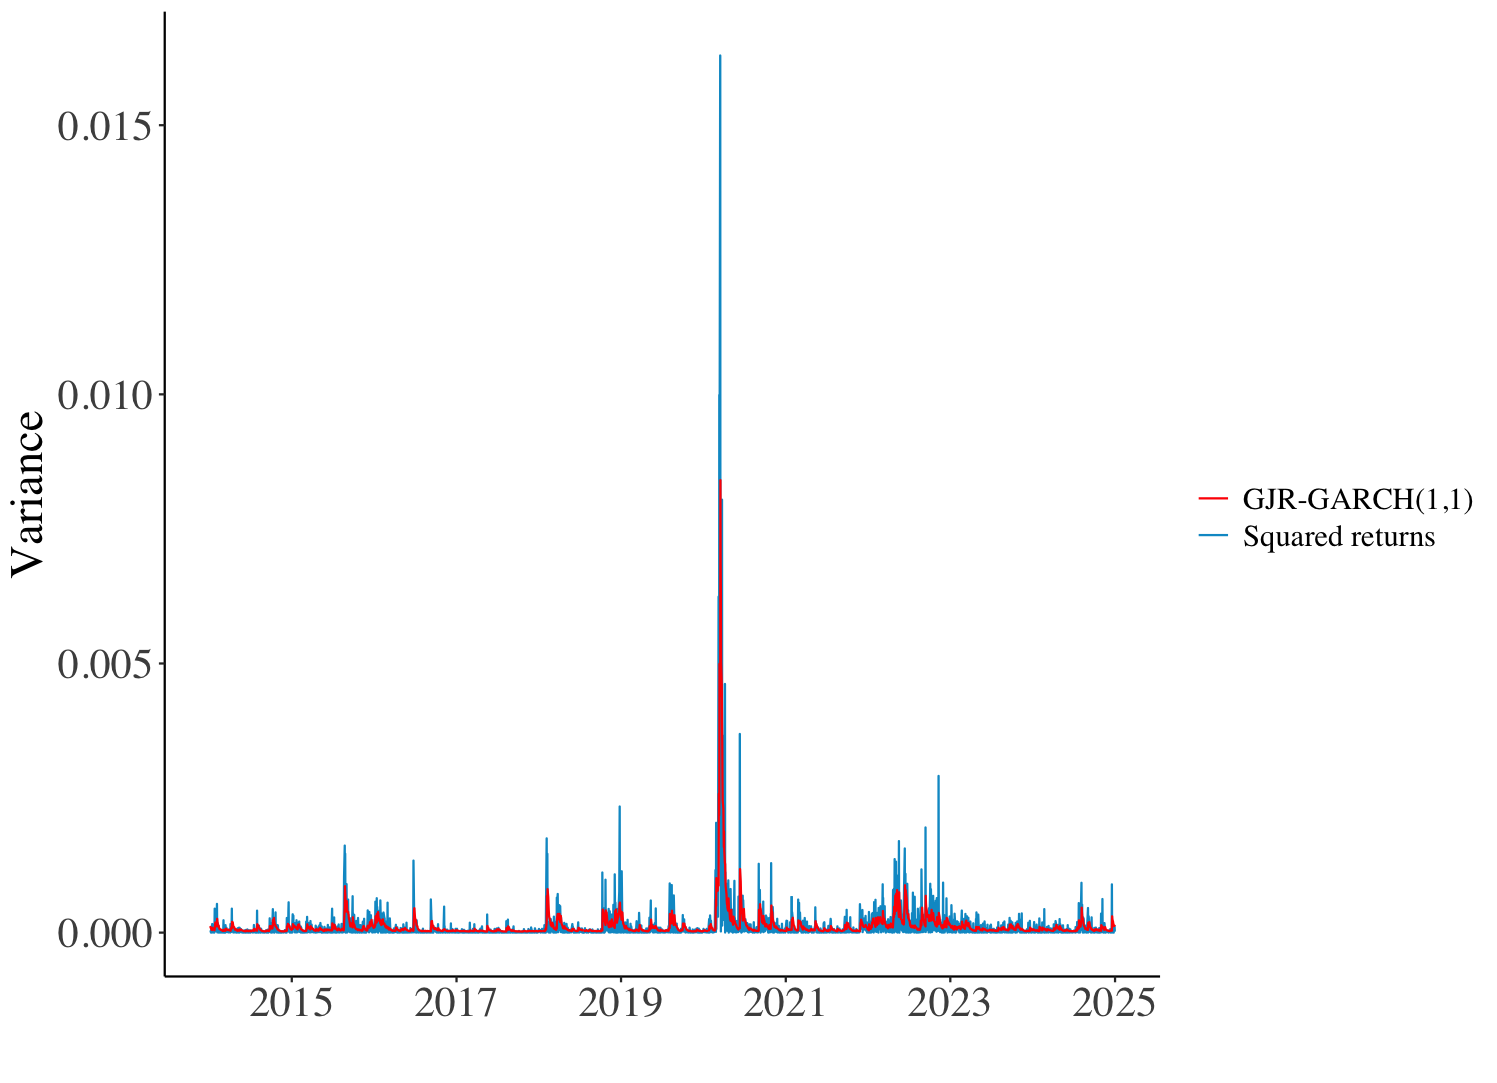
\includegraphics[scale=0.165]{../../plots/2.3.png} % Replace 
    \caption{Squared S\&P 500 returns with GJR-GARCH(1,1) variance parameters estimated using
QMLE.}
    \label{2.3}
\end{figure}

GARCH models possess several desirable theoretical properties that have been studied extensively, including the existence of a long-run variance and the ability to produce longer-horizon forecasts—features that may be relevant for risk management applications. In this chapter, we focus on daily returns and daily volatility forecasts.

Observe that $\alpha+\beta \approx 1$ in the fitted GARCH(1,1), and $\alpha+\beta+\alpha\theta\,\mathbb{E}[I_t]\approx1$ in the GJR–GARCH(1,1); under symmetric innovations $\mathbb{E}[I_t]=\tfrac{1}{2}$, giving $\alpha+\beta+\tfrac{1}{2}\alpha\theta \approx 1$. This near-unit persistence is common in financial return series \cite{Christoffersen2012}. When the persistence parameter equals one, i.e.\ $\alpha+\beta=1$ for GARCH(1,1) and $\alpha+\beta+\alpha\theta\,\mathbb{E}[I_t]=1$ for GJR–GARCH(1,1), the variance dynamics have a unit root (the IGARCH model case): the unconditional variance is not finite and multi-step variance forecasts do not mean-revert to a constant long-run level. As noted by \citeA{Tsay2010}, $\{\sigma_t^2\}$ is a martingale\footnote{A stochastic process \(\{X_t\}\) is a martingale with respect to an information set \(\{\mathcal{F}_t\}\) if its conditional expectation satisfies \(\mathbb{E}[X_{t+1}\mid\mathcal{F}_t]=X_t\). Intuitively, given current information, the best forecast of tomorrow’s value is today’s value.} in this setting, and the sources of volatility persistence warrant careful investigation.

Another important theoretical feature of GARCH models is their ability to generate return distributions with heavier tails than the normal distribution, even when normality is assumed for $z_{t+1}$. This means the volatility model itself contributes to capturing the excess kurtosis commonly observed in financial returns. \citeA{Bai2003} derive the kurtosis of GARCH models and show that, provided the kurtosis exists, the distribution of returns under a GARCH process can indeed exhibit heavier tails than the normal distribution.

Having analyzed return volatility, the next step is to properly model $z_{t+1}$, the standardized return or shock—keeping in mind the ultimate goal: to capture and replicate the empirical behavior of returns. The evaluation of the volatility models will be deferred to \hyperref[chap:4]{Chapter 4}, once the complete model for the return $R_{t+1}$ has been specified.
\newpage
\newpage
\chapter{Shock Modeling}
\label{chap:3}

The focus now shifts to modeling the innovation $z_{t+1}$ in Equation~\eqref{eq:1.2}. The heterscedastic models introduced in the previous chapter help capture the excess kurtosis observed in returns. However, the distribution of the standardized return, $z_{t+1} = \frac{R_{t+1}}{\sigma_{t+1}}$, remains a challenge, as the assumption of normality is not necessarily appropriate.

Figures \ref{3.1} and \ref{3.2} display histograms of returns standardized using the conditional volatility from the GARCH(1,1) and GJR-GARCH(1,1) models, respectively. The empirical distribution of standardized returns continues to deviate from the standard normal distribution, exhibiting heavy tails, a degree of asymmetry, and a more pronounced peak around zero.\footnote{A Kolmogorov–Smirnov test performed on both sets of standardized returns strongly rejects the null hypothesis of standard normality, with p-values below 0.005\%. For an extensive survey of the approaches used in financial econometrics to assess and model non-normality in returns, see \citeA{Pagan1996}.}

\begin{figure}[H]
    \centering
    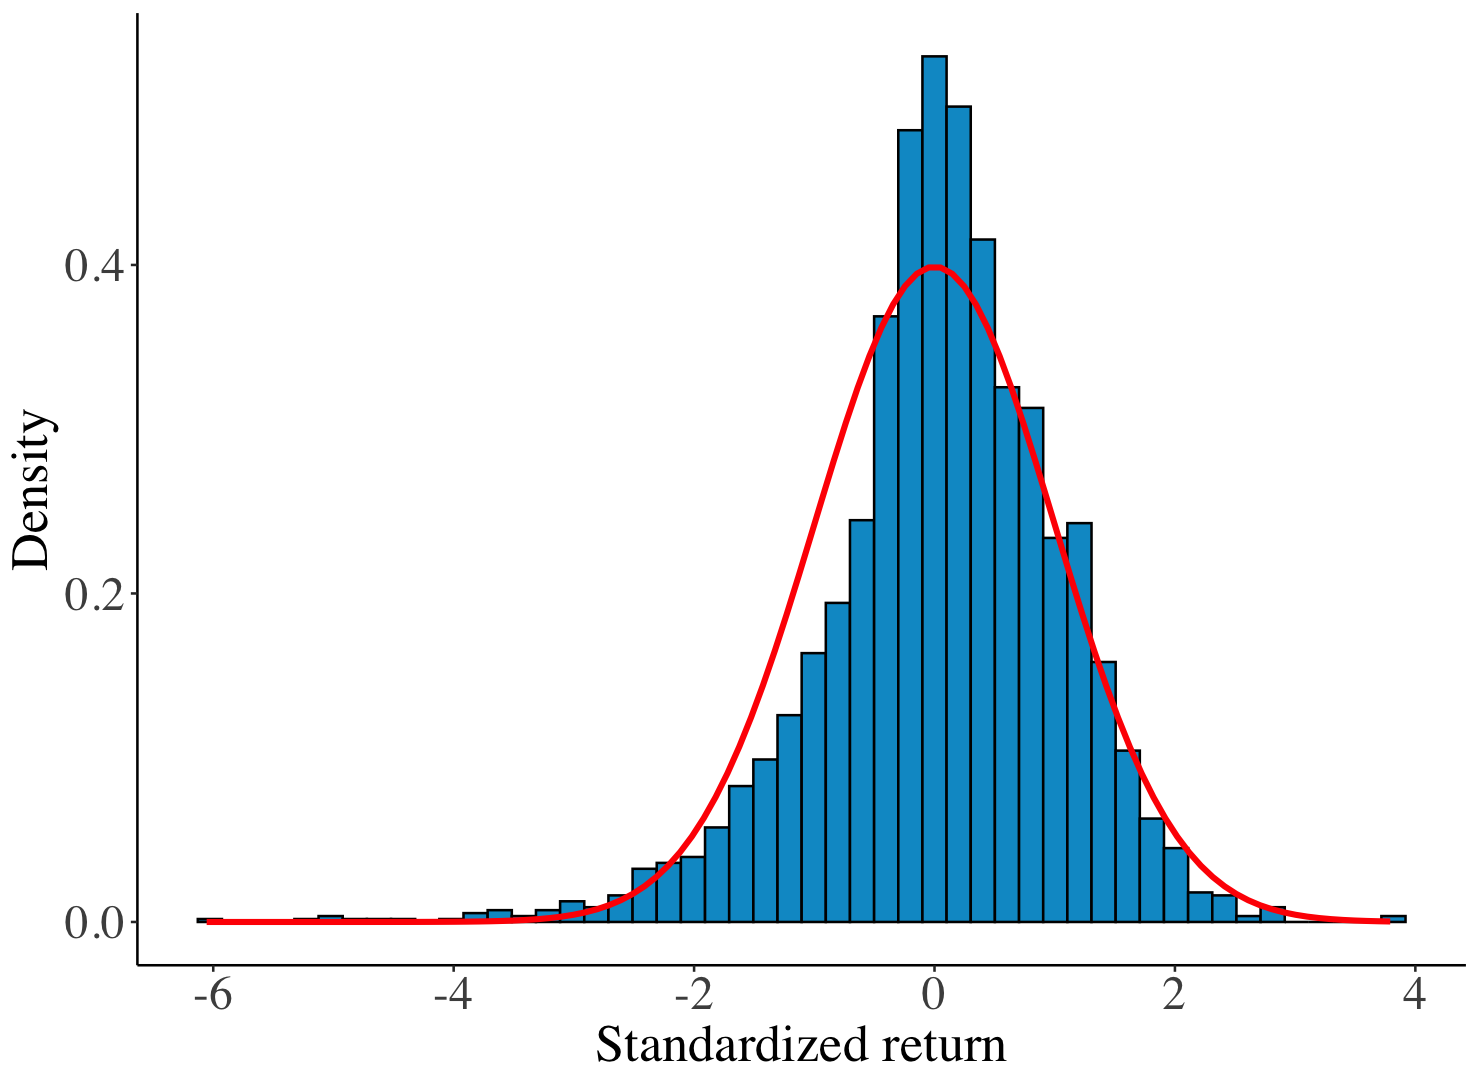
\includegraphics[scale=0.18]{../../plots/3.1.png} % Replace 
    \caption{Histogram of standardized returns, GARCH(1,1).}
    \label{3.1}
\end{figure}

\begin{figure}[H]
    \centering
    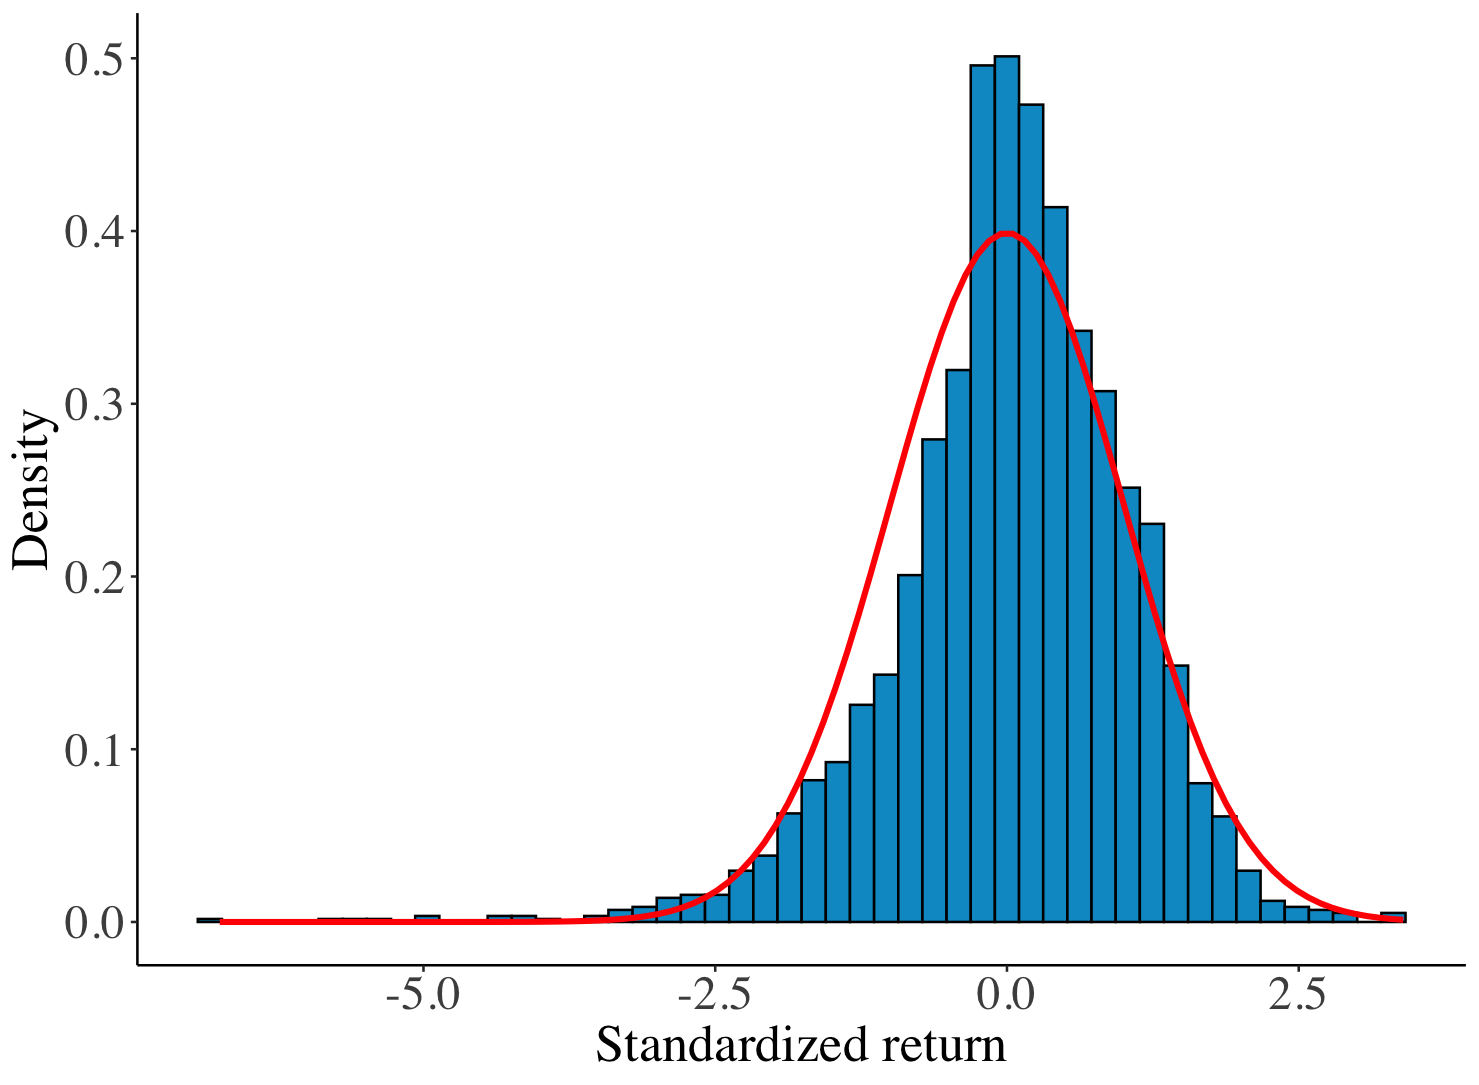
\includegraphics[scale=0.18]{../../plots/3.2.png} % Replace 
    \caption{Histogram of standardized returns, GJR-GARCH(1,1).}
    \label{3.2}
\end{figure}

\newpage

To further illustrate the limitations of the normality assumption, consider the normal QQ plots of both sets of residuals shown in Figures \ref{3.3} and \ref{3.4}. A particularly important weakness is the inability of the normal distribution to capture the left tail of the empirical distribution, which is considerably heavier. This has critical implications for risk management, as underestimating the probability of extreme negative returns leads to an underestimation of market risk.

\begin{figure}[H]
    \centering
    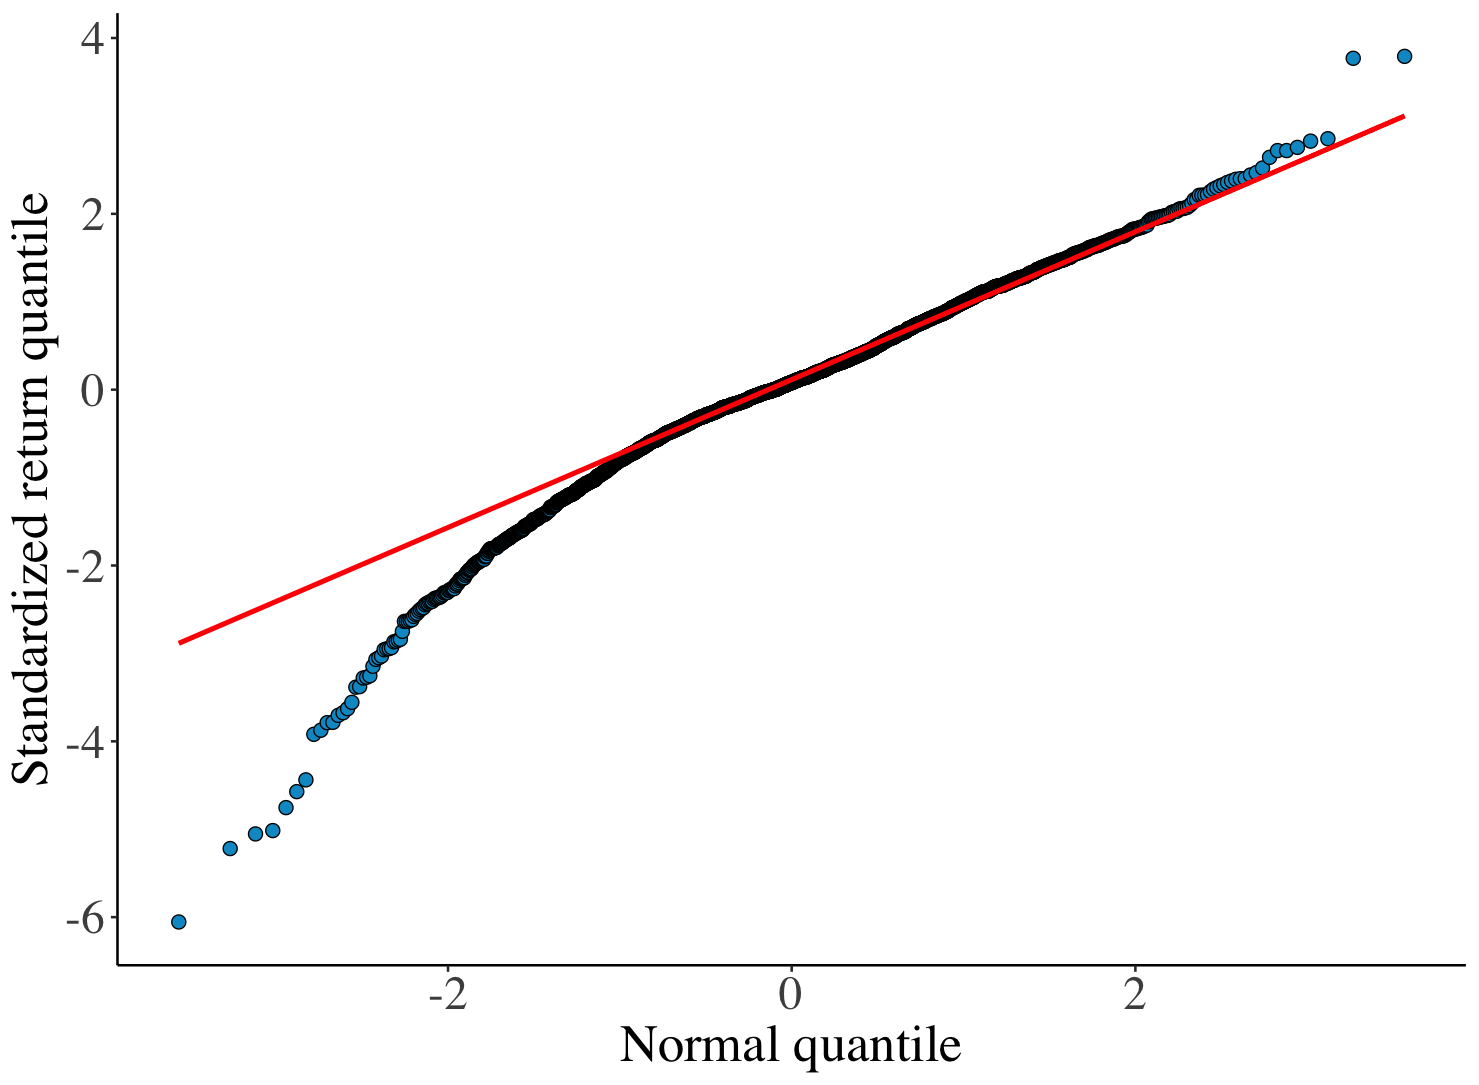
\includegraphics[scale=0.18]{../../plots/3.3.png} % Replace 
    \caption{Normal QQ plot of daily standardized S\&P 500 returns, GARCH(1,1).}
    \label{3.3}
\end{figure}

\begin{figure}[H]
    \centering
    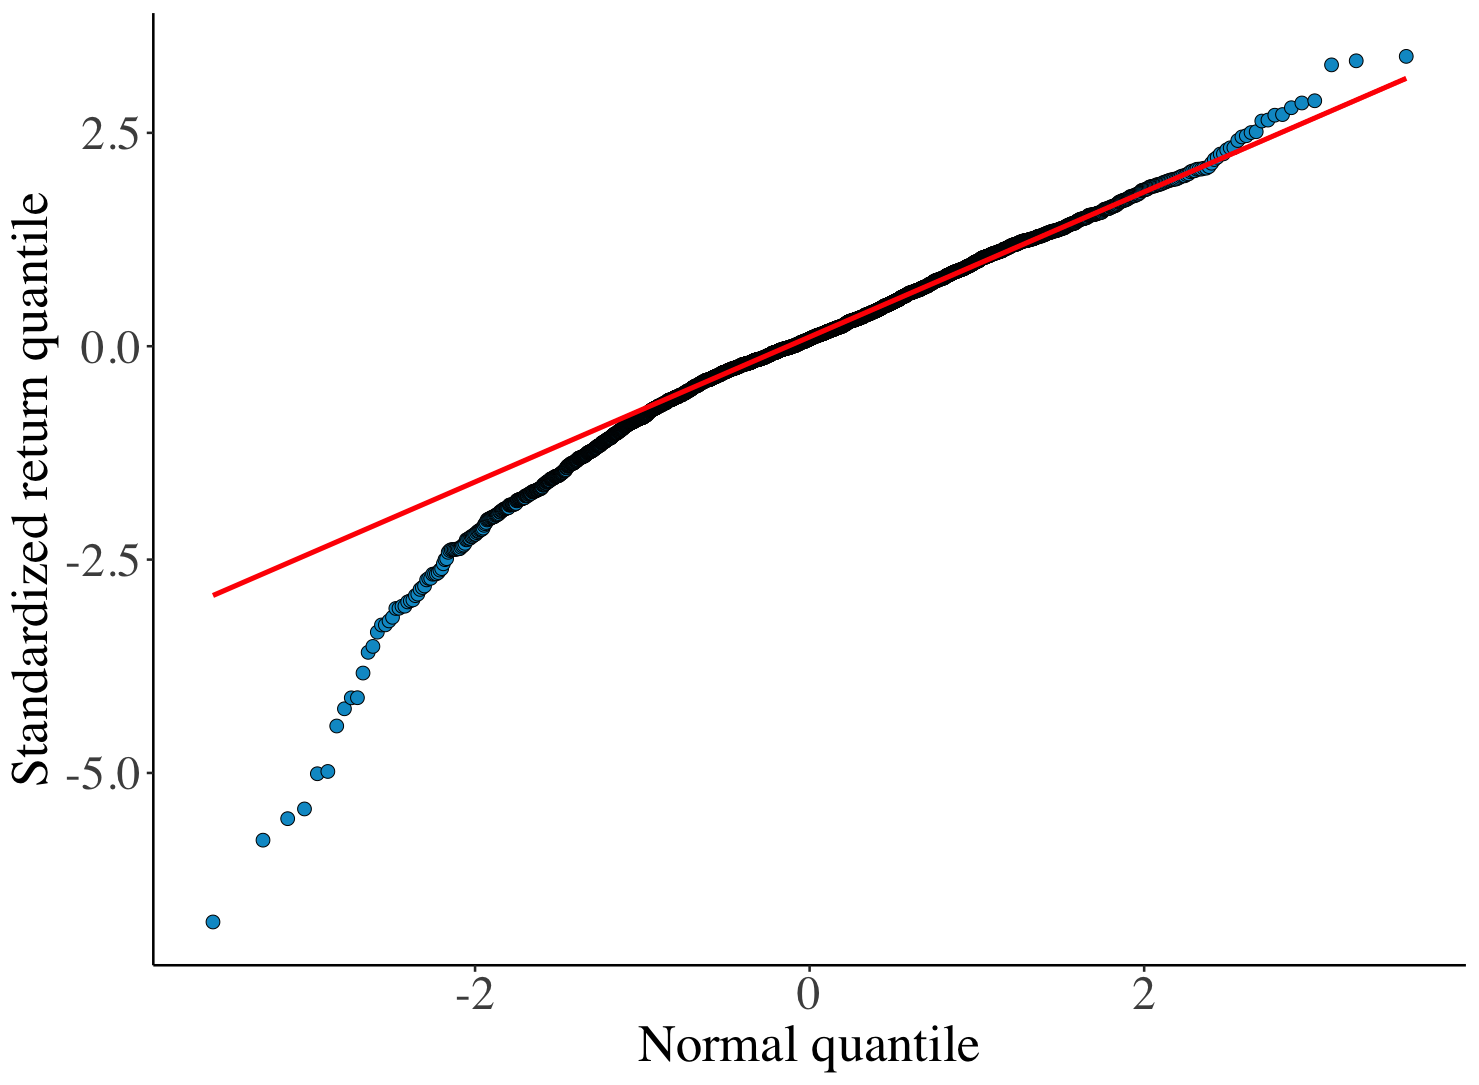
\includegraphics[scale=0.18]{../../plots/3.4.png} % Replace 
    \caption{Normal QQ plot of daily standardized S\&P 500 returns, GJR-GARCH(1,1).}
    \label{3.4}
\end{figure}
The objective is to identify a distribution that adequately fits the standardized returns, ensuring the model specified in Equation~\eqref{eq:1.2}, with the assumption $z_{t+1} \sim \text{i.i.d. } D(0,1)$, is appropriate. To overcome the limitations of the standard normal distribution, two alternative approaches are considered: an asymmetric extension of the standardized Student’s $t$-distribution, and extreme value theory.

\newpage
As \citeA{Cont2001} states, fitting various functional forms to the distribution of stock returns and stock price changes has become a popular pastime. Numerous parametric models have been proposed in the literature, starting with the normal distribution and extending to stable distributions, Student’s $t$-distribution\footnote{\citeA{Bollerslev1987} introduced an extension to the GARCH and ARCH models by allowing for conditionally $t$-distributed errors.}, and hyperbolic distributions\footnote{Stable distributions are a family of distributions closed under addition. Hyperbolic distributions are a flexible class of heavy-tailed distributions whose log-density has the shape of a hyperbola—hence the name. Because the logarithm of the density decays approximately linearly rather than quadratically in the tails, as in the normal case, hyperbolic distributions assign more probability to extreme outcomes and therefore have heavier tails than the normal distribution.}, among others. Given the empirical features discussed in \hyperref[chap:1]{Chapter 1}, a parametric distribution capable of capturing all these properties should have at least four parameters: a location parameter, a scale (volatility) parameter, a parameter governing tail behavior, and an asymmetry parameter allowing distinct behaviors for the left and right tails. The first of the approaches considered here—the asymmetric standardized $t$-distribution—meets these criteria.

The asymmetric standardized $t$-distribution, alternatively derived by \citeA{Fernandez1998}, provides a skewed extension of the Student’s $t$-distribution, enabling the modeling of both kurtosis and skewness observed in standardized returns. The probability density function (PDF) is defined as follows: 

\begin{equation}
f_{\text{asyt}}(z; d_1, d_2) =
\begin{cases}
B \thinspace C \left[ 1 + \dfrac{(Bz + A)^2}{(1 - d_2)^2 (d_1 - 2)} \right]^{-\frac{1 + d_1}{2}}, & \text{if } z < -A/B \\
B \thinspace C \left[ 1 + \dfrac{(Bz + A)^2}{(1 + d_2)^2 (d_1 - 2)} \right]^{-\frac{1 + d_1}{2}}, & \text{if } z \geq -A/B
\end{cases}
\label{eq:3.1}
\end{equation}
\noindent\text{where}
\[
A = 4\thinspace d_2\thinspace C  \thinspace  \dfrac{d_1 - 2}{d_1 - 1}, \quad
B = \sqrt{1 + 3d_2^2 - A^2}, \quad
C = \dfrac{\Gamma\left( \frac{d_1 + 1}{2} \right)}{\Gamma\left( \frac{d_1}{2} \right) \sqrt{\pi (d_1 - 2)}},
\]
and where $d_{1} > 2$, and $-1 < d_{2} < 1$. \citeA{Hansen1994} demonstrates that this is a proper density function and applies it to the U.S. Dollar/Swiss Franc exchange rate. A random variable following this distribution has zero mean, unit variance, and skewness and kurtosis that are nonlinear functions of $d_1$ and $d_2$ \cite{Christoffersen2012}. 

Thus, the first complete univariate model for daily returns is defined as:
\begin{equation}
    R_{t+1}=\sigma_{t+1}z_{t+1} \quad \text{where } z_{t+1} \sim \text{i.i.d. asyt}(d_1,d_2),
    \label{eq:3.2}
\end{equation}
with conditional variance $\sigma^2_{t+1}$ given by either the GARCH(1,1):
\begin{equation}
   \sigma^2_{t+1} = \omega + \alpha R^2_t + \beta \sigma^2_t,
    \label{eq:3.3}
\end{equation}
or the GJR-GARCH(1,1):
\begin{equation}
  \sigma^2_{t+1} = \omega + \alpha R^2_t + \alpha \theta I_t R^2_t + \beta \sigma^2_t.
    \label{eq:3.4}
\end{equation}

\citeA{Christoffersen2012} discusses various methods for estimating the model given by Equation~\eqref{eq:3.2}. In the approach followed here, the volatility parameters are first estimated using quasi-maximum likelihood estimation, and then the parameters $d_1$ and $d_2$ are estimated by maximizing the likelihood under the asymmetric Student’s $t$-distribution.

Once the parameters of the model have been estimated (the values of $d_1$ and $d_2$ for both fits are reported in Table~\ref{tab:3.1}), the goodness-of-fit can be evaluated visually and compared with the results obtained under the normality assumption. Figures~\ref{3.5} and~\ref{3.6} display histograms of standardized returns from the GARCH(1,1) and GJR-GARCH(1,1) models, respectively, along with their fitted asymmetric Student’s $t$-distributions. These figures show that the asymmetric $t$-distribution better captures both the pronounced central peak and the skewness present in standardized returns. Additionally, the tails of the fitted distribution are heavier than those of the normal distribution, offering a closer replication of the empirical characteristics.

\begin{figure}[H]
    \centering
    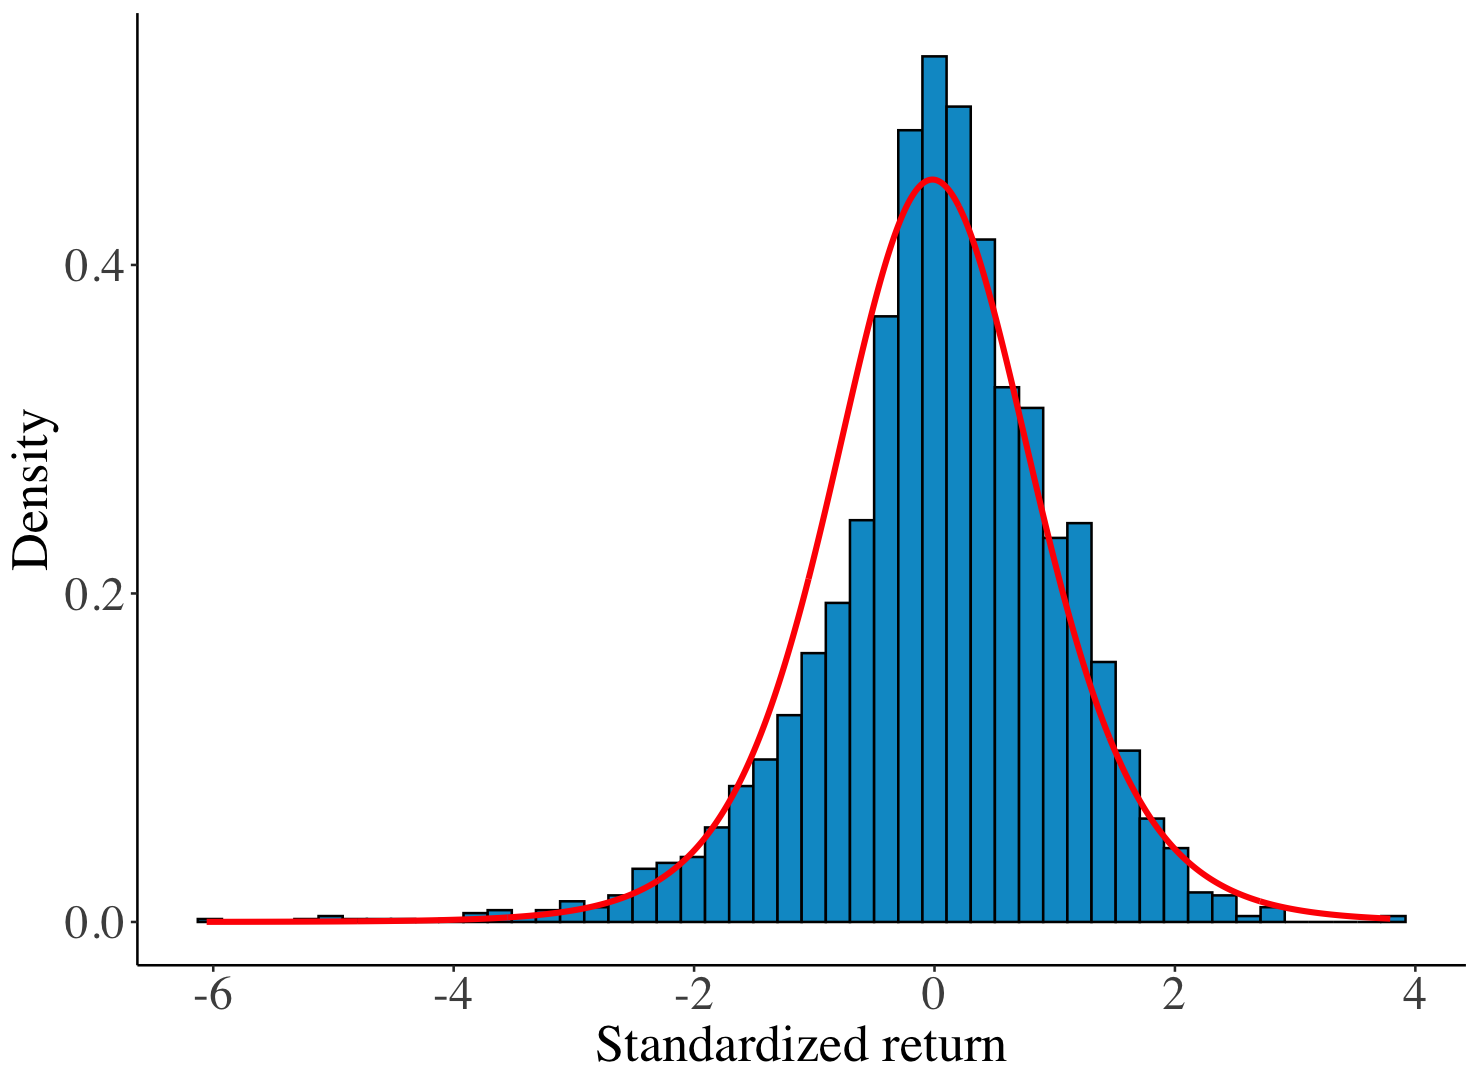
\includegraphics[scale=0.17]{../../plots/3.5.png} % Replace 
    \caption{Histogram of standardized returns with the fitted asymmetric $t$-distribution, GARCH(1,1).}
    \label{3.5}
\end{figure}

\begin{figure}[H]
    \centering
    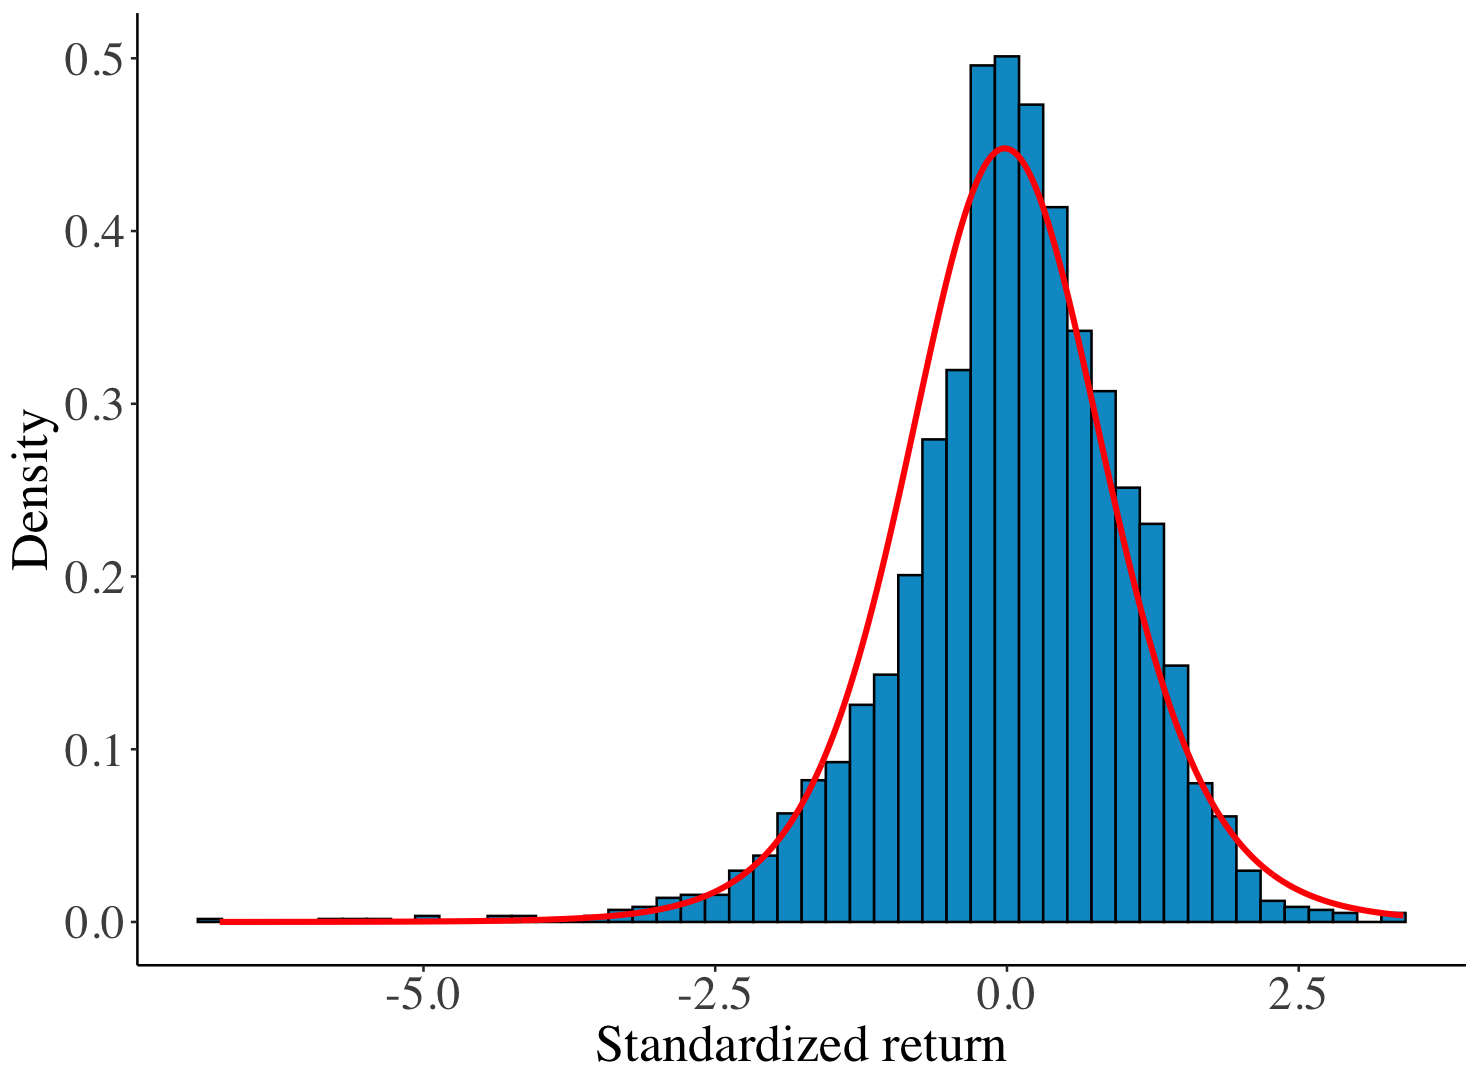
\includegraphics[scale=0.17]{../../plots/3.6.png} % Replace 
    \caption{Histogram of standardized returns with the fitted asymmetric $t$-distribution, GJR-GARCH(1,1).}
    \label{3.6}
\end{figure}

The Q–Q plots shown in Figures~\ref{3.7} and~\ref{3.8} further confirm that the asymmetric $t$-distribution provides a better fit to the standardized returns than the normal distribution. Nevertheless, the left tail of the empirical distribution remains inadequately modeled, exhibiting significantly heavier tails than those captured by the asymmetric $t$-distribution. Additionally, the comparisons between the empirical cumulative distribution functions (CDF) and their theoretical counterparts in Figures~\ref{3.9} and~\ref{3.10} reinforce the conclusion that the asymmetric $t$-distribution performs reasonably well in fitting the standardized returns.

Parametric models attempting to fit the full distribution are inevitably influenced by the high density of observations around the center, which may reduce their accuracy in capturing extreme values. For risk management, this is particularly concerning, as it risks underestimating the severity and likelihood of extreme negative returns. The inadequately modeled left tail demands special attention; thus, extreme value theory, which explicitly targets tail behavior, is introduced in the next approach. 

\begin{figure}[H]
    \centering
    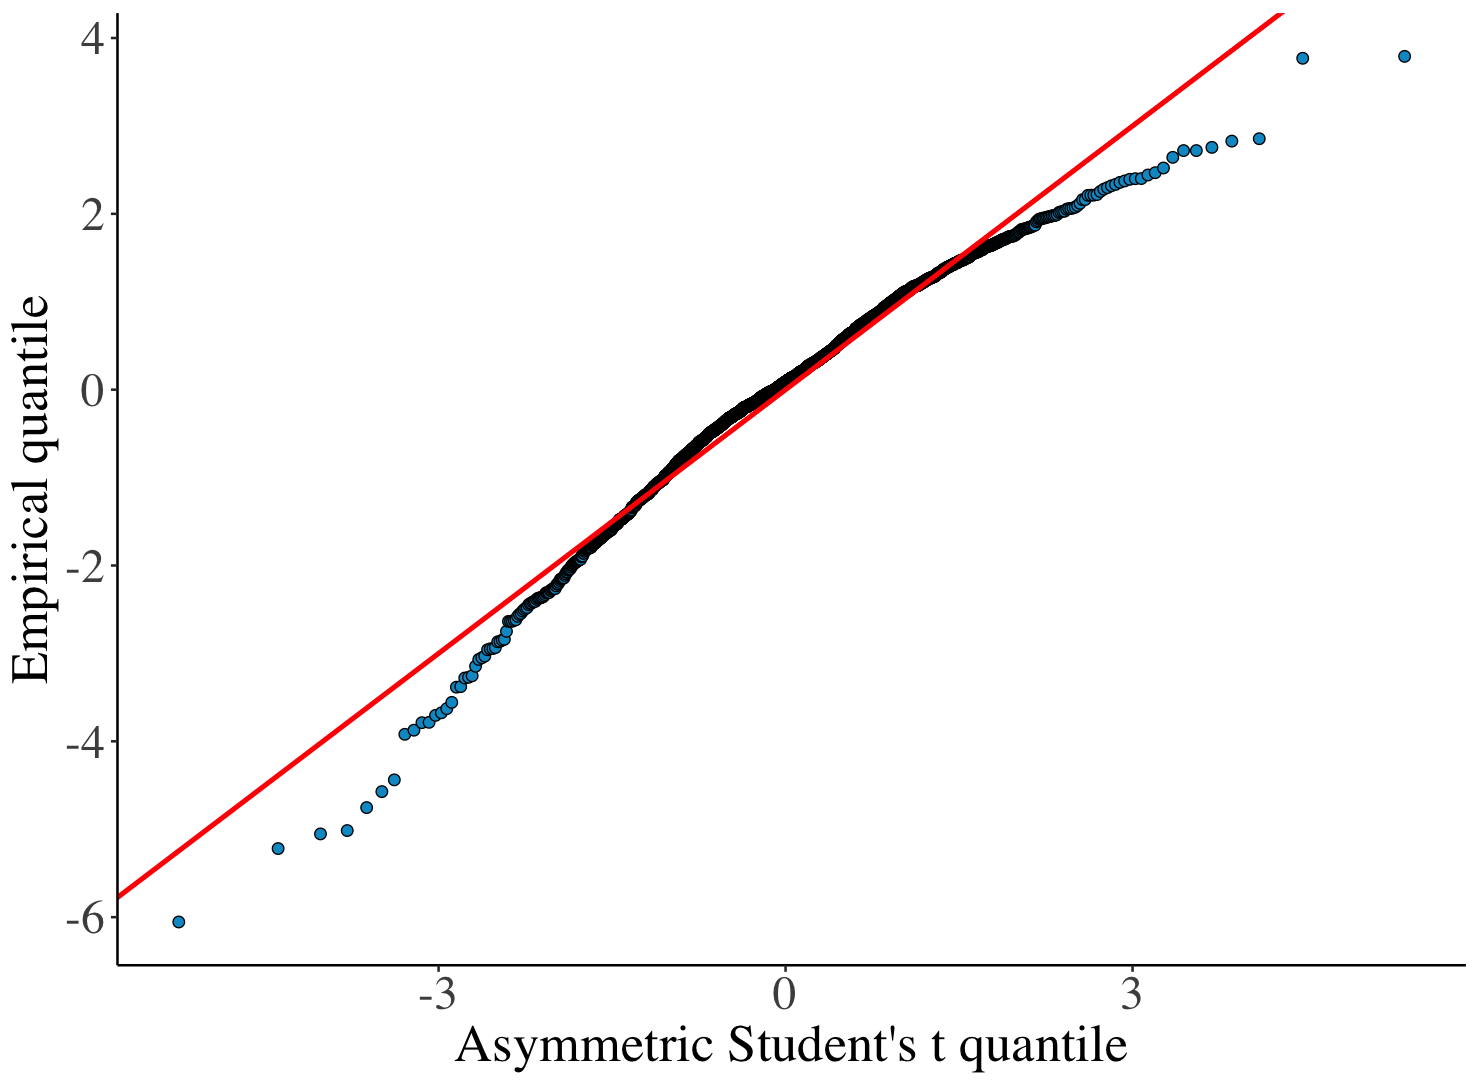
\includegraphics[scale=0.17]{../../plots/3.7.png} % Replace 
    \caption{QQ plot of standardized returns against the asymmetric $t$-distribution, GARCH(1,1).}
    \label{3.7}
\end{figure}

\begin{figure}[H]
    \centering
    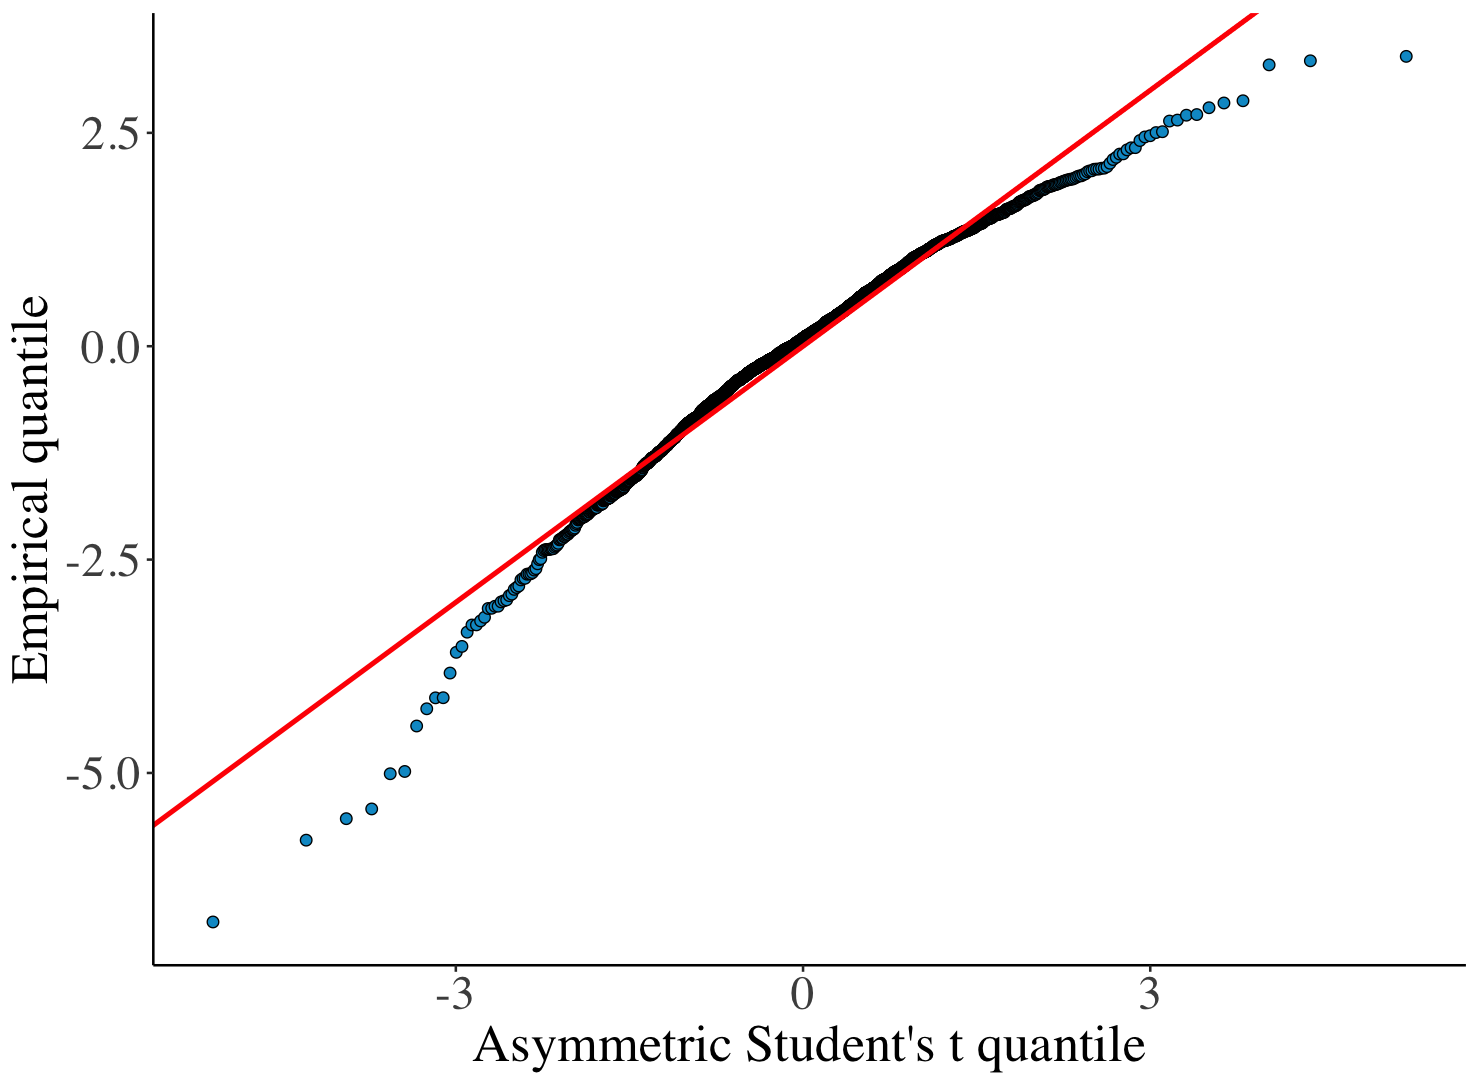
\includegraphics[scale=0.17]{../../plots/3.8.png} % Replace 
    \caption{QQ plot of standardized returns against the asymmetric $t$-distribution, GJR-GARCH(1,1).}
    \label{3.8}
\end{figure}

\begin{figure}[H]
    \centering
    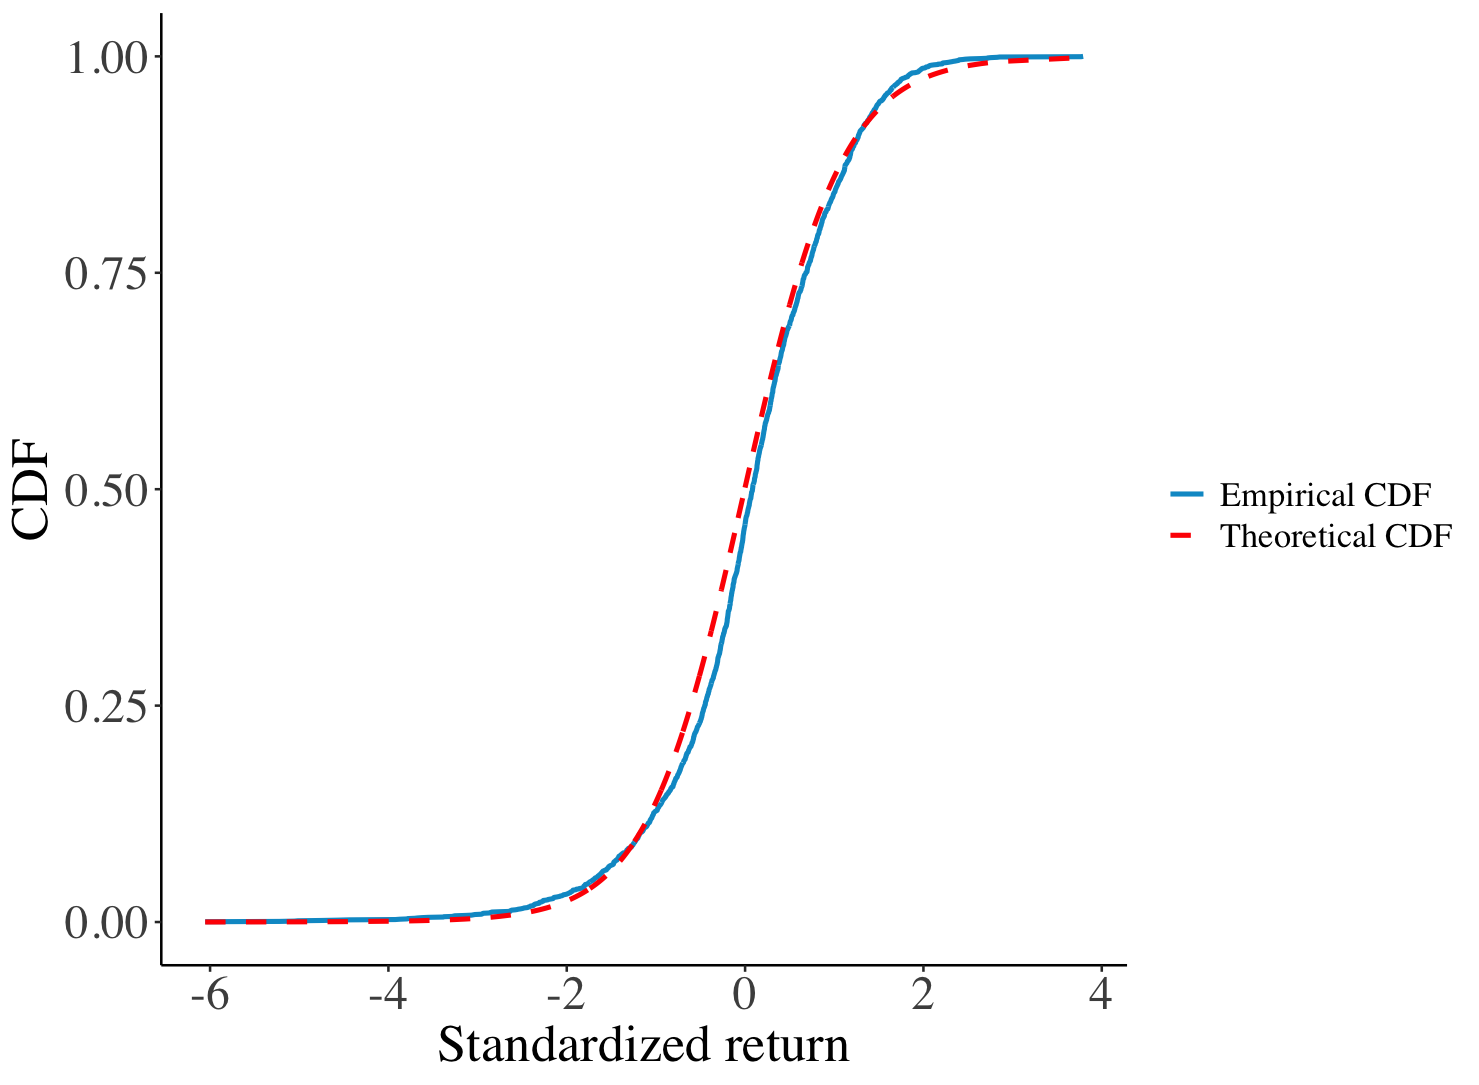
\includegraphics[scale=0.17]{../../plots/3.9.png} % Replace 
    \caption{Emprical CDF and theoretical asymmetric Student's $t$ CDF of standardized returns, GARCH(1,1).}
    \label{3.9}
\end{figure}

\begin{figure}[H]
    \centering
    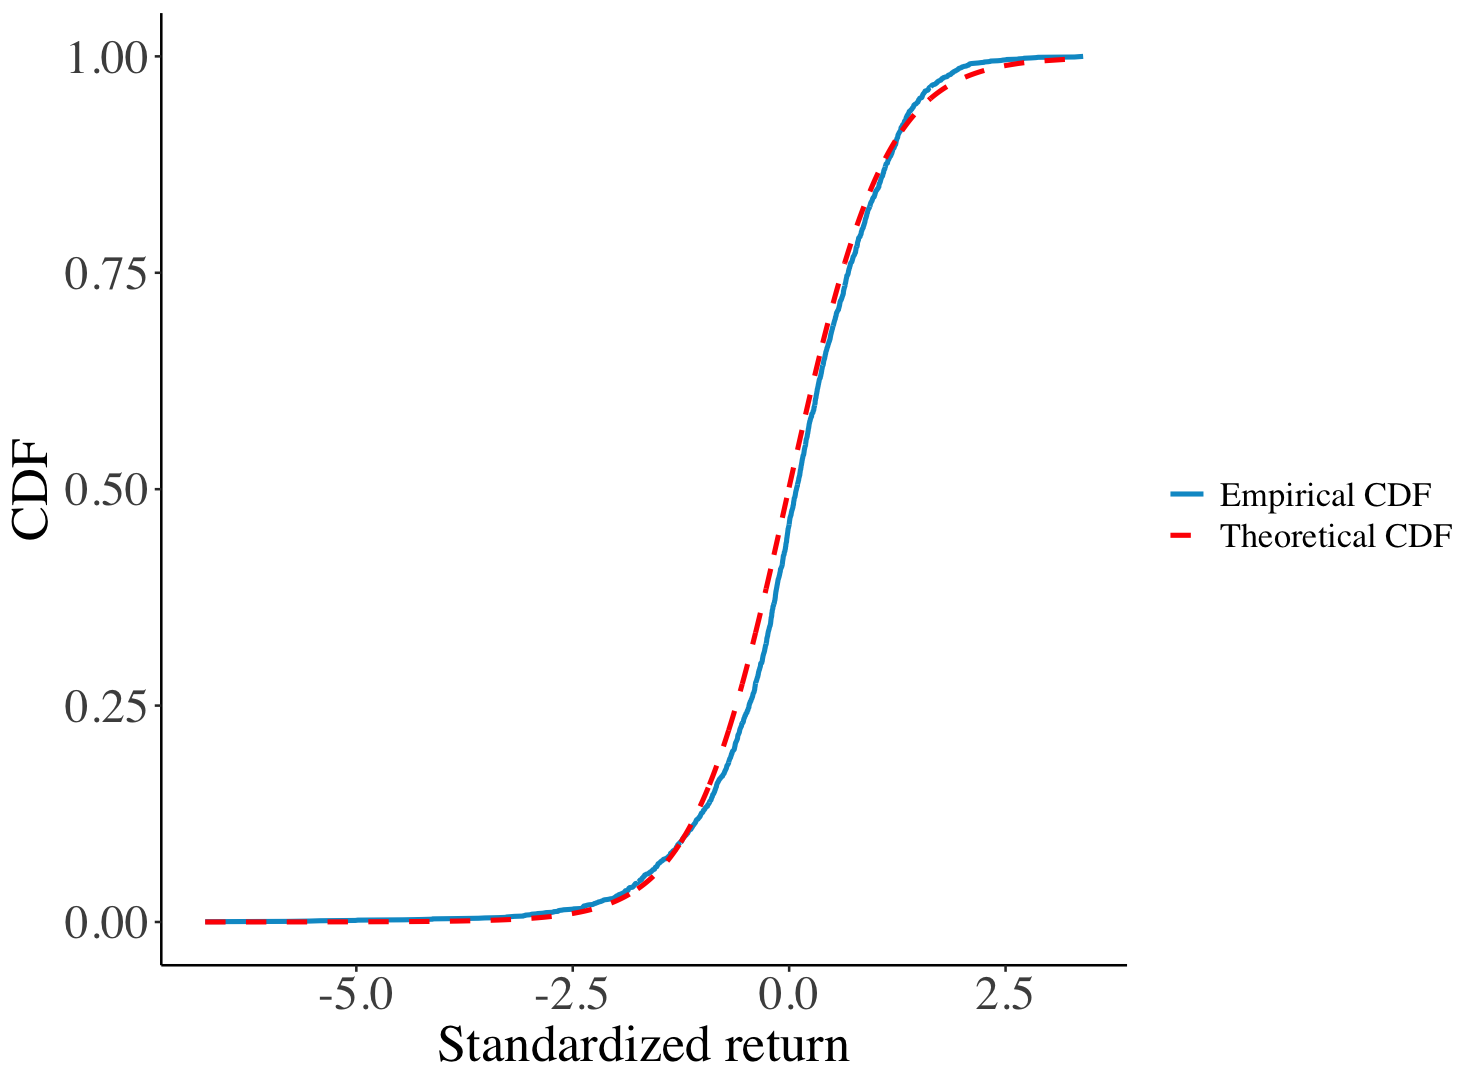
\includegraphics[scale=0.17]{../../plots/3.10.png} % Replace 
    \caption{Emprical CDF and theoretical asymmetric Student's $t$ CDF of standardized returns, GJR-GARCH(1,1).}
    \label{3.10}
\end{figure}

As noted by \citeA{Christoffersen2012}, the greatest risk to a portfolio arises from the sudden occurrence of a single large negative return. Therefore, explicit knowledge of the probabilities associated with such extreme events is central to financial risk management. Accurately modeling the left tail of the return distribution is thus critically important. Fortunately, a branch of statistics specifically addresses the modeling of these extreme events—extreme value theory (EVT).

Virtually all results in extreme value theory assume data to be independently and identically distributed (i.i.d.). Therefore, to apply this approach, the analysis is performed on standardized returns, which are assumed to meet the i.i.d. condition.

\newpage
The theoretical foundation of the approach considered here is provided by the Pickands–Balkema–de Haan theorem. This theorem states that, for a wide class of distributions $X \sim F$, given a sufficiently high threshold $u$, the conditional distribution of excesses $(X - u)$, given $X > u$, can be approximated by a generalized Pareto distribution (GPD). For a detailed statement and an outline of the proof, see \cite{Cont2001}. Consequently, the GPD naturally arises as a suitable model for the conditional tail distribution of returns, as emphasized by \citeA{Tsay2010}. Although the theorem is originally stated for the right tail, modeling the left tail simply involves applying the theorem to the negative of the returns (multiplying returns by -1).

This methodology, rooted in the Pickands–Balkema–de Haan theorem, is known in the extreme value literature as the peak-over-threshold (POT) approach. For alternative EVT-based approaches tailored specifically to financial returns, readers are referred to the chapters on extreme value theory in \citeA{Tsay2010} and \citeA{Christoffersen2012}. Further applications of EVT to financial risk management are discussed by \citeA{mcneil1999}. The particular implementation considered here was introduced by \citeA{mcneil2000estimation}.

For negative standardized returns, define $y_{t+1} = -z_{t+1}$. Then, the conditional PDF for observations exceeding a threshold $u$ is given by:
\begin{equation}
f(y; \xi, \beta, u | y>u) =
\begin{cases}
\dfrac{1}{\beta} \left(1 + \dfrac{\xi(y - u)}{\beta} \right)^{-\left(1 + \frac{1}{\xi}\right)}, & \text{for } \xi \ne 0, \; y \ge u \text{ if } \xi > 0,\; \\ & u \leq y \leq u- \frac{\sigma}{\xi} \text{ if } \xi < 0 ;\\
\\
\dfrac{1}{\beta} \exp\left(-\dfrac{y - u}{\beta}\right), & \text{for } \xi = 0,\; y \geq u.
\end{cases}
\label{eq:3.5}
\end{equation}

In the above expression, $\xi$ is the tail-index parameter, which controls the tail’s heaviness. Because financial returns exhibit tails heavier than those of the normal distribution, only the case $\xi > 0$ is considered here. In this scenario, the conditional PDF simplifies to:
\[
f(y; \xi, \beta, u | y>u) =
\dfrac{1}{\beta} \left(1 + \dfrac{\xi(y - u)}{\beta} \right)^{-\left(1 + \frac{1}{\xi}\right)}, \text{ for } \xi \ge 0, \; y \ge u.
\]

The second complete univariate model is therefore defined as:
\begin{equation}
\begin{aligned}
R_{t+1} &= \sigma_{t+1} z_{t+1}, \quad \text{where } z_{t+1} \sim \text{i.i.d. } D(0,1), \\
&\quad \quad  \quad  \quad  \quad  \quad \ \text{with } -z_{t+1} \mid (-z_{t+1} > u) \sim \text{GPD}(\xi, \beta, u),
\end{aligned}
\label{eq:3.6}
\end{equation}
and where the conditional variance $\sigma^2_{t+1}$ follows either a GARCH(1,1) or GJR-GARCH(1,1) specification.

For parameter estimation, the approach of \citeA{mcneil2000estimation} is followed. In the first step, the parameters of the volatility specification are estimated using quasi-maximum likelihood. In the second step, the parameters of the GPD are estimated via maximum likelihood using the standardized returns. \citeA{Christoffersen2012} discusses alternative estimation methods, including a semiparametric approach that is popular in the literature: the Hill estimator for the tail index $\xi$.

Before estimating the model, a threshold $u$ must be selected. As noted by \citeA{Christoffersen2012}, the choice of $u$ involves a trade-off between bias and variance: a high threshold is supported by extreme value theory but may result in too few observations, increasing variance; conversely, a low threshold provides more data but may lead to overfitting and to model misspecification by fitting observations outside the tail region. Discussions on the selection of $u$ can be found in \citeA{Tsay2010} and \citeA{coles2001}. \footnote{\citeA{Christoffersen2012} also suggests selecting $u$ by identifying the point at which the tail begins to depart from normality in the QQ plot of standardized residuals, and recommends using at least 50 observations in the tail fit, based on evidence from simulation studies.}

Fortunately, a useful property of the generalized Pareto distribution can guide this choice. For any $u > u_0$, where $u_0$ is a threshold above which the GPD provides a valid approximation, the mean excess function $e(u) = \mathbb{E}[y - u \mid y > u]$ is linear in $u$. Thus, plotting the empirical mean excess function over a range of threshold values allows identification of the region where the function becomes approximately linear—indicating a suitable choice for $u$. Figures~\ref{3.11} and~\ref{3.12} suggest that choosing $u \geq 1.8$ is reasonable for both sets of standardized returns.

\begin{figure}[H]
    \centering
    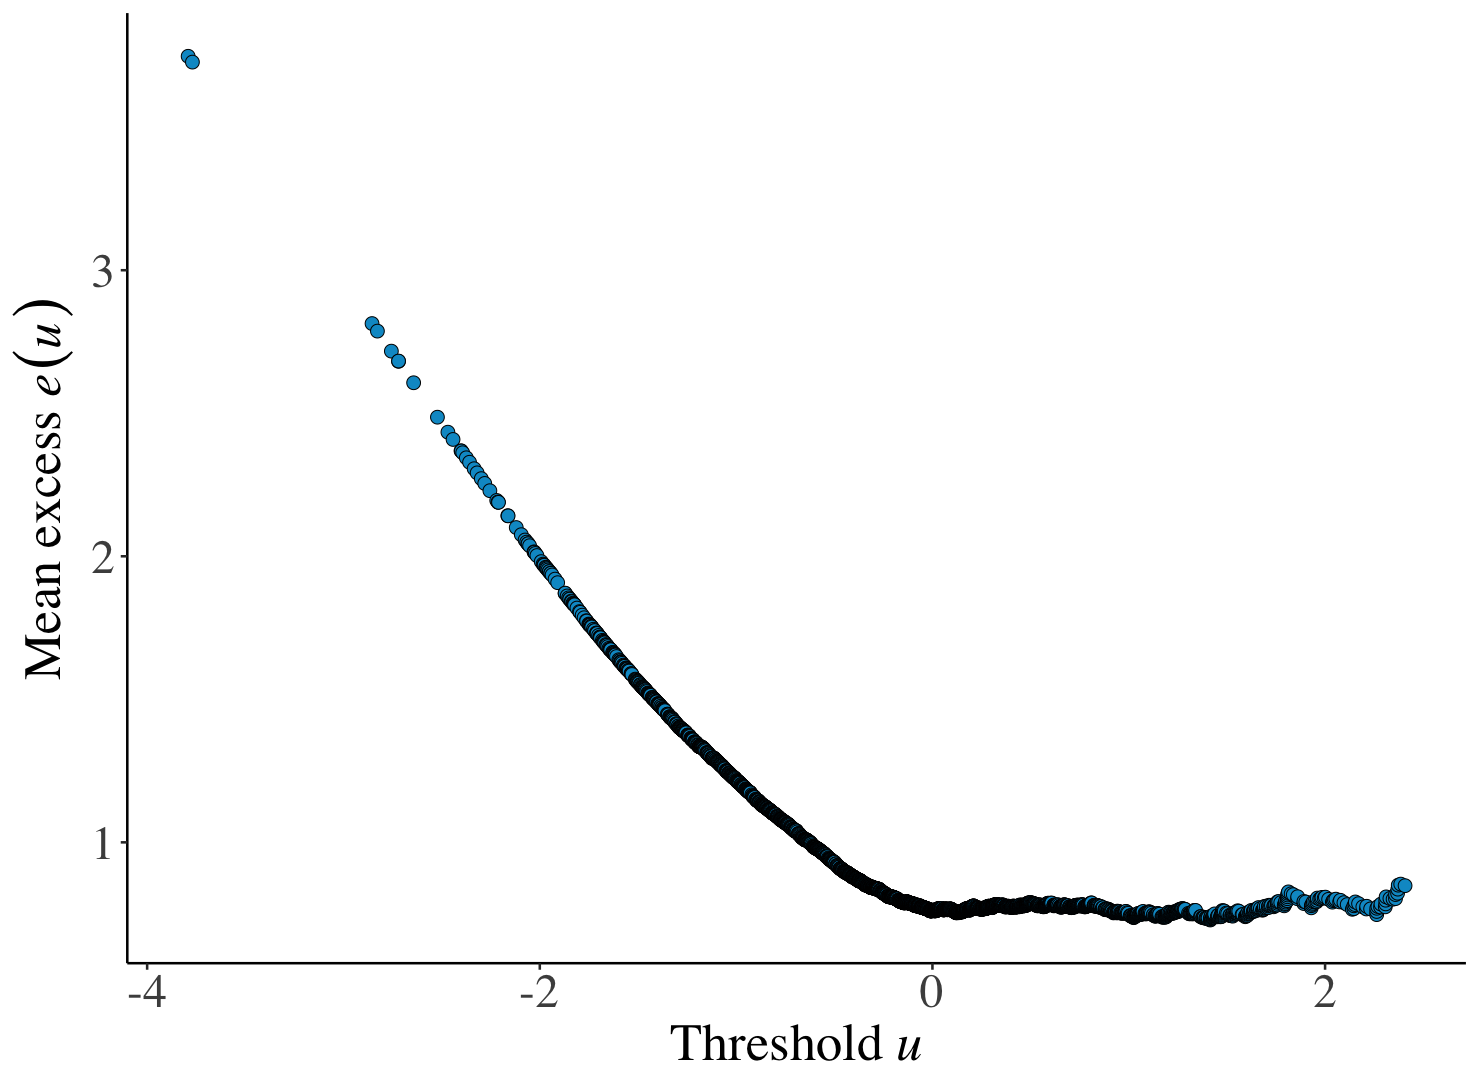
\includegraphics[scale=0.18]{../../plots/3.11.png} % Replace 
    \caption{Mean excess function $e(u)$, GARCH(1,1).}
    \label{3.11}
\end{figure}

\begin{figure}[H]
    \centering
    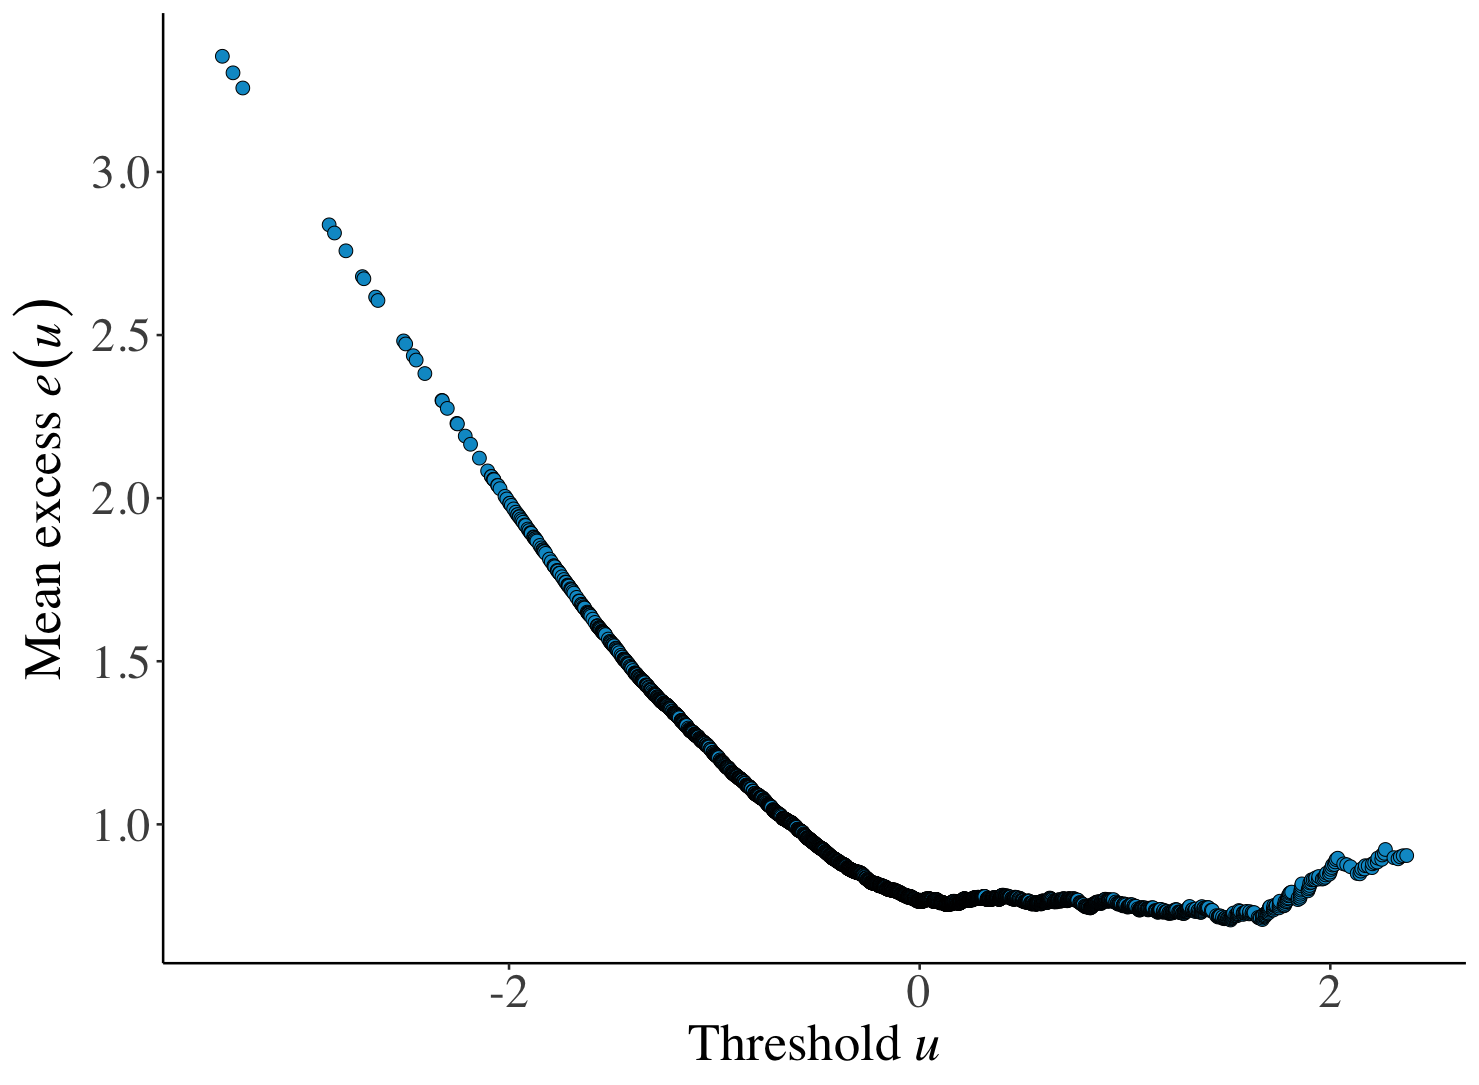
\includegraphics[scale=0.18]{../../plots/3.12.png} % Replace 
    \caption{Mean excess function $e(u)$, GJR-GARCH(1,1).}
    \label{3.12}
\end{figure}

Setting $u = 1.8$, the model in Equation~\eqref{eq:3.4} can be estimated (with the resulting GPD parameters $\beta_{\text{GPD}}$ and $\xi$ for both fits reported in Table~\ref{tab:3.1}), and the goodness-of-fit can be assessed visually. Figures~\ref{3.13} and~\ref{3.14} show that, for both sets of standardized returns—GARCH(1,1) and GJR-GARCH(1,1), respectively—the GPD provides a reasonable fit to the left tail.\footnote{The plots show the quantiles of the excesses over the threshold, along with the fitted GPD starting at zero, to aid in the visual assessment.}  However, some nuances remain, as the model’s ability to capture the tail behavior tends to diminish further into the extreme tail. To complement the visual assessment, Figures~\ref{3.15} and~\ref{3.16} display the empirical and theoretical cumulative distribution functions for both sets of standardized returns.

\begin{figure}[H]
    \centering
    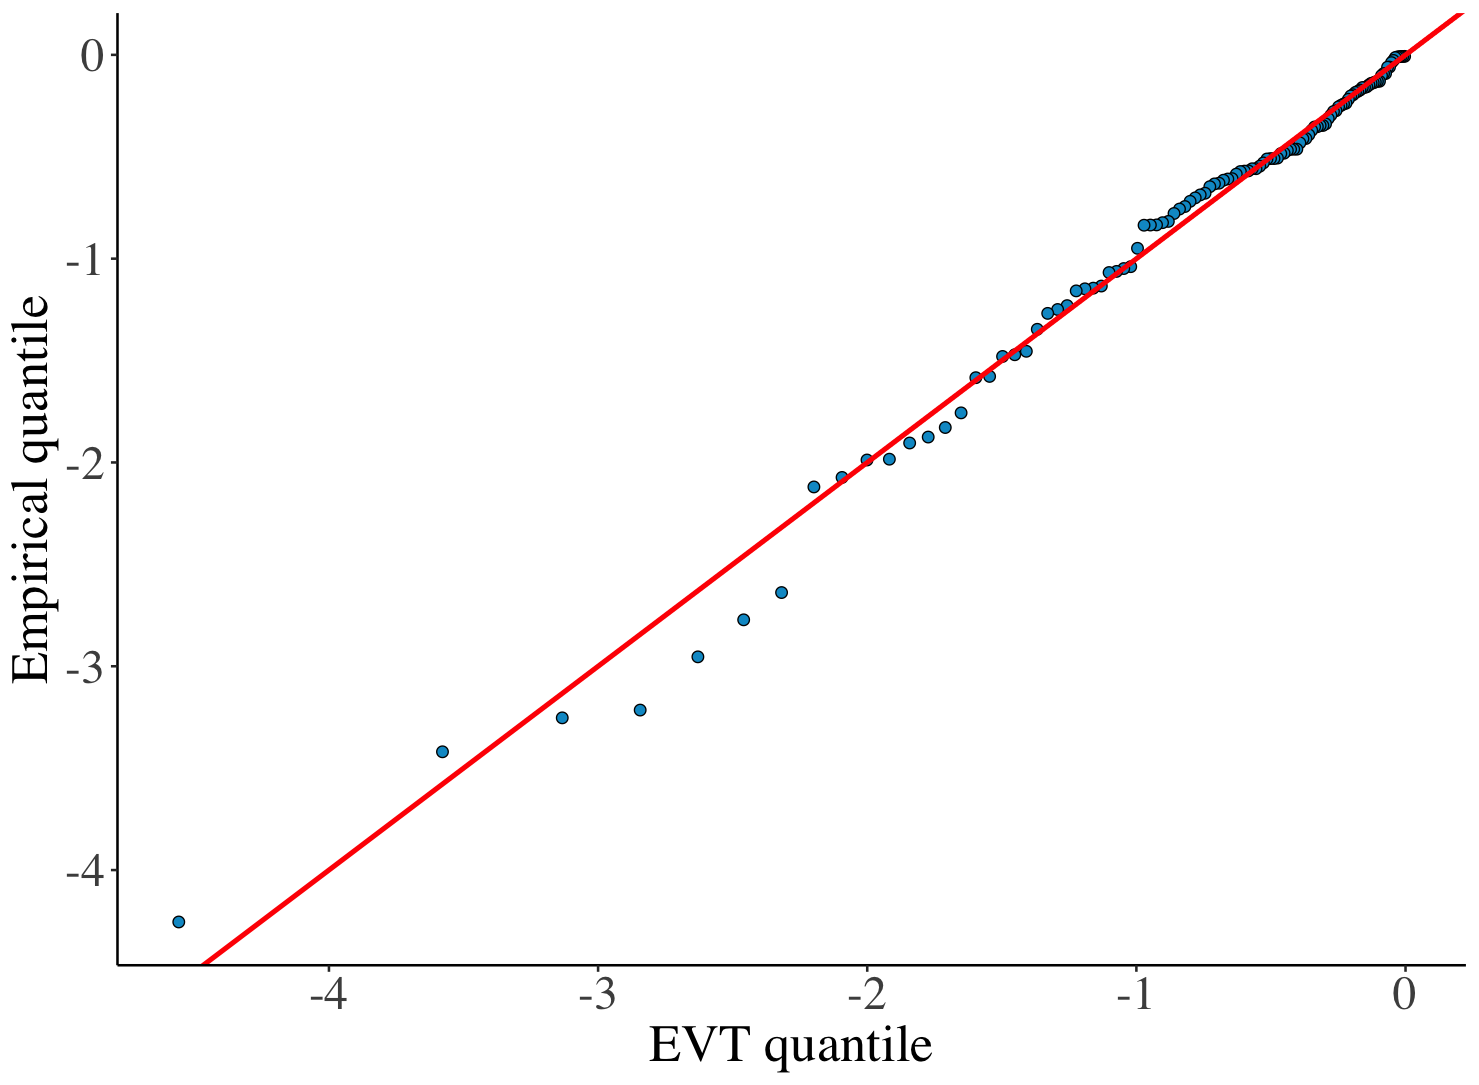
\includegraphics[scale=0.17]{../../plots/3.13.png} % Replace 
    \caption{QQ plot of standardized returns against the generalized Pareto distribution, GARCH(1,1).}
    \label{3.13}
\end{figure}

\begin{figure}[H]
    \centering
    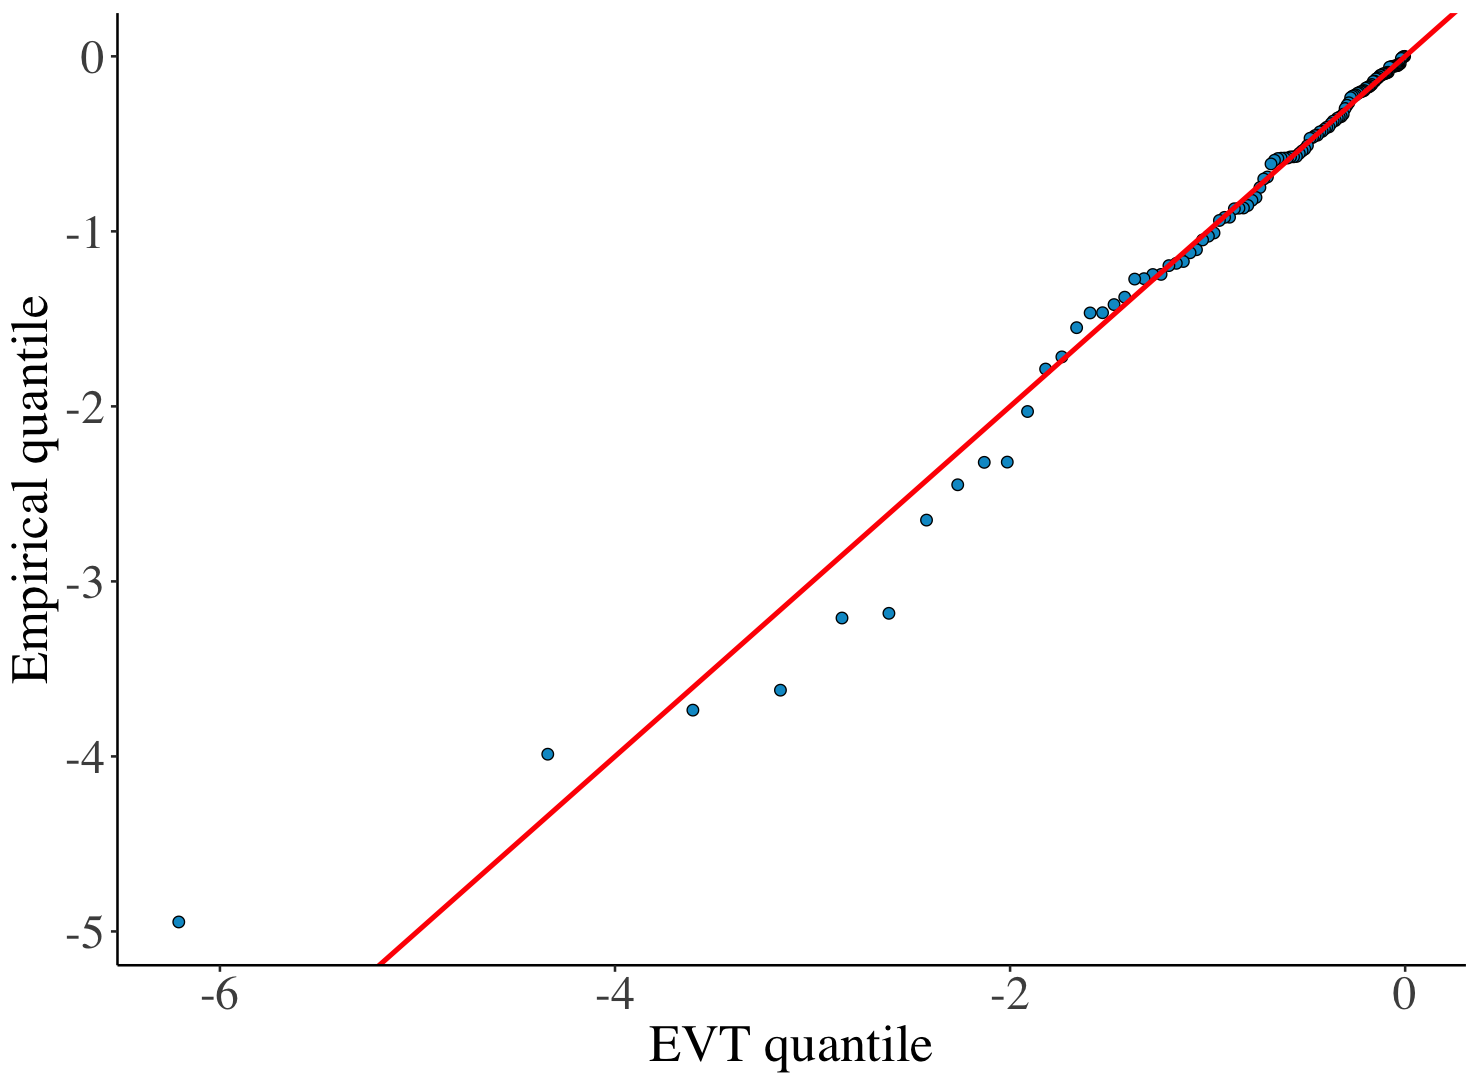
\includegraphics[scale=0.17]{../../plots/3.14.png} % Replace 
    \caption{QQ plot of standardized returns against the generalized Pareto distribution, GJR-GARCH(1,1).}
    \label{3.14}
\end{figure}

\begin{figure}[H]
    \centering
    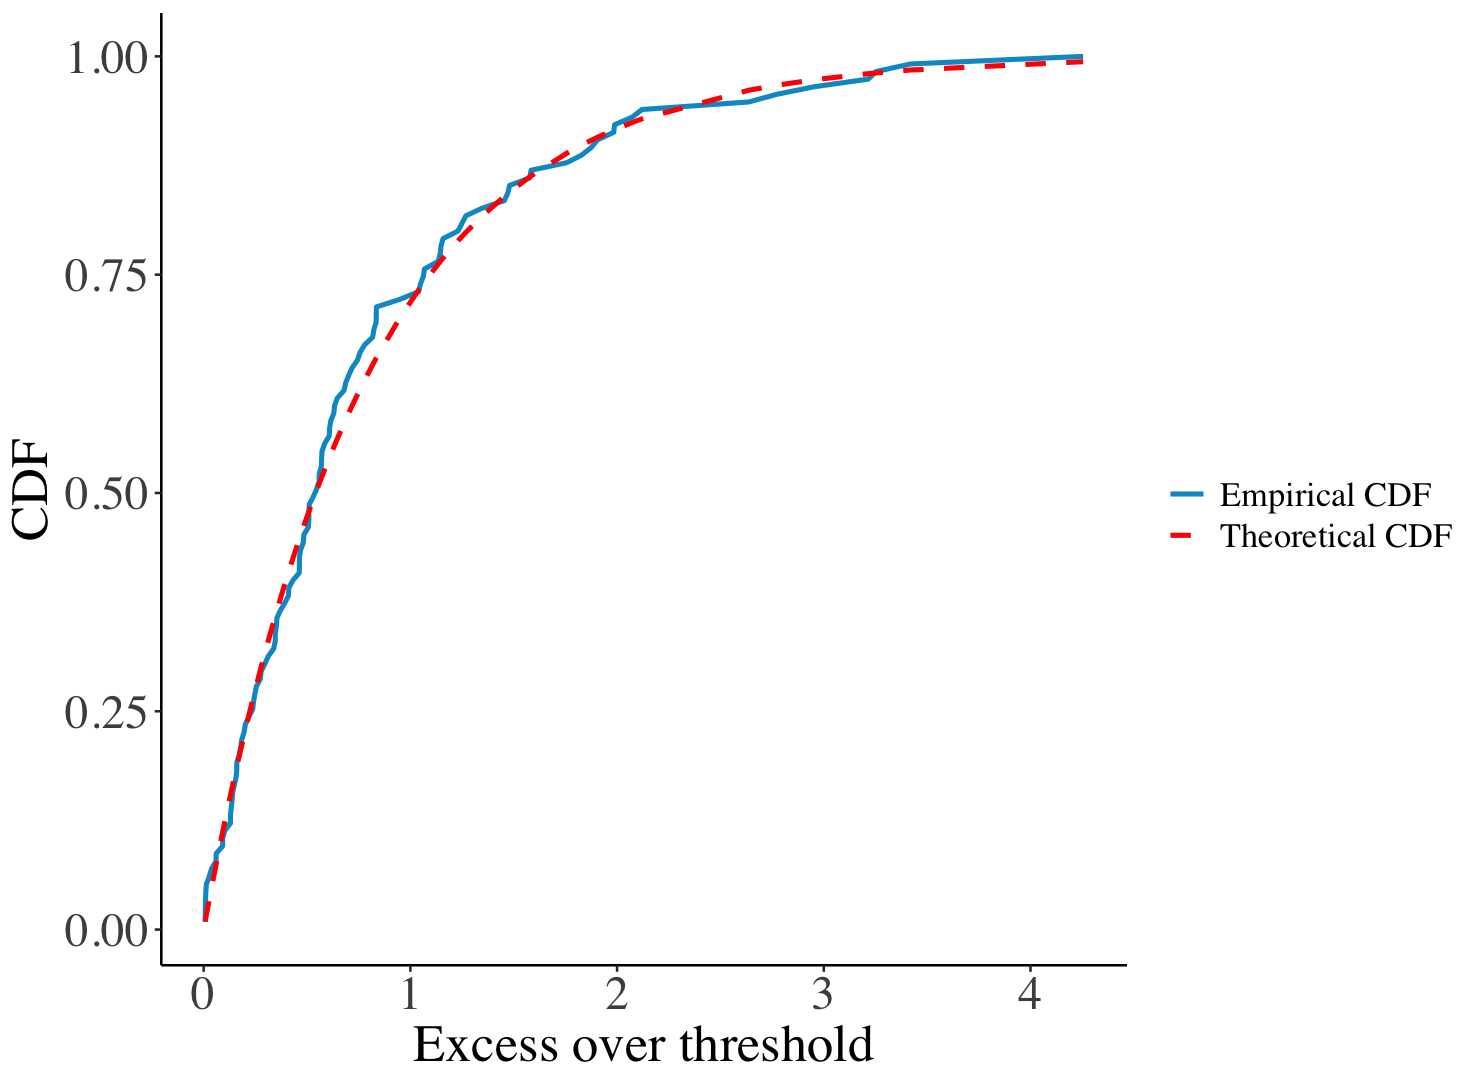
\includegraphics[scale=0.17]{../../plots/3.15.png} % Replace 
    \caption{Empirical CDF and theoretical EVT CDF of standardized returns, GARCH(1,1).}
    \label{3.15}
\end{figure}

\begin{figure}[H]
    \centering
    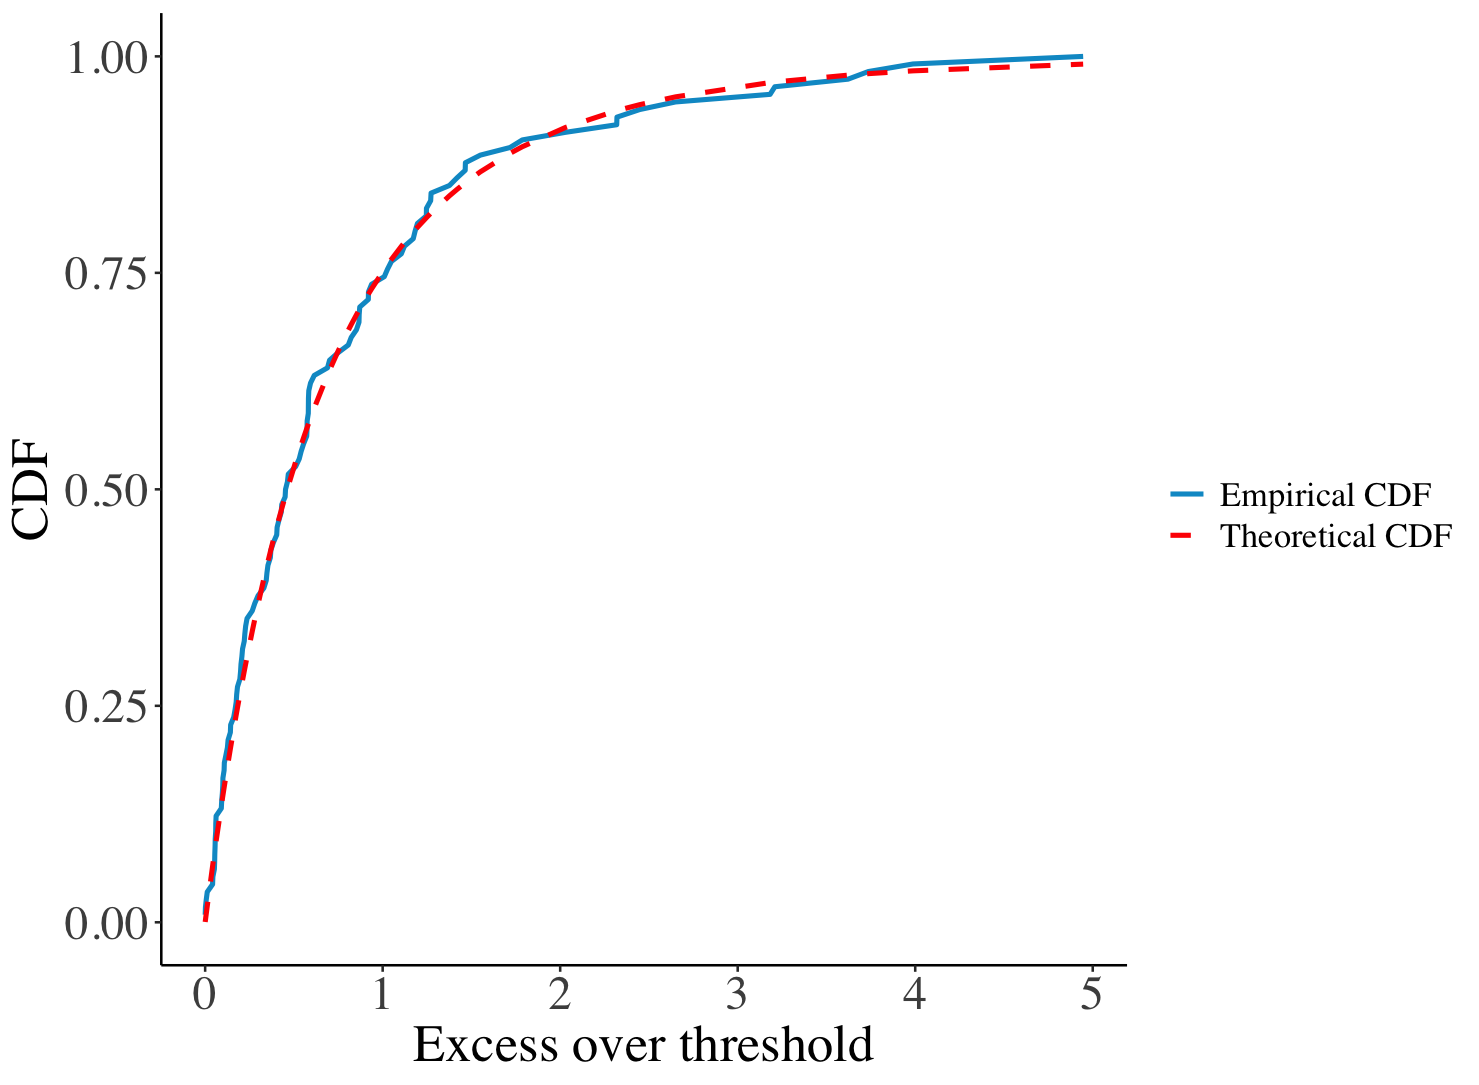
\includegraphics[scale=0.17]{../../plots/3.16.png} % Replace 
   \caption{Empirical CDF and theoretical EVT CDF of standardized returns, GJR-GARCH(1,1).}
    \label{3.16}
\end{figure}

This chapter concludes by summarizing the two approaches explored for modeling the standardized returns: the asymmetric Student’s $t$-distribution and the peak-over-threshold method derived from extreme value theory. The former is a full-distribution model aimed at capturing the entire range of return behavior, while the latter focuses exclusively on the left tail to address the shortcomings of the full-distribution approach in modeling extreme losses. In essence, the first approach provides a complete density specification, whereas the second concentrates solely on tail behavior.

The variance parameters were estimated via QMLE, after which the focus shifted to the standardized returns. In total, four models for returns were considered. Table \ref{tab:3.1} reports the estimated parameters for each model.

\begin{table}[htbp]
\footnotesize
\centering
\begin{tabular}{lcccccccc}
\toprule
\textbf{Model} & $\omega$ & $\alpha$ & $\beta$ & $\theta$ & $d_1$ & $d_2$ & $\beta_{\text{GPD}}$ & $\xi$ \\
\midrule
GARCH-Asyt &  $3.9\mathrm{e}{-6}$ & 0.171 &  0.794 & - & 7.35 & 0.0115 & - & -\\
GJR-Asyt & $4.0\mathrm{e}{-6}$ & 0.054 &  0.795 & 4.62 & 7.83 &  0.0129 & - & -\\
GARCH-EVT &  $3.9\mathrm{e}{-6}$ & 0.171 &  0.794 & - & - & - & 0.774 & 0.029 \\
GJR-EVT & $4.0\mathrm{e}{-6}$ & 0.054 &  0.795 & 4.62 & - & - & 0.621 & 0.206\\
\bottomrule
\end{tabular}
\caption{Estimated parameters.}
\label{tab:3.1}
\end{table}

In the next section, the models will be used for forecasting and evaluated from both a statistical and a risk management perspective.

\newpage
\newpage
\chapter{Forecasting and Evaluation}
\label{chap:4}

The next step is to use the models constructed in the previous chapters for forecasting and to evaluate their performance. George E. P. Box is famously quoted as saying, \textit{“All models are wrong, but some are useful.”} In light of Box’s observation, the task now is to evaluate whether the models constructed are among those that are useful. The evaluation will proceed from two perspectives: a statistical perspective to assess model validity, and a risk management perspective to assess their practical usefulness.

To recap and introduce the forecasting procedure, the model parameters were estimated using S\&P 500 log returns from January 2014 to December 2024. The fitted models were then used to forecast the one-day-ahead variance and return density from January to April 2025. To assess their usefulness in a risk management context, the one-day-ahead Value at Risk (VaR) and Expected Shortfall (ES) are computed based on the forecasts from the fitted models.\footnote{Following standard risk-management convention, VaR and ES are reported as positive quantities representing the magnitude of a potential loss, even though the underlying returns in the loss tail are negative. This is why the formal definitions introduced later in the chapter carry a leading minus sign in front of the return quantile and tail expectation.}

As noted by \citeA{Christoffersen2012}, before using the variance model for forecasting, it is appropriate to subject the estimated model to diagnostic checks. In \hyperref[chap:1]{Chapter 1}, the dependence between squared returns was illustrated via the autocorrelation function (ACF) of squared returns. One of the primary objectives of volatility modeling is to eliminate this dependence structure by constructing a volatility measure, $\sigma^2_{t+1}$, such that the standardized squared returns, $\frac{R^2_{t+1}}{\sigma^2_{t+1}}$, exhibit no systematic autocorrelation patterns.

Figures~\ref{4.1} and~\ref{4.2} display the ACFs of the standardized squared returns (2014-2024) under the GARCH(1,1) and GJR-GARCH(1,1) models, respectively. It can be observed that the dependence structure seen in \hyperref[chap:1]{Chapter 1} has now disappeared, indicating that the GARCH models have been effective at removing the systematic autocorrelation patterns in the squared returns.

\begin{figure}[H]
    \centering
    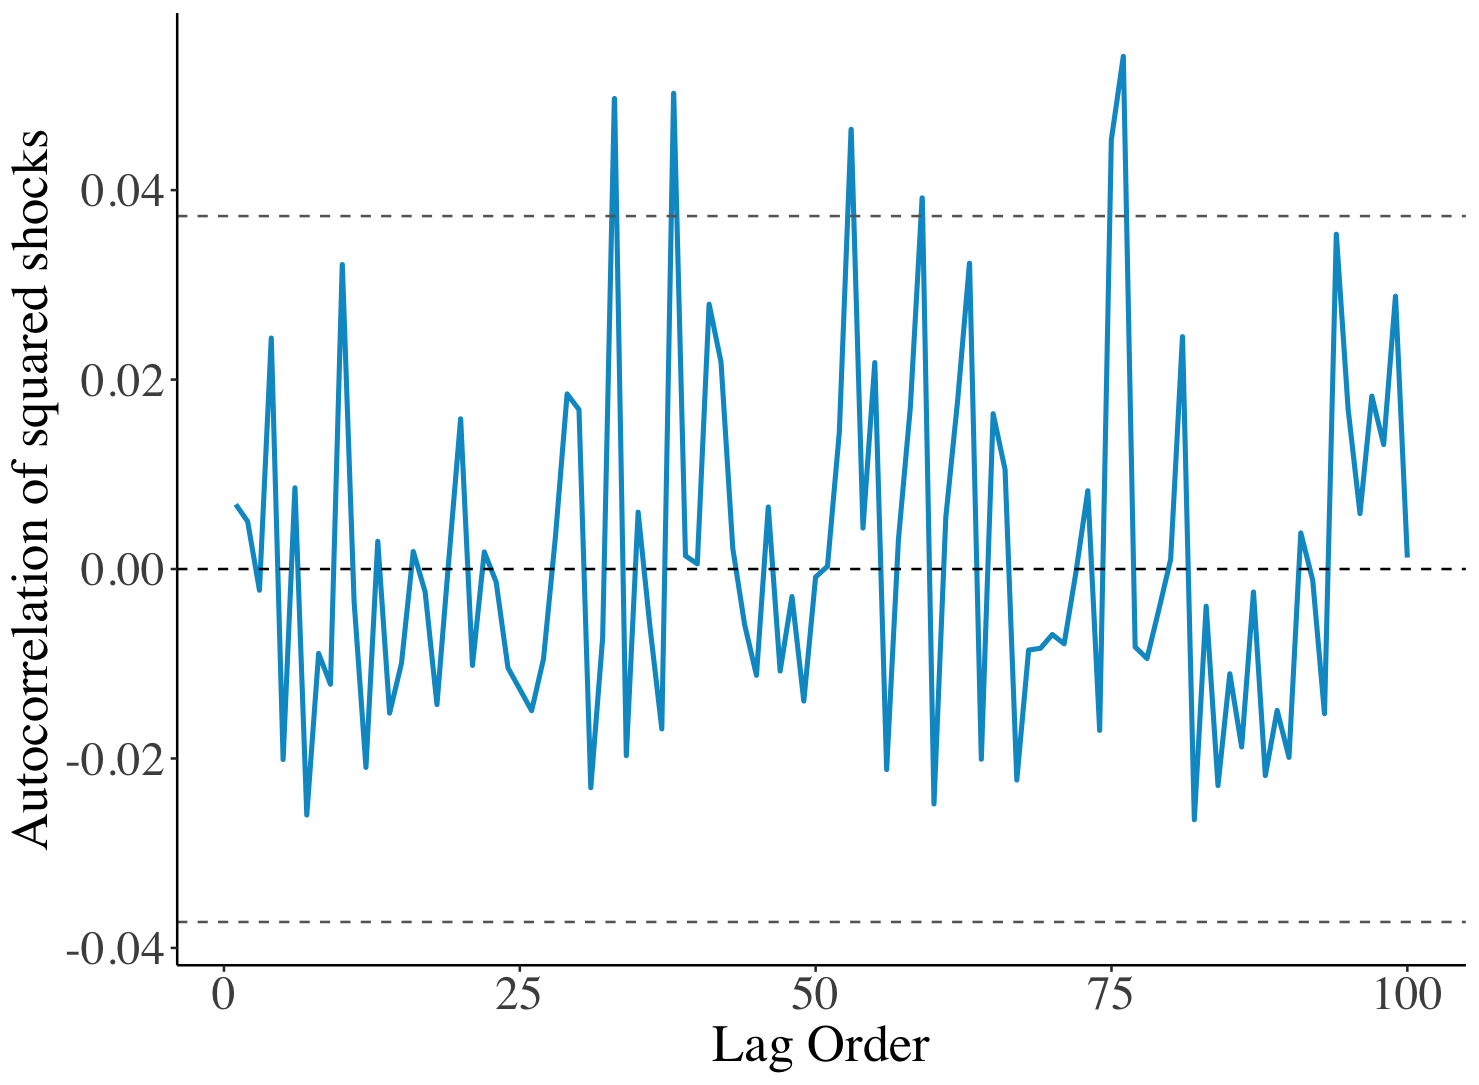
\includegraphics[scale=0.17]{../../plots/4.1.png} % Replace 
   \caption{Autocorrelation of squared returns over variance (2014-2024), GARCH(1,1).}
    \label{4.1}
\end{figure}

\begin{figure}[H]
    \centering
    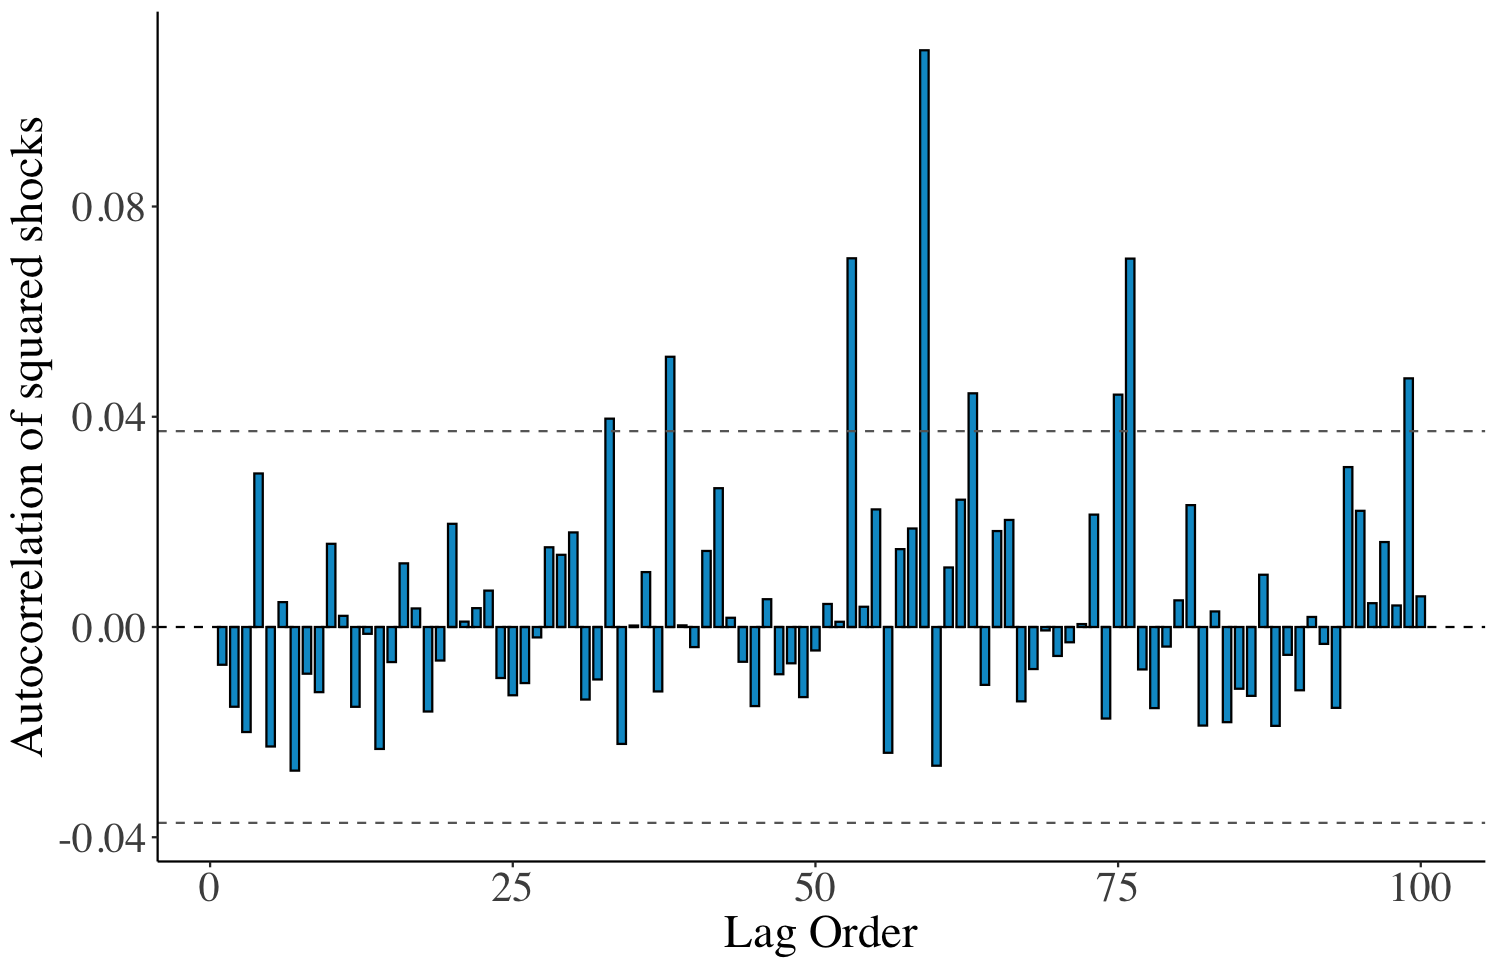
\includegraphics[scale=0.17]{../../plots/4.2.png} % Replace 
   \caption{Autocorrelation of squared returns over variance (2014-2024), GJR-GARCH(1,1).}
    \label{4.2}
\end{figure}

To complement the visual evidence, a Ljung–Box test was performed on the squared standardized residuals of both models using $m=7$ lags. The resulting $p$-values are 0.6528 for the GARCH(1,1) model and 0.3485 for the GJR-GARCH(1,1) model. In both cases, the null hypothesis that the first seven autocorrelations are jointly zero cannot be rejected. These results support the conclusion suggested by Figures~\ref{4.1} and~\ref{4.2}: the dependence structure originally present in squared returns has been effectively removed by the volatility models.

Before proceeding to forecasting, it is useful to assess which model performs better on the training set (2014–2024) under an appropriate loss function. When selecting a loss function, it is important to consider that risk managers may weigh positive and negative volatility forecast errors differently: underestimating volatility may be more costly than overestimating it by the same amount.

The QLIKE loss function addresses this asymmetry and is commonly used in the literature to evaluate volatility models, see \citeA{elliott201}. The QLIKE loss function is defined as:

\begin{equation}
\text{QLIKE}_t = \frac{R^2_{t+1}}{\sigma^2_{t+1}} - \ln\left(\frac{R^2_{t+1}}{\sigma^2_{t+1}}\right) - 1.
\label{eq:4.1}
\end{equation}

A loss function is said to be robust if the ranking of any two volatility forecasts is the same when using an observed volatility proxy as when (hypothetically) using the unobserved true volatility, as defined by \citeA{patton2011}. Robustness is clearly a desirable property for a volatility forecast loss function, and \citeA{patton2011} shows that the QLIKE loss function possesses this quality.

The mean QLIKE over the training period for both volatility models is reported in Table~\ref{tab:4.1}. The results suggest that the GJR-GARCH model outperforms the standard GARCH(1,1) model during the training period.

\begin{table}[htbp]
\centering
\begin{tabular}{lc}
\toprule
\textbf{Model} & Mean QLIKE \\
\midrule
GARCH(1,1)&  1.6011  \\
GJR-GARCH(1,1) & 1.5673 \\
\bottomrule
\end{tabular}
\caption{Mean QLIKE over the training period}
\label{tab:4.1}
\end{table}

The volatility models considered here were constructed using squared returns as the volatility proxy. As noted by \citeA{Christoffersen2012}, squared returns are an unbiased but potentially very noisy proxy for conditional variance. Alternatives include realized variance and range-based measures, which possess valuable predictive power and other desirable statistical properties. Readers interested in models based on alternative volatility proxies are referred to \citeA{Christoffersen2012} and the references therein. When using intraday-based proxies, it is important to account for market microstructure effects. \citeA{Tsay2010} and \citeA{Campbell1997} provide overviews of the microstructure of financial markets.

A simple likelihood ratio (LR) test can also be used to assess whether the additional parameter in the GJR-GARCH model is statistically significant relative to the simpler GARCH(1,1) model. As noted by \citeA{Christoffersen2012}, the LR test provides a straightforward way to evaluate whether added parameters are statistically meaningful.

Consider two nested models with log-likelihood values $L_0$ and $L_1$, where model 0 is a special case of model 1. The models can be compared using the likelihood ratio statistic:

\begin{equation}
\text{LR} = 2\left( \ln(L_1) - \ln(L_0) \right).
\label{eq:4.2}
\end{equation}

Under the null hypothesis that the additional parameter(s) in model 1 are not significant, the LR statistic follows a chi-squared distribution with degrees of freedom equal to the number of parameters added. In this case, since GJR-GARCH(1,1) adds one parameter to GARCH(1,1), the degrees of freedom equal 1.

Using the asymmetric $t$-distribution as the likelihood function, the LR test yields a $p$-value below 1\%, indicating little evidence in the data in favor of the null hypothesis. Thus, the additional parameter in the GJR-GARCH model is statistically significant.

Forecasting begins by considering the first two models in Table~\ref{tab:3.1}, which combine the volatility models with the asymmetric $t$-distribution. These models forecast the entire density of the next day’s return, allowing for the computation of risk measures such as Value-at-Risk (VaR) and Expected Shortfall (ES). Following the definition in \citeA{Christoffersen2012}, VaR is a risk measure that answers the question: What is the loss that will only be exceeded $p \times 100\%$ of the time on the next trading day? In other words, VaR corresponds to a quantile of the distribution of tomorrow’s return.

Under the specification $R_{t+1} = \sigma_{t+1} z_{t+1}$, with $z_{t+1} \sim \text{i.i.d. asyt}(d_1, d_2)$, the 1-day ahead $p$-level VaR can be computed as:
\begin{equation}
\text{VaR}_{t+1}^p = -\sigma_{t+1} \, F^{-1}_{\text{asyt}}(p; d_1, d_2),
\label{eq:4.3}
\end{equation}
where
\[
F^{-1}_{\text{asyt}}(p; d_1, d_2) =
\begin{cases}
\dfrac{1}{B} \left[(1 - d_2) \sqrt{\dfrac{d_1 - 2}{d_1}} \, t^{-1}_{p/(1 - d_2)}(d_1) - A \right], & \text{if } p < \dfrac{1 - d_2}{2} \\
\dfrac{1}{B} \left[(1 + d_2) \sqrt{\dfrac{d_1 - 2}{d_1}} \, t^{-1}_{(p + d_2)/(1 + d_2)}(d_1) - A \right], & \text{if } p \geq \dfrac{1 - d_2}{2}.
\end{cases}
\]
Here, $t^{-1}_{q}(d)$ denotes the $q$-th quantile of the symmetric Student's $t$-distribution with $d$ degrees of freedom.

The 1-day ahead Expected Shortfall (ES) is defined as
$$\text{ES}_{t+1}^p=-\mathbb{E}[R_{t+1}|R_{t+1}<-\text{VaR}_{t+1}^p],$$ 
and under the assumption of the asymmetric $t$-distribution, it can be computed as:
\begin{equation}
\text{ES}_{t+1}^p = -\sigma_{\text{PF}, t+1} \, \text{ES}_{\text{asyt}}(p),
\label{eq:4.4}
\end{equation}
where
\[
\begin{aligned}
\text{ES}_{\text{asyt}}(p) &= \dfrac{C(1 - d_2)^2}{Bp}
\left[1 + \dfrac{1}{d_1 - 2} \left(\dfrac{BQ + A}{1 - d_2}\right)^2 \right]^{\frac{1 - d_1}{2}} \dfrac{d_1 - 2}{1 - d_1} \\
&\quad - \dfrac{AC(1 - d_2)}{Bp} \cdot \dfrac{\sqrt{\pi(d_1 - 2)}\, \Gamma\left(\frac{d_1}{2}\right)}{\Gamma\left(\frac{d_1 + 1}{2}\right)} \, t_{d_1}\left(\sqrt{\dfrac{d_1}{d_1 - 2}} \cdot \dfrac{BQ + A}{1 - d_2}\right),
\end{aligned}
\]
and $Q=F^{-1}_{\text{asyt}}(p; d_1, d_2)$.

According to \citeA{elliott201}, a density forecast—such as those produced by combining volatility models with the asymmetric $t$-distribution—should satisfy certain desirable properties. One of these is \textit{calibration}, which requires that if a density forecast assigns a specific probability to an event, then the event should occur with approximately that frequency over successive observations.

This property can be assessed using Value-at-Risk. At the $p = 2.5\%$ level, a well-calibrated model should produce VaR breaches approximately 2.5\% of the time during the evaluation period. Figures~\ref{4.3} and~\ref{4.4} show the daily returns of the S\&P 500 from January to April 2025, along with the one-day-ahead 2.5\% VaR forecasts and the corresponding VaR breaches, assuming an asymmetric $t$-distribution.

With 81 observations in the test period, approximately two breaches would be expected under correct coverage. However, both models exhibit more than two breaches, indicating a failure to meet the calibration criterion. It is also worth noting the dynamic and adaptive behavior of the VaR forecast: following the market shock induced by Trump’s tariff imposition, volatility increased sharply. The VaR initially fails to capture this rise—resulting in several breaches—but gradually adjusts to the new, higher volatility regime. 

\begin{figure}[H]
    \centering
    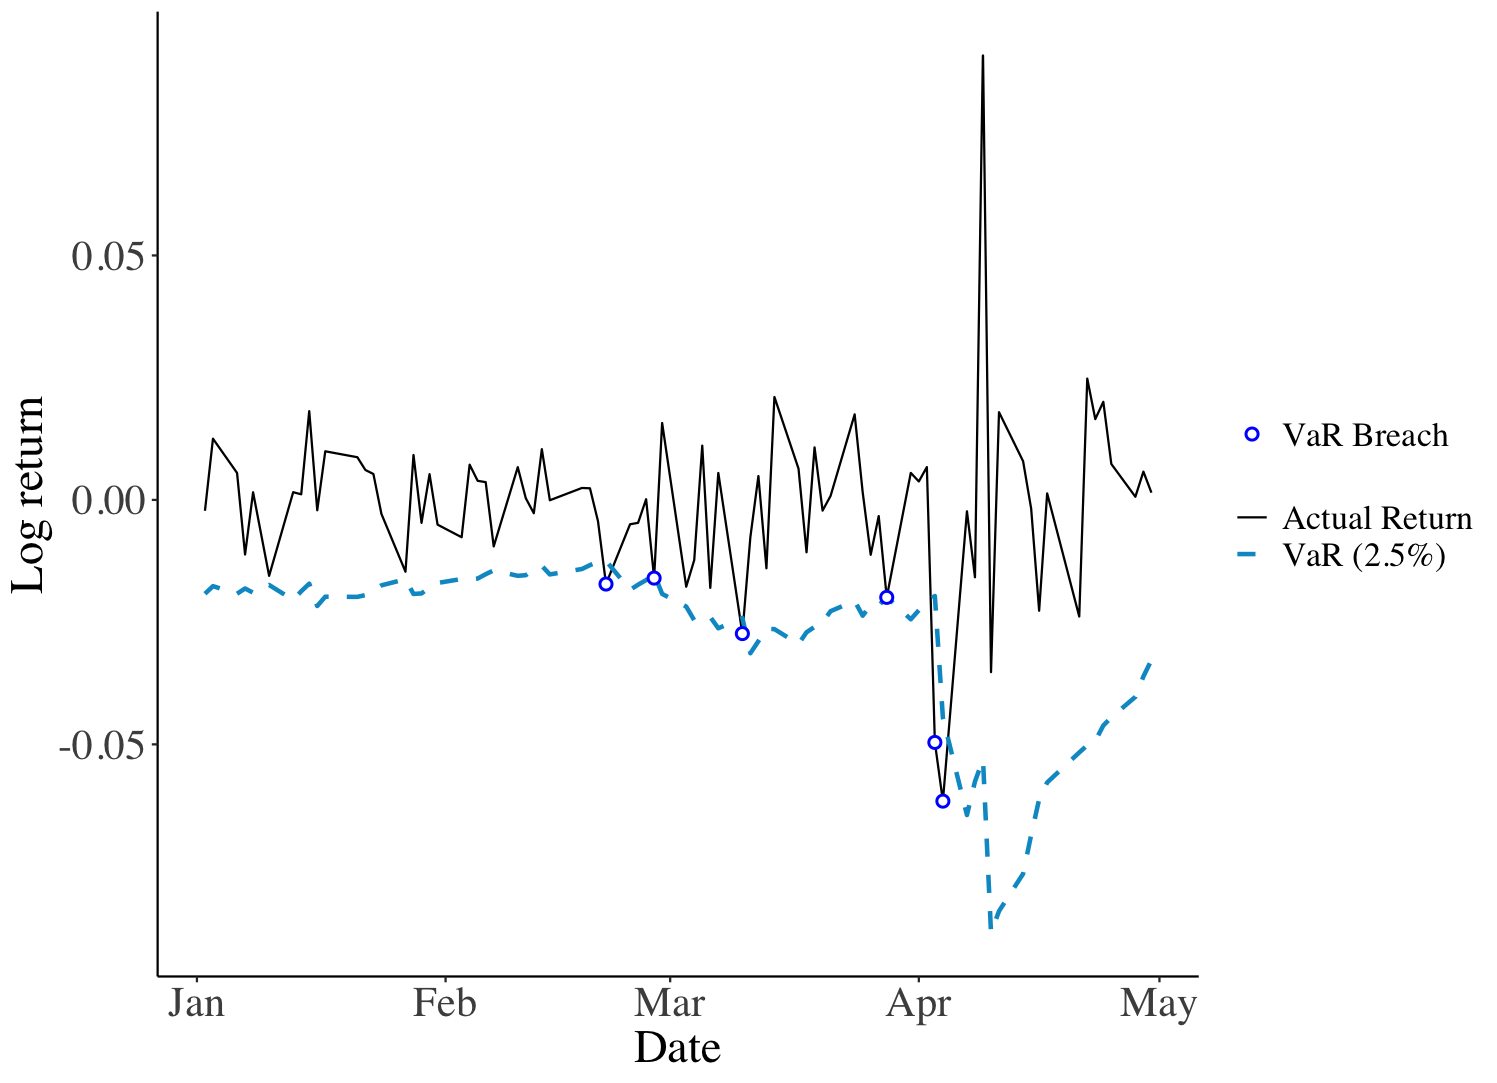
\includegraphics[scale=0.175]{../../plots/4.3.png} % Replace 
   \caption{2.5\% VaR forecast and breaches in the test period, GARCH-Asyt (6 breaches observed; 2 expected).}
    \label{4.3}
\end{figure}

\begin{figure}[H]
    \centering
    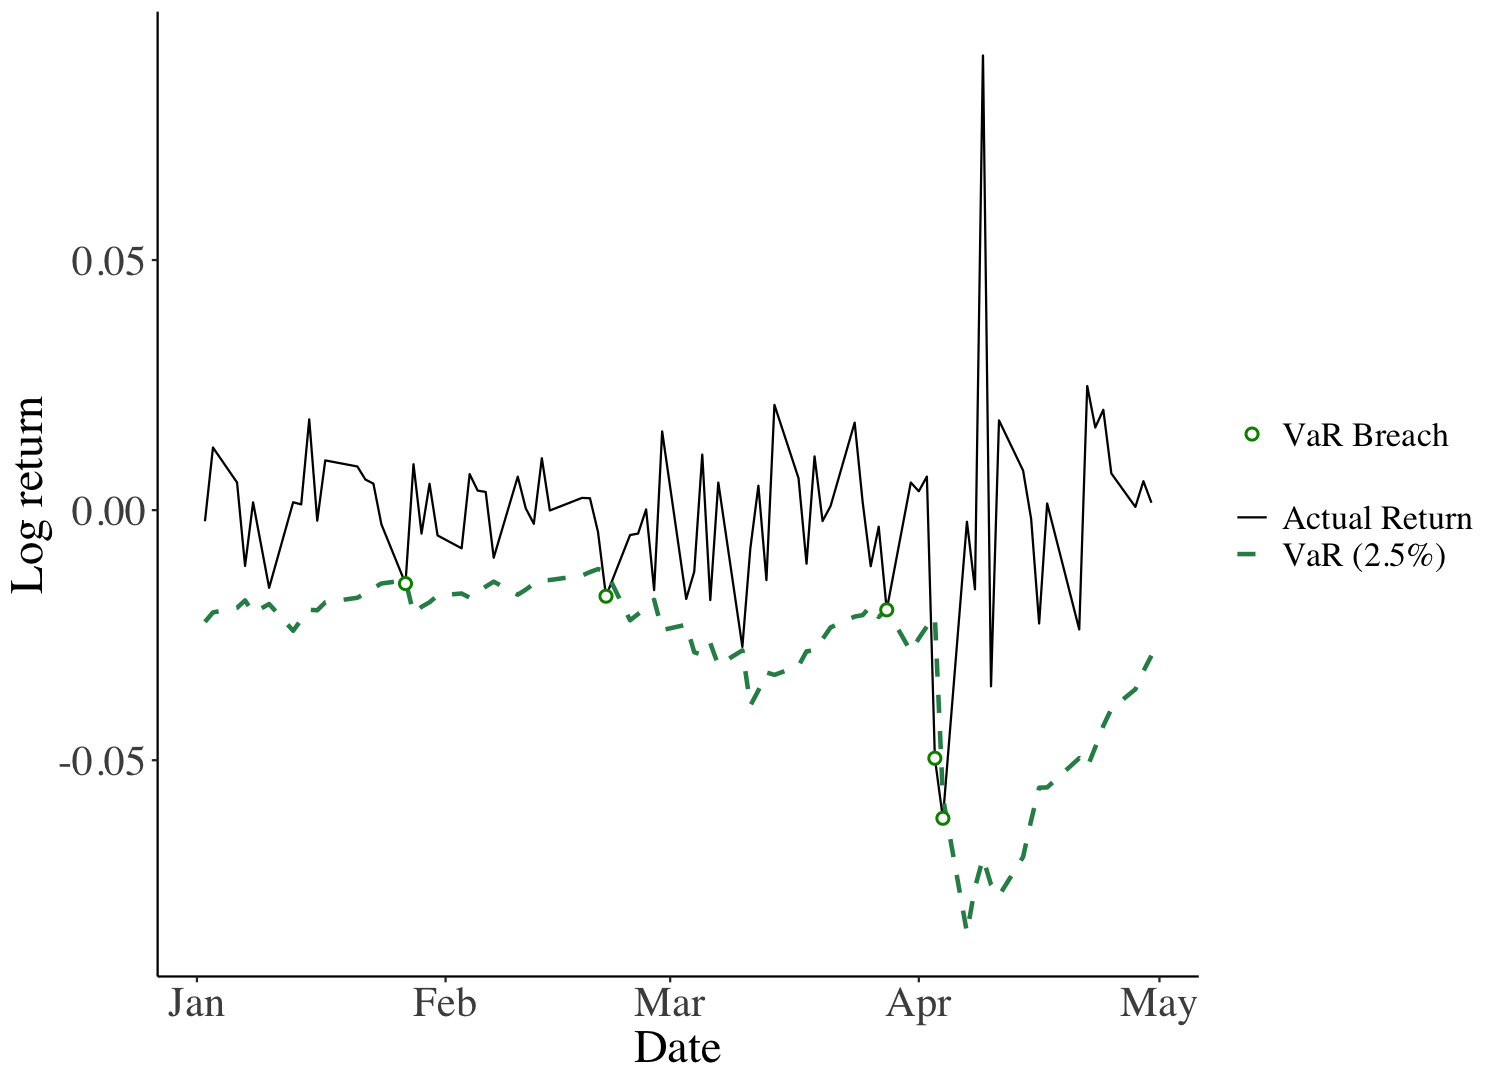
\includegraphics[scale=0.175]{../../plots/4.4.png} % Replace 
   \caption{2.5\% VaR forecast and breaches in the test period, GJR-Asyt (5 breaches observed; 2 expected).}
    \label{4.4}
\end{figure}

To improve the coverage of VaR and account for model risk, sources of uncertainty such as parameter estimation, model specification, and error distribution can be incorporated. \citeA{mazzeu2018uncertainty} propose several approaches to address these issues in ARMA models, which can be extended to the volatility models considered here.

As a simpler alternative, this chapter considers the use of Expected Shortfall (ES) as a way to stress the VaR forecast. Although ES is an expected value and does not correspond to a specific coverage level, it provides a more conservative risk measure by reflecting the average loss in the tail, thus functioning as a stressed version of VaR. Figures 4.5 and 4.6 display the 2.5\% Expected Shortfall for the previous models. It is worth noting that, among the cluster of consecutive breaches in early April in both Figures, only the first one also exceeds the ES forecast, illustrating how ES tempers the speed at which the conservative threshold is itself broken once volatility surges.

\begin{figure}[H]
    \centering
    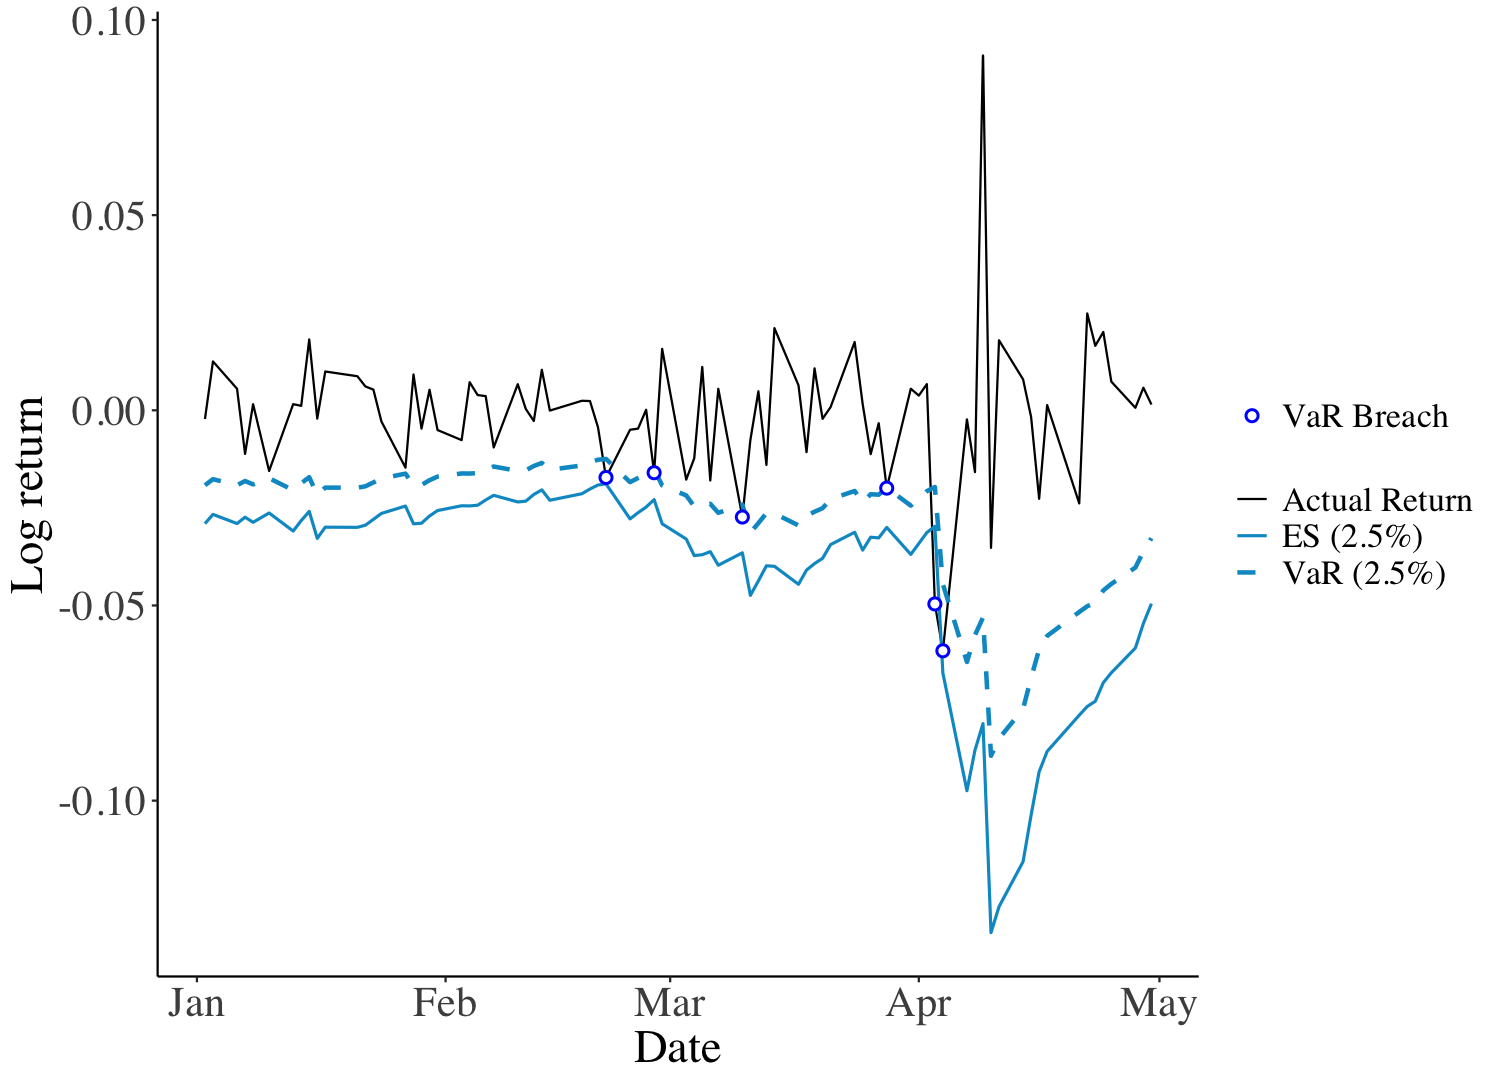
\includegraphics[scale=0.18]{../../plots/4.5.png} % Replace 
   \caption{2.5\% Expected Shortfall forecast in the test period,  GARCH-Asyt.}
    \label{4.5}
\end{figure}

\begin{figure}[H]
    \centering
    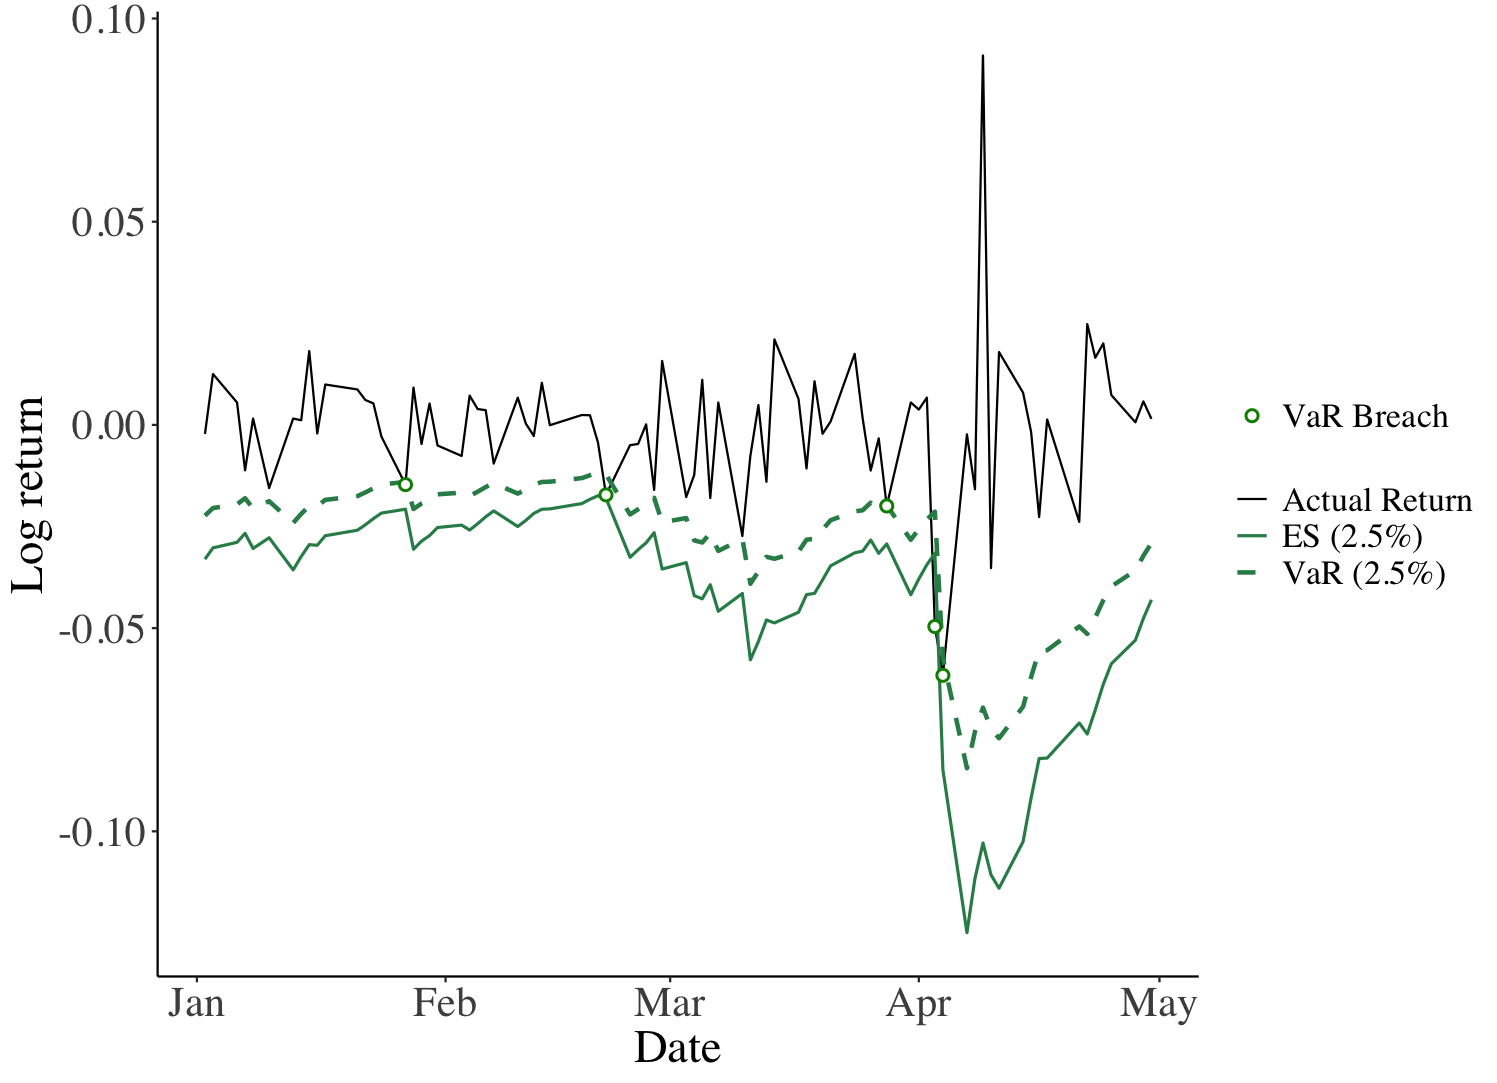
\includegraphics[scale=0.18]{../../plots/4.6.png} % Replace 
   \caption{2.5\% Expected Shortfall forecast in the test period,  GJR-Asyt.}
    \label{4.6}
\end{figure}

\citeA{christoffersen1998evaluating} provides an intuitive framework to evaluate the performance of VaR forecasts by testing two essential properties: coverage and independence.

Recall that a 1-day ahead VaR forecast at level $p$, denoted $\text{VaR}_{t + 1}^p$, implies that the actual return will fall below this threshold only $p \times 100\%$ of the time. Given a time series of ex-ante VaR forecasts and corresponding realized returns, the hit sequence of violations can be defined as follows:
\begin{equation}
I_{t+1} =
\begin{cases}
1, & \text{if } R_{t+1} < -\text{VaR}_{t+1}^p \\
0, & \text{if } R_{t+1} \geq -\text{VaR}_{t+1}^p.
\end{cases}
\label{eq:4.5}
\end{equation}

If the VaR model is correctly specified, violations should occur randomly with probability $p$ each day, implying that the hit sequence $\{I_{t+1}\}$ is independently and identically distributed (i.i.d.) as a $\text{Bernoulli}(p)$ random variable. Predictability of violations based on past information would indicate model misspecification and suggest room for improvement.

Three distinct properties can be tested, beginning with unconditional coverage. This test evaluates whether the observed frequency of breaches matches the expected frequency $p$. Let $\pi$ denote the parameter of the Bernoulli distribution governing the hit sequence, so that $I_{t+1}\sim \text{Bernoulli}(\pi)$. It can be estimated by
$\hat{\pi} = \frac{T_1}{T}$,
where $T_1$ is the number of violations observed in $T$ total observations. Since the Bernoulli likelihood is maximized at the sample mean, $\hat{\pi}=T_1/T$ is the maximum likelihood estimator of $\pi$. The hypotheses are then stated as
\[H_0:\pi=p \quad \text{vs.} \quad H_1:\pi\neq p.\]
The likelihood ratio test statistic for unconditional coverage is given by $LR_{\text{uc}} = -2 \ln\left( \frac{L(p)}{L(\hat{\pi})} \right)$ which, under the null hypothesis, asymptotically follows a $\chi^2$ distribution with 1 degree of freedom.\footnote{This result follows from the general asymptotic theory of likelihood ratio tests: under standard regularity conditions, the likelihood ratio statistic converges in distribution to a chi-squared random variable with degrees of freedom equal to the difference in the number of free parameters under the null and alternative hypotheses. See \citeA{casella2002statistical} for a standard treatment.}

Second, the independence of VaR violations can be assessed. Independence is critical; even if a VaR model achieves correct unconditional coverage, clustered violations would be problematic from a risk management perspective. Ideally, violations should occur randomly and independently, rather than grouping together in time. Therefore, testing for independence involves checking if the violations exhibit temporal clustering.

To conduct this test, assume the hit sequence $\{I_t\}$ follows a first-order Markov process characterized by the transition probability matrix:
\[
\Pi_1 =
\begin{bmatrix}
1 - \pi_{01} & \pi_{01} \\
1 - \pi_{11} & \pi_{11}
\end{bmatrix}.
\]
where, for example, the probability of a VaR violation tomorrow ($I_{t+1}=1$) given no violation today ($I_t=0$) is denoted by $\pi_{01}$. With a sample of $T$ observations, the likelihood function under this first-order Markov assumption is:
\[
L(\Pi_1) = (1 - \pi_{01})^{T_{00}} \, \pi_{01}^{T_{01}} \, (1 - \pi_{11})^{T_{10}} \, \pi_{11}^{T_{11}}.
\]
where $T_{ij}, \ i,j \in \{0,1\}$, is the number of times a state $j$ occurs immediately after state $i$.  The parameters $\pi_{01}$ and $\pi_{11}$ are estimated via maximum likelihood.

The null hypothesis of independence assumes that the probability of a violation does not depend on previous violations, thus simplifying the transition matrix to:
\[
\Pi_0 =
\begin{bmatrix}
1 - \pi & \pi \\
1 - \pi & \pi
\end{bmatrix}.
\]
The likelihood ratio test for independence and its distribution under the null hypothesis is:
\[
LR_{\text{ind}} = -2 \ln \left[ \dfrac{L(\hat{\Pi}_0)}{L(\hat{\Pi}_1)} \right] \dot\sim \chi^2_1,
\]
where $L(\hat{\Pi}_0)$ and $L(\hat{\Pi}_1)$ represent the maximum likelihood under the null hypothesis of independence and under the alternative hypothesis allowing dependence, respectively.

Lastly, it is critical to jointly test conditional coverage, evaluating simultaneously both independence and correct unconditional coverage. This is done via the conditional coverage likelihood ratio test which, under the null hypothesis, asymptotically follows a $\chi^2$ distribution with 2 degrees of freedom:
\[
LR_{\text{cc}} = -2 \ln \left[ \dfrac{L(p)}{L(\hat{\Pi}_1)} \right] \dot\sim \chi^2_2.
\]
which decomposes neatly into two previously described components:  $LR_{\text{cc}}=LR_{\text{uc}}+LR_{\text{ind}}$. 

In practice, backtesting frequently suffers from limited data, resulting in a relatively small number of violations $T_1$, which are crucial for the tests. Thus, relying on asymptotic $\chi^2$ distributions may not always be appropriate. Monte Carlo simulated $p$-values provide a robust alternative in this scenario. \citeA{christoffersen2004backtesting} discuss the implementation of such Monte Carlo-based $p$-values, a method originally proposed by Dufour in a 2000 manuscript that the authors cite and that was later published as \citeA{dufour2006monte}.

To calculate these simulated $p$-values, generate 999 random samples of $\text{i.i.d. Bernoulli}(p)$ variables, each of length $T$, matching the actual sample size. From these artificial samples, compute 999 simulated test statistics, denoted as $\{\widetilde{LR}_{\text{uc}}(i)\}_{i=1}^{999}$. Finally, the simulated $p$-value is calculated as the proportion of simulated $LR_{\text{uc}}$ statistics exceeding the observed test statistic, providing a reliable measure of the test’s significance.

Table~\ref{tab:4.2} reports the theoretical and simulated $p$-values for the tests proposed by \citeA{christoffersen1998evaluating}, applied to the GARCH-Asyt and GJR-Asyt models.

\begin{table}[H]
\centering
\begin{tabular}{llcc}
\toprule
\textbf{Test} & \textbf{p-value} & \textbf{GARCH-Asyt} & \textbf{GJR-Asyt} \\
\midrule
$LR_{\text{uc}}$   & Theoretical & 0.0215 & 0.0735 \\
                   & Simulated   & 0.003 & 0.144 \\
$LR_{\text{ind}}$  & Theoretical & 0.4332 & 0.2793 \\
                   & Simulated   & 0.095 &  0.047 \\
$LR_{\text{cc}}$   & Theoretical & 0.0523 & 0.1123 \\
                   & Simulated   & 0.015 & 0.028 \\
\bottomrule
\end{tabular}
\caption{Theoretical and simulated $p$-values for VaR backtesting statistics.}
\label{tab:4.2}
\end{table}

These models exhibit weak performance: they fail to achieve acceptable coverage, and the violations do not seem independent. As shown in Figures~\ref{4.3} and~\ref{4.4}, two breaches occur in quick succession at the onset of President Trump’s tariff imposition, indicating slow adaptation to a sharp increase in volatility and resulting in clustered VaR violations.

Attention now turns to evaluating the quality of the density forecasts. Focusing on the full forecasted return distribution offers the advantage of potentially increasing the power to reject misspecified risk models.

The GARCH-Asyt and GJR-Asyt models generate a one-step-ahead cumulative distribution forecast for the next day’s return, denoted $F_t(\cdot)$, at the end of each trading day. After observing the actual return $R_{t+1}$, the cumulative probability assigned to this outcome by the forecasted distribution can be evaluated. This probability, known as the Probability Integral Transform (PIT), was introduced by \citeA{diebold1998evaluating} and is defined as:
\begin{equation}
u_{t+1} = F_t(R_{t+1}).
\label{eq:4.6}
\end{equation}

\citeA{diebold1998evaluating} show that if the risk model used to forecast the return distribution is correctly specified, then the sequence $\{u_{t+1}\}$ should be independently and identically distributed as \text{Uniform}(0,1). Intuitively, this means that if the forecasted distribution is correct, the PIT values should not be predictable or systematically biased.

To assess the validity of the risk models considered here, the hypothesis of interest is:

\[H_0: u_{t+1} \sim \text{i.i.d. Uniform}(0,1).\]

\newpage
\citeA{diebold1998evaluating} suggest a visual diagnostic using a histogram of the PIT values $\{u_{t+1}\} $ to assess whether they appear approximately uniform. If systematic deviations from flatness are observed, this may indicate that the forecast distribution is misspecified. Figures~\ref{4.7} and~\ref{4.8} display the PIT histograms for the GARCH-Asyt and GJR-Asyt models over the test period, respectively. There are no evident deviations from uniformity.

\begin{figure}[H]
    \centering
    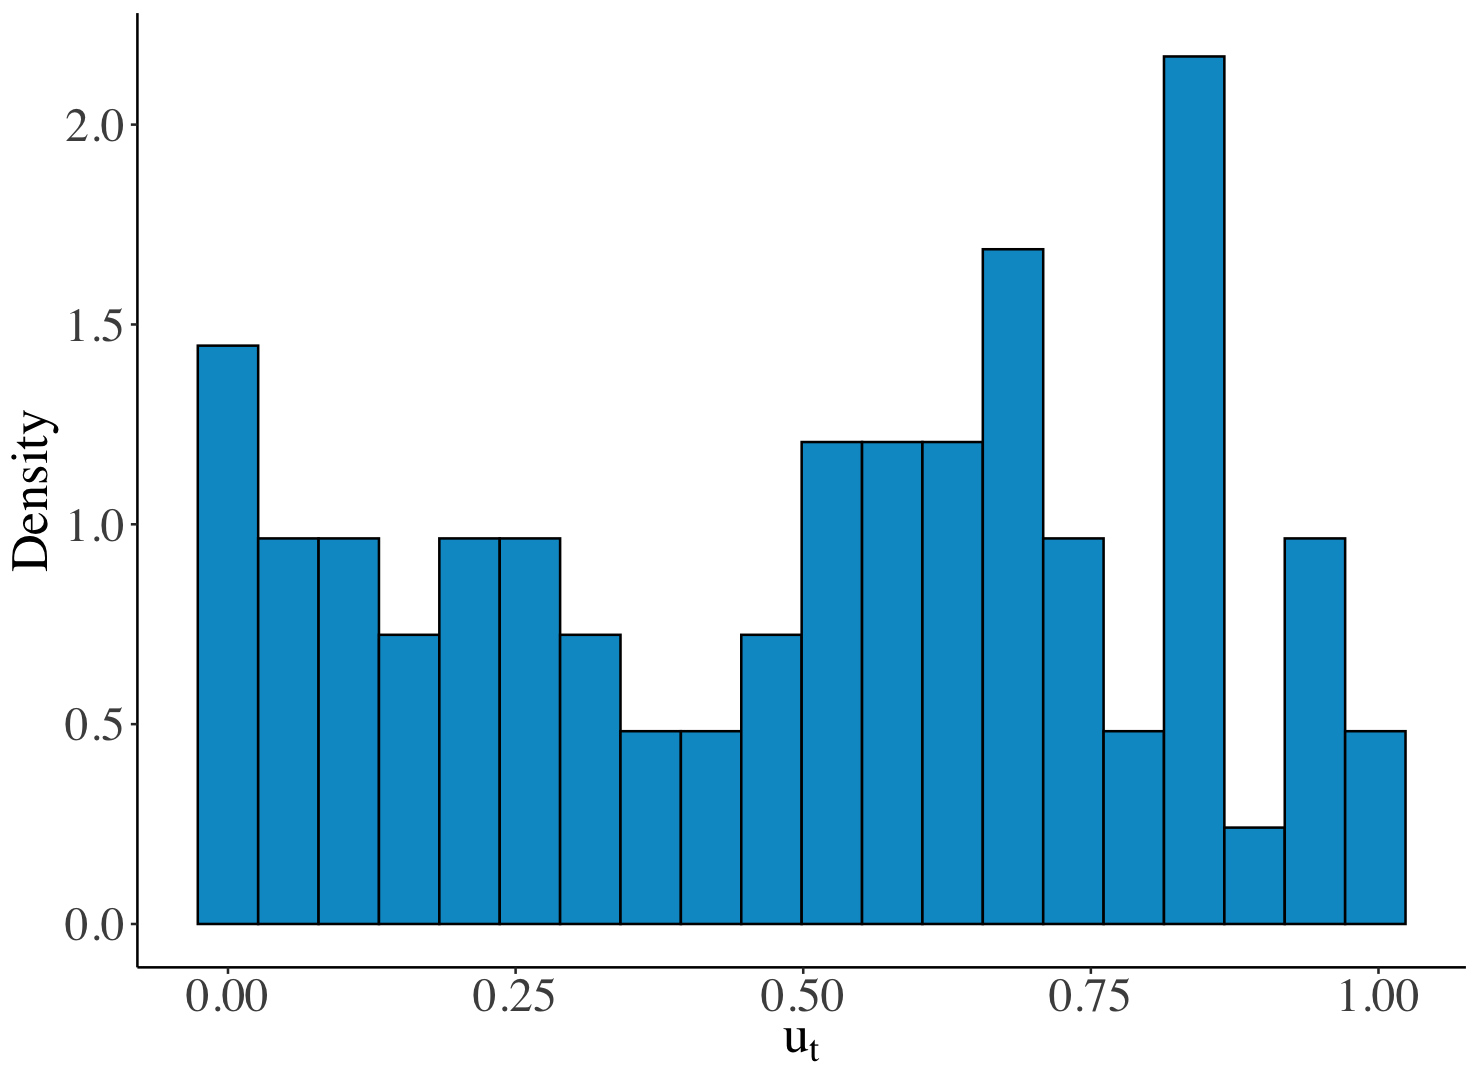
\includegraphics[scale=0.18]{../../plots/4.7.png} % Replace 
   \caption{ Histogram of PIT values, GARCH- Asyt.}
    \label{4.7}
\end{figure}

\begin{figure}[H]
    \centering
    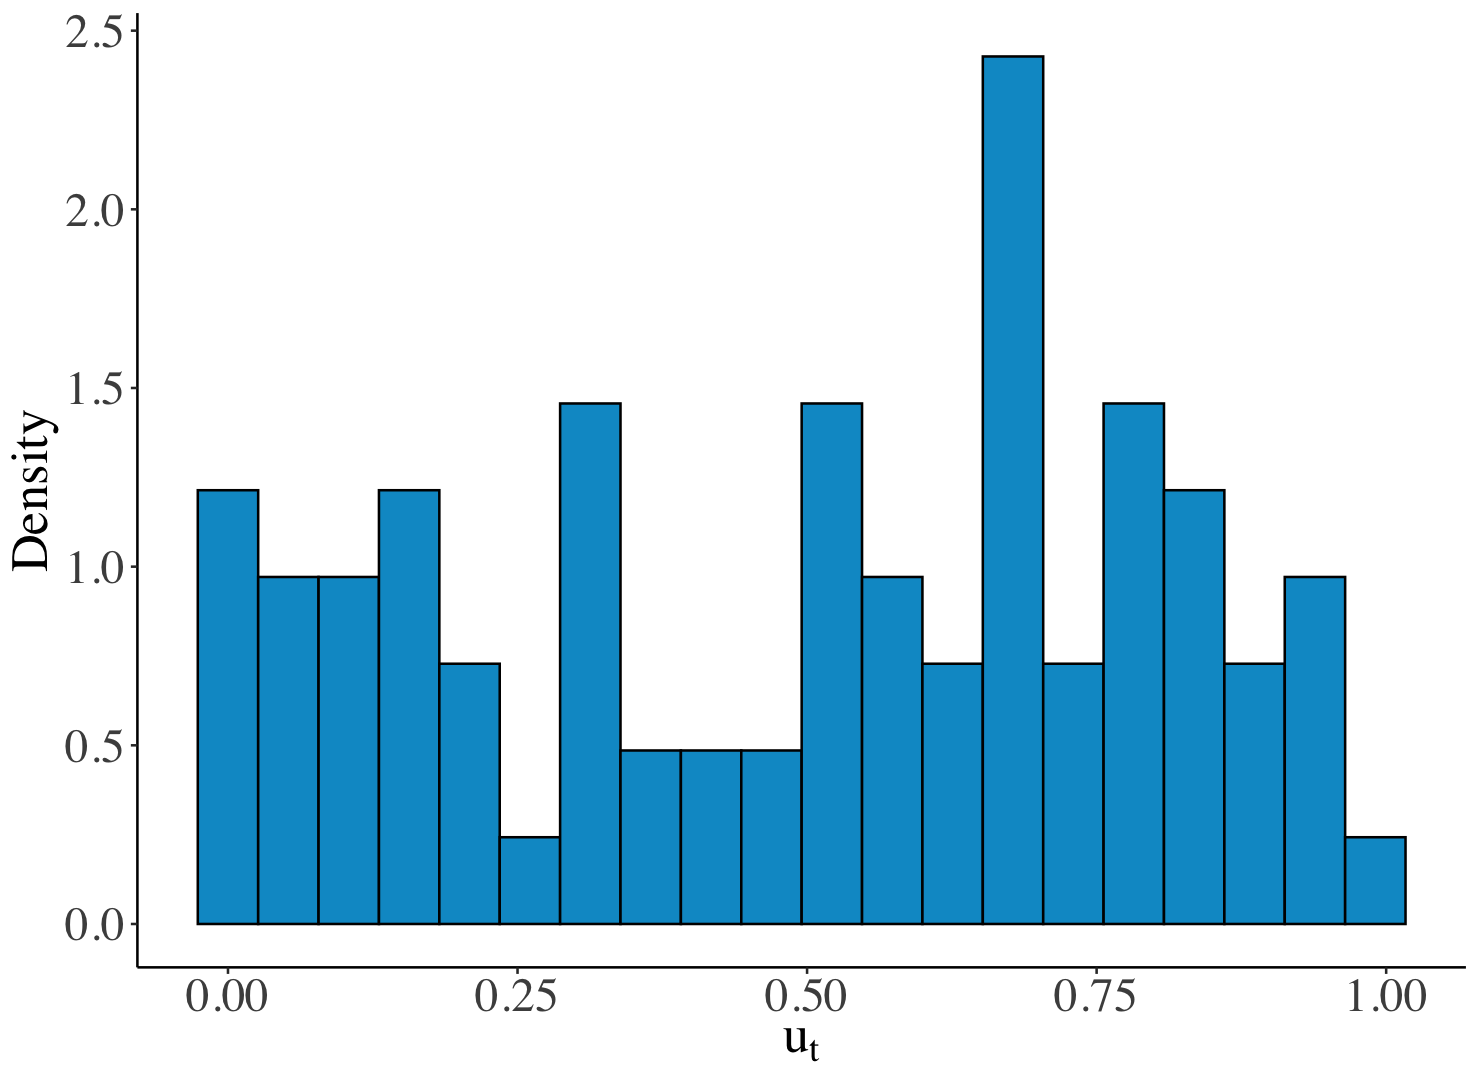
\includegraphics[scale=0.18]{../../plots/4.8.png} % Replace 
   \caption{ Histogram of PIT values, GJR- Asyt.}
    \label{4.8}
\end{figure}

While the histogram provides an intuitive diagnostic, it is not a formal statistical test. As noted by \citeA{Christoffersen2012}, testing the i.i.d. uniformity hypothesis is challenging due to the bounded support of the uniform distribution. To address this, \citeA{berkowitz2001testing} proposes transforming the PIT values to a standard normal scale and applying standard statistical tests to the transformed series:

\begin{equation}
\hat{z}_{t+1} = \Phi^{-1}(u_{t+1}),
\label{eq:4.7}
\end{equation}
where $\Phi^{-1}(\cdot)$ denotes the inverse of the standard normal cumulative distribution function. The hypothesis of interest becomes:

\[H_0: \hat{z}_{t+1} \sim \text{i.i.d. N}(0,1).\]

To test this hypothesis, a Kolmogorov–Smirnov (KS) test can be applied to the GARCH-Asyt and GJR-Asyt models to assess the validity of the density forecasts. Figures~\ref{4.9} and~\ref{4.8} display the empirical cumulative distribution functions of the transformed series $\{\hat{z}_{t+1}\}$ plotted against the standard normal CDF, with the KS test statistics indicated.

\begin{figure}[H]
    \centering
    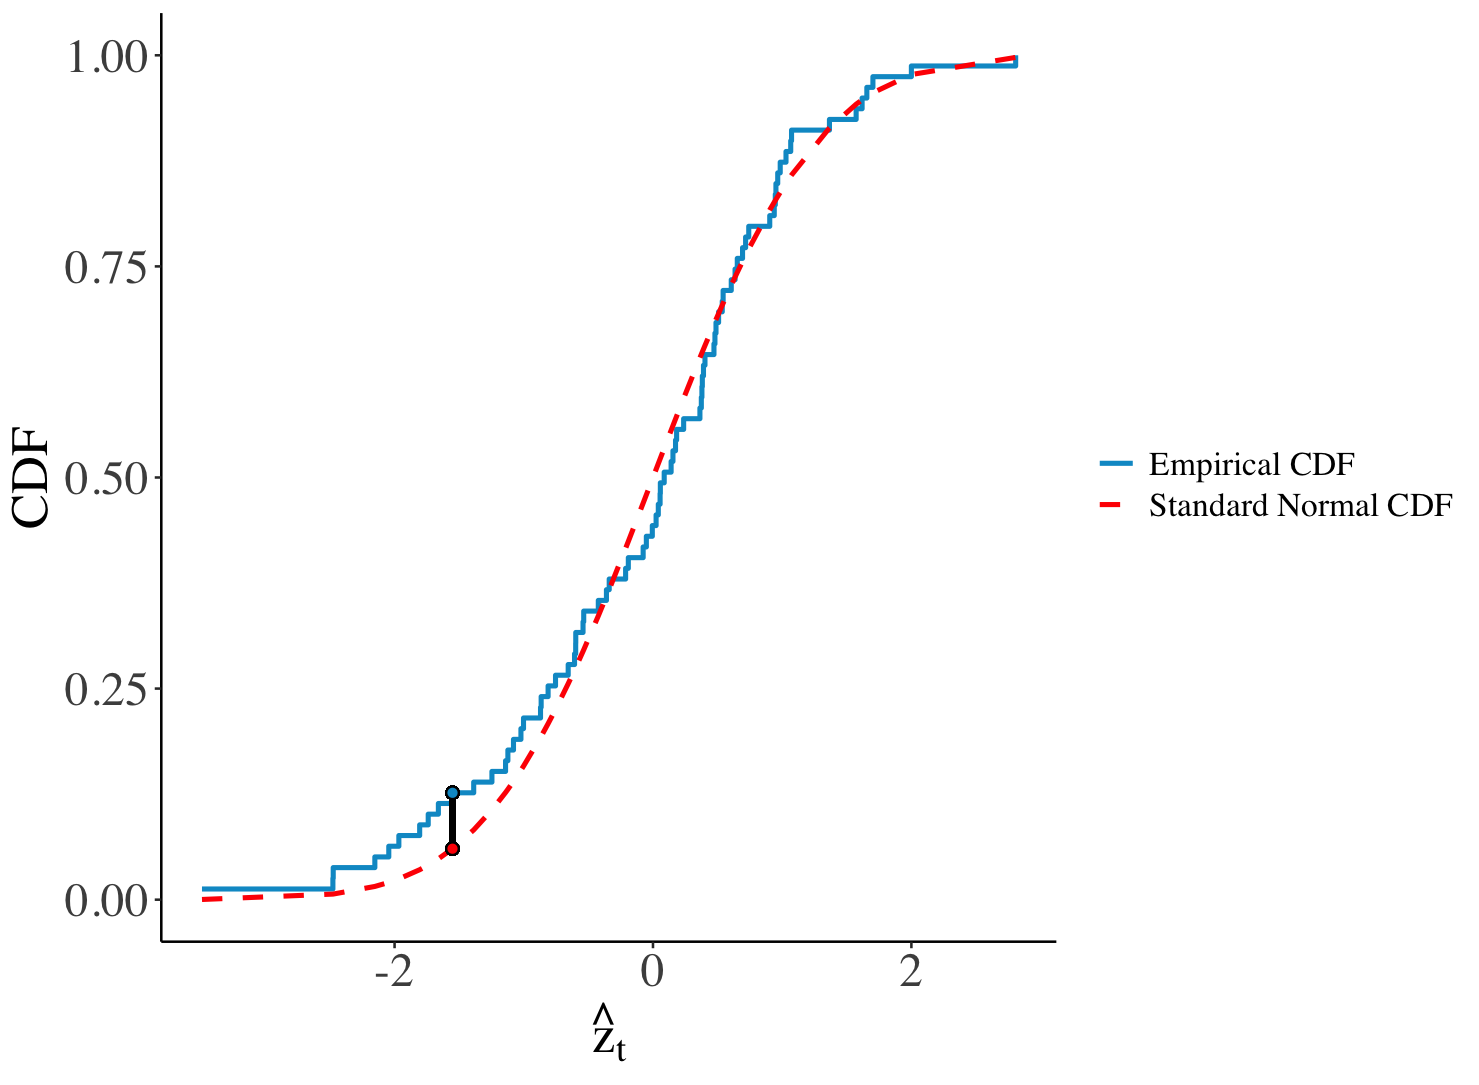
\includegraphics[scale=0.18]{../../plots/4.9.png} % Replace 
   \caption{Kolmogorov-Smirnov test on $\hat{z}_{t+1}$, GARCH-Asyt.}
    \label{4.9}
\end{figure}

\begin{figure}[H]
    \centering
    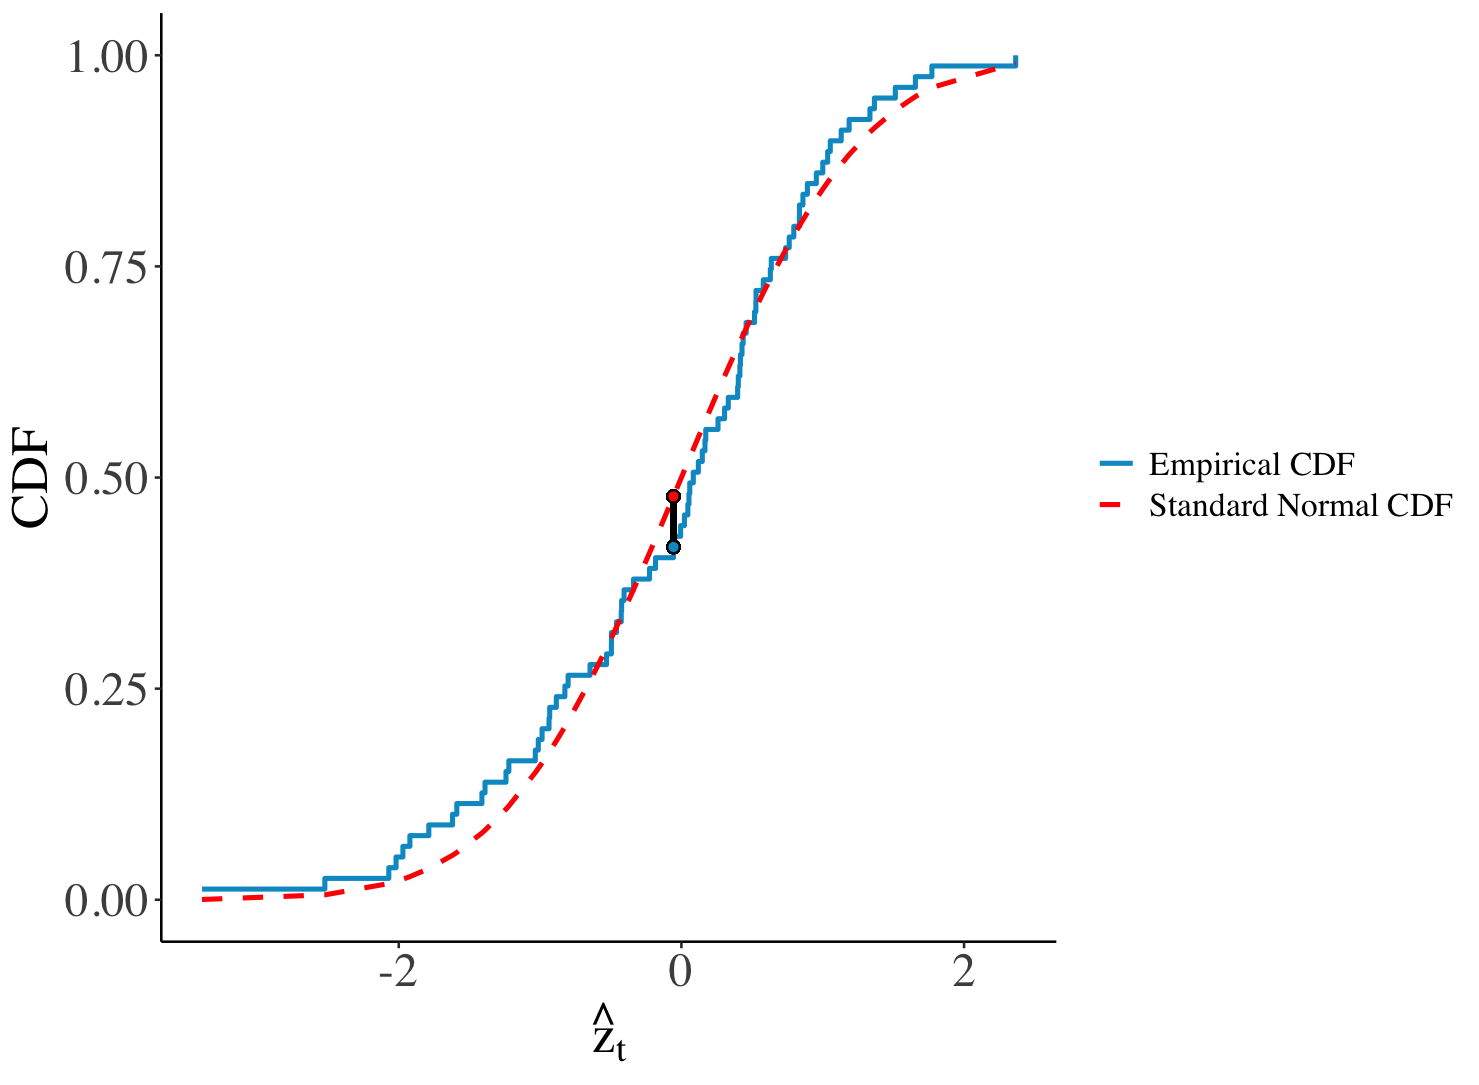
\includegraphics[scale=0.18]{../../plots/4.10.png} % Replace 
   \caption{Kolmogorov-Smirnov test on $\hat{z}_{t+1}$, GJR- Asyt.}
    \label{4.10}
\end{figure}

The resulting $p$-values for the GARCH-Asyt and GJR-Asyt models are 0.8512 and 0.7931, respectively. These values suggest that the hypothesis of normality cannot be rejected, supporting the validity of the models’ density forecasts. In addition, \citeA{berkowitz2001testing} proposes a likelihood ratio (LR) test to jointly assess normality and independence. Specifically, the hypothesis

\[H_0: \hat{z}_{t+1} \sim \text{i.i.d. N}(0,1) \quad vs.\quad H_1: \hat{z}_{t+1} \sim \text{N}(\hat{\mu},\hat{\sigma}^2) \] 

$\text{with autocorrelation }\rho$, can be tested via an LR statistic. The resulting $p$-values for the GARCH-Asyt and GJR-Asyt models are 0.3089 and 0.6577, respectively, indicating that the null hypothesis cannot be rejected.

To formally compare the density forecasts during the test period, the Diebold–Mariano (DM) test introduced by \citeA{diebold1995comparing} is employed. This test compares the accuracy of two competing forecast models under a specified loss function, which in this case is the negative log-likelihood function of the actual returns given the forecasted densities. Using the log-likelihood as a scoring rule follows the suggestion of \citeA{elliott201} for evaluating density forecasts. 

The DM test statistic is defined as:
\[
\text{DM} = \frac{\bar{d}}{\hat{\sigma}_d/\sqrt{T}},\]

where $\bar{d}$ is the average difference in log-likelihood scores, $d_t = \ell^{\text{(GARCH)}}(R_{t+1}|F_{t}) - \ell^{\text{(GJR)}}(R_{t+1}|F_{t})$,

with $\ell^{(m)}(\cdot)$ and $\ell^{(n)}(\cdot)$ representing the log-likelihoods of the two competing models. Here, $\hat{\sigma}_d$ denotes the standard deviation of the series $\{d_t\}$, and $T$ is the sample size. Under the null hypothesis of equal forecast accuracy, the DM statistic follows a standard normal distribution. 

After performing the test, the resulting $p$-value is 0.015, with a positive test statistic, suggesting that the GJR-Asyt density forecast provides significantly better forecasting performance compared to the GARCH-Asyt model. 

\citeA{corradi2006predictive} provide an extensive survey of methods to evaluate and compare density forecasts, both in-sample and out-of-sample. Readers interested in further methods for evaluating density forecasts are referred to this comprehensive survey. 

Attention now turns toward the GARCH-EVT and GJR-EVT models. These models provide conditional tail distributions rather than full-density forecasts. Informally, one might describe them as tail forecasts. Although several frameworks exist to evaluate tail forecasts, such as those proposed by \citeA{berkowitz2001testing} and \citeA{Christoffersen2012}, these approaches cannot be directly adapted to the conditional GARCH-EVT and GJR-EVT models considered here. Thus, these two models will only be assessed from a risk management perspective; a rigorous statistical validation method remains to be formally established. One possible validation strategy could involve adapting the PIT approach specifically for observations exceeding the threshold $u$, but this idea has not yet been fully explored in the reviewed literature.

According to the Pickands–Balkema–de Haan theorem, for sufficiently large threshold $u$,
\[
\frac{F(y) - F(u)}{1 - F(u)} \approx G_{u, \xi,\beta}(y) \quad \text{for } y>u,
\]

where $G_{u, \xi, \beta}(y)$ denotes the cumulative distribution function (CDF) of the generalized Pareto distribution (GPD). Approximating the CDF $F(u)$ of the standardized returns using the empirical distribution, we have:
\[
\hat{F}(u) = \frac{T - N_{u}}{T},
\]
where $N_u$ is the number of threshold exceedances and $T$ is the training sample size. Consequently, the tail distribution can be approximated by:
\[
F(y) \approx  F(u) + G(y)[1 - F(u)] \approx 1 - \frac{N_{u}}{T} \left[ 1 + \frac{\xi(y - u)}{\beta} \right]^{-1/\xi}.
\]
This approximation provides a direct method to estimate quantiles used for VaR calculations. Specifically, for a small tail probability $p$, letting $q = 1 - p$, solving the previous equation for $y$ yields the estimated VaR of the standardized returns:

\begin{equation}
    \text{VaR}_{z,t+1}^{p} =  u - \frac{\beta}{\xi} \left\{ 1 - \left[ \frac{T}{N_{u}} (1 - q) \right]^{-\xi} \right\}.
    \label{eq:4.8}
\end{equation}

Consequently, the VaR of actual returns is given by:
\begin{equation}
    \text{VaR}_{t+1}^{p} =  -\sigma_{t+1}\text{VaR}_{z,t+1}^{p}.
    \label{eq:4.9}
\end{equation}

Following similar logic, the Expected Shortfall (ES) for the GARCH-EVT and GJR-EVT models is defined as:
\begin{equation}
    \text{ES}_{t+1}^{p} =  -\sigma_{t+1}\text{ES}_{z,t+1}^{p},
    \label{eq:4.10}
\end{equation}

where $\text{ES}_{z,t+1}^{p}= \frac{\text{VaR}_{z,t+1}^{p}}{1 - \xi} + \frac{\beta - \xi u}{1 - \xi}.$

Figures~\ref{4.11} and~\ref{4.12} display the forecasted 2.5\% VaR, ES, and the observed VaR breaches during the test period. Notice that these models, which incorporate extreme value theory, yield a more conservative (larger magnitude) VaR and consequently exhibit fewer breaches compared to the asymmetric $t$-distribution models. As with the asymmetric-$t$ models, among the cluster of consecutive breaches in early April only the first one also exceeds the ES forecast, again illustrating how ES tempers the speed at which the conservative threshold is itself broken once volatility surges.

\begin{figure}[H]
    \centering
    \includegraphics[scale=0.17]{../../plots/4.11.png} % Replace 
   \caption{2.5\% VaR, ES, and VaR breaches in the test period, GARCH-EVT (4 breaches observed; 2 expected).}
    \label{4.11}
\end{figure}

\begin{figure}[H]
    \centering
    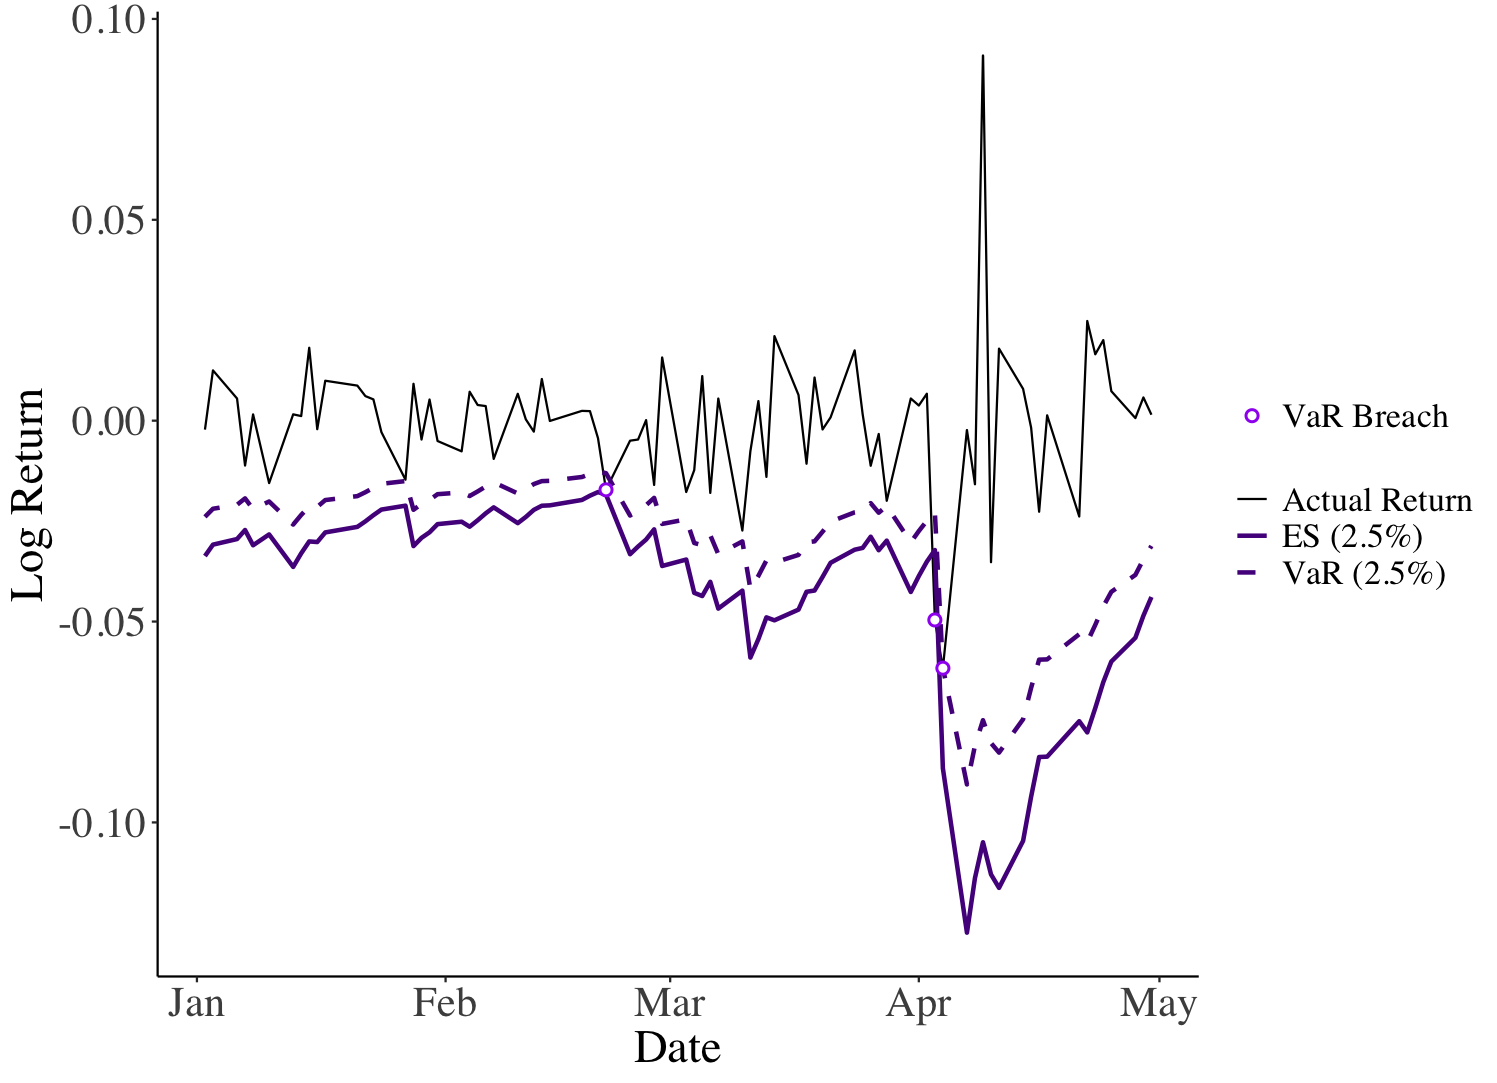
\includegraphics[scale=0.17]{../../plots/4.12.png} % Replace 
   \caption{2.5\% VaR, ES, and VaR breaches in the test period, GJR-EVT (3 breaches observed; 2 expected).}
    \label{4.12}
\end{figure}

The results of the VaR tests using the methodology of \citeA{christoffersen1998evaluating} are summarized in Table~\ref{tab:4.3}.

\begin{table}[H]
\centering
\begin{tabular}{llcc}
\toprule
\textbf{Test} & \textbf{p-value} & \textbf{GARCH-EVT} & \textbf{GJR-EVT} \\
\midrule
$LR_{\text{uc}}$   & Theoretical &  0.2138 &   0.5168 \\
                   & Simulated   & 0.188 & 0.554 \\
$LR_{\text{ind}}$  & Theoretical & 0.1582 & 0.0729 \\
                   & Simulated   & 0.03 & 0.013 \\
$LR_{\text{cc}}$   & Theoretical & 0.1706 & 0.1622 \\
                   & Simulated   & 0.217 & 0.2 \\
\bottomrule
\end{tabular}
\caption{Theoretical and simulated $p$-values for VaR testing statistics.}
\label{tab:4.3}
\end{table}

Both models offer acceptable coverage, but show weaknesses regarding the independence of VaR breaches; primarily due to the two consecutive violations at the onset of the tariff imposed by the United States. This suggests that the models respond slowly to sudden volatility increases. The GJR-EVT model provides acceptable coverage but still fails the independence test. Its comparatively better performance arises from the GJR volatility specification, which adapts more quickly to the volatility increases in the test sample (though not rapidly enough to avoid consecutive breaches), along with the more conservative tail estimation offered by the EVT approach.

Finally, as an exploratory stress-testing exercise, the four models considered (GARCH-Asyt, GJR-Asyt, GARCH-EVT, and GJR-EVT) were evaluated over the 2008 financial crisis to assess their performance from a risk management perspective. The results are presented in Figure~\ref{4.13}, where the dotted lines represent the VaR forecasts under the four models. The EVT-based models exhibit fewer VaR breaches, with the GARCH-EVT model performing best in terms of minimizing violations. Additional stress-testing methodologies and their implementation are discussed by \citeA{Christoffersen2012}.

To complement Figure~\ref{4.13}, Table~\ref{tab:4.4} disaggregates the 2008 VaR breaches into a relatively calmer January--August window and the September--December crisis window.

\begin{table}[H]
\centering
\begin{tabular}{lccc}
\toprule
\textbf{Model} & \textbf{Jan--Aug} & \textbf{Sep--Dec} & \textbf{Total} \\
\midrule
GARCH-Asyt & 9 & 7 & 16 \\
GJR-Asyt   & 8 & 5 & 13 \\
GARCH-EVT  & 4 & 5 & 9  \\
GJR-EVT    & 7 & 5 & 12 \\
\midrule
Expected   & 4.17 & 2.10 & 6.28 \\
\bottomrule
\end{tabular}
\caption{Number of 2.5\% VaR breaches by period and model during the 2008 stress test. The January--August window contains 167 trading days and the September--December window 84; the last row reports the expected number of breaches at the 2.5\% level.}
\label{tab:4.4}
\end{table}

All four specifications exceed their expected number of breaches in both sub-periods, but the deterioration is markedly sharper in September--December. The GARCH-EVT model is essentially well calibrated in the first window (4 observed against 4.17 expected) yet records more than twice the expected breaches in the second (5 against 2.10); the remaining models show an analogous widening of the gap. Since the September--December window contains roughly half as many trading days as the first, the corresponding rise in breach frequency is even more pronounced than the raw counts suggest. This pattern indicates that the four models are unable to adapt quickly enough to the abrupt regime change in September--October 2008.

Up to this point, only univariate models have been considered. While useful, such models may be insufficient for assessing the risk of a portfolio of assets, for which a multivariate framework is required. The next chapter adopts a copula-based approach to model dependence among assets and to produce multivariate forecasts. The main motivation for this choice is that copulas integrate naturally with the univariate models developed so far.

\begin{figure}[H]
    \centering
    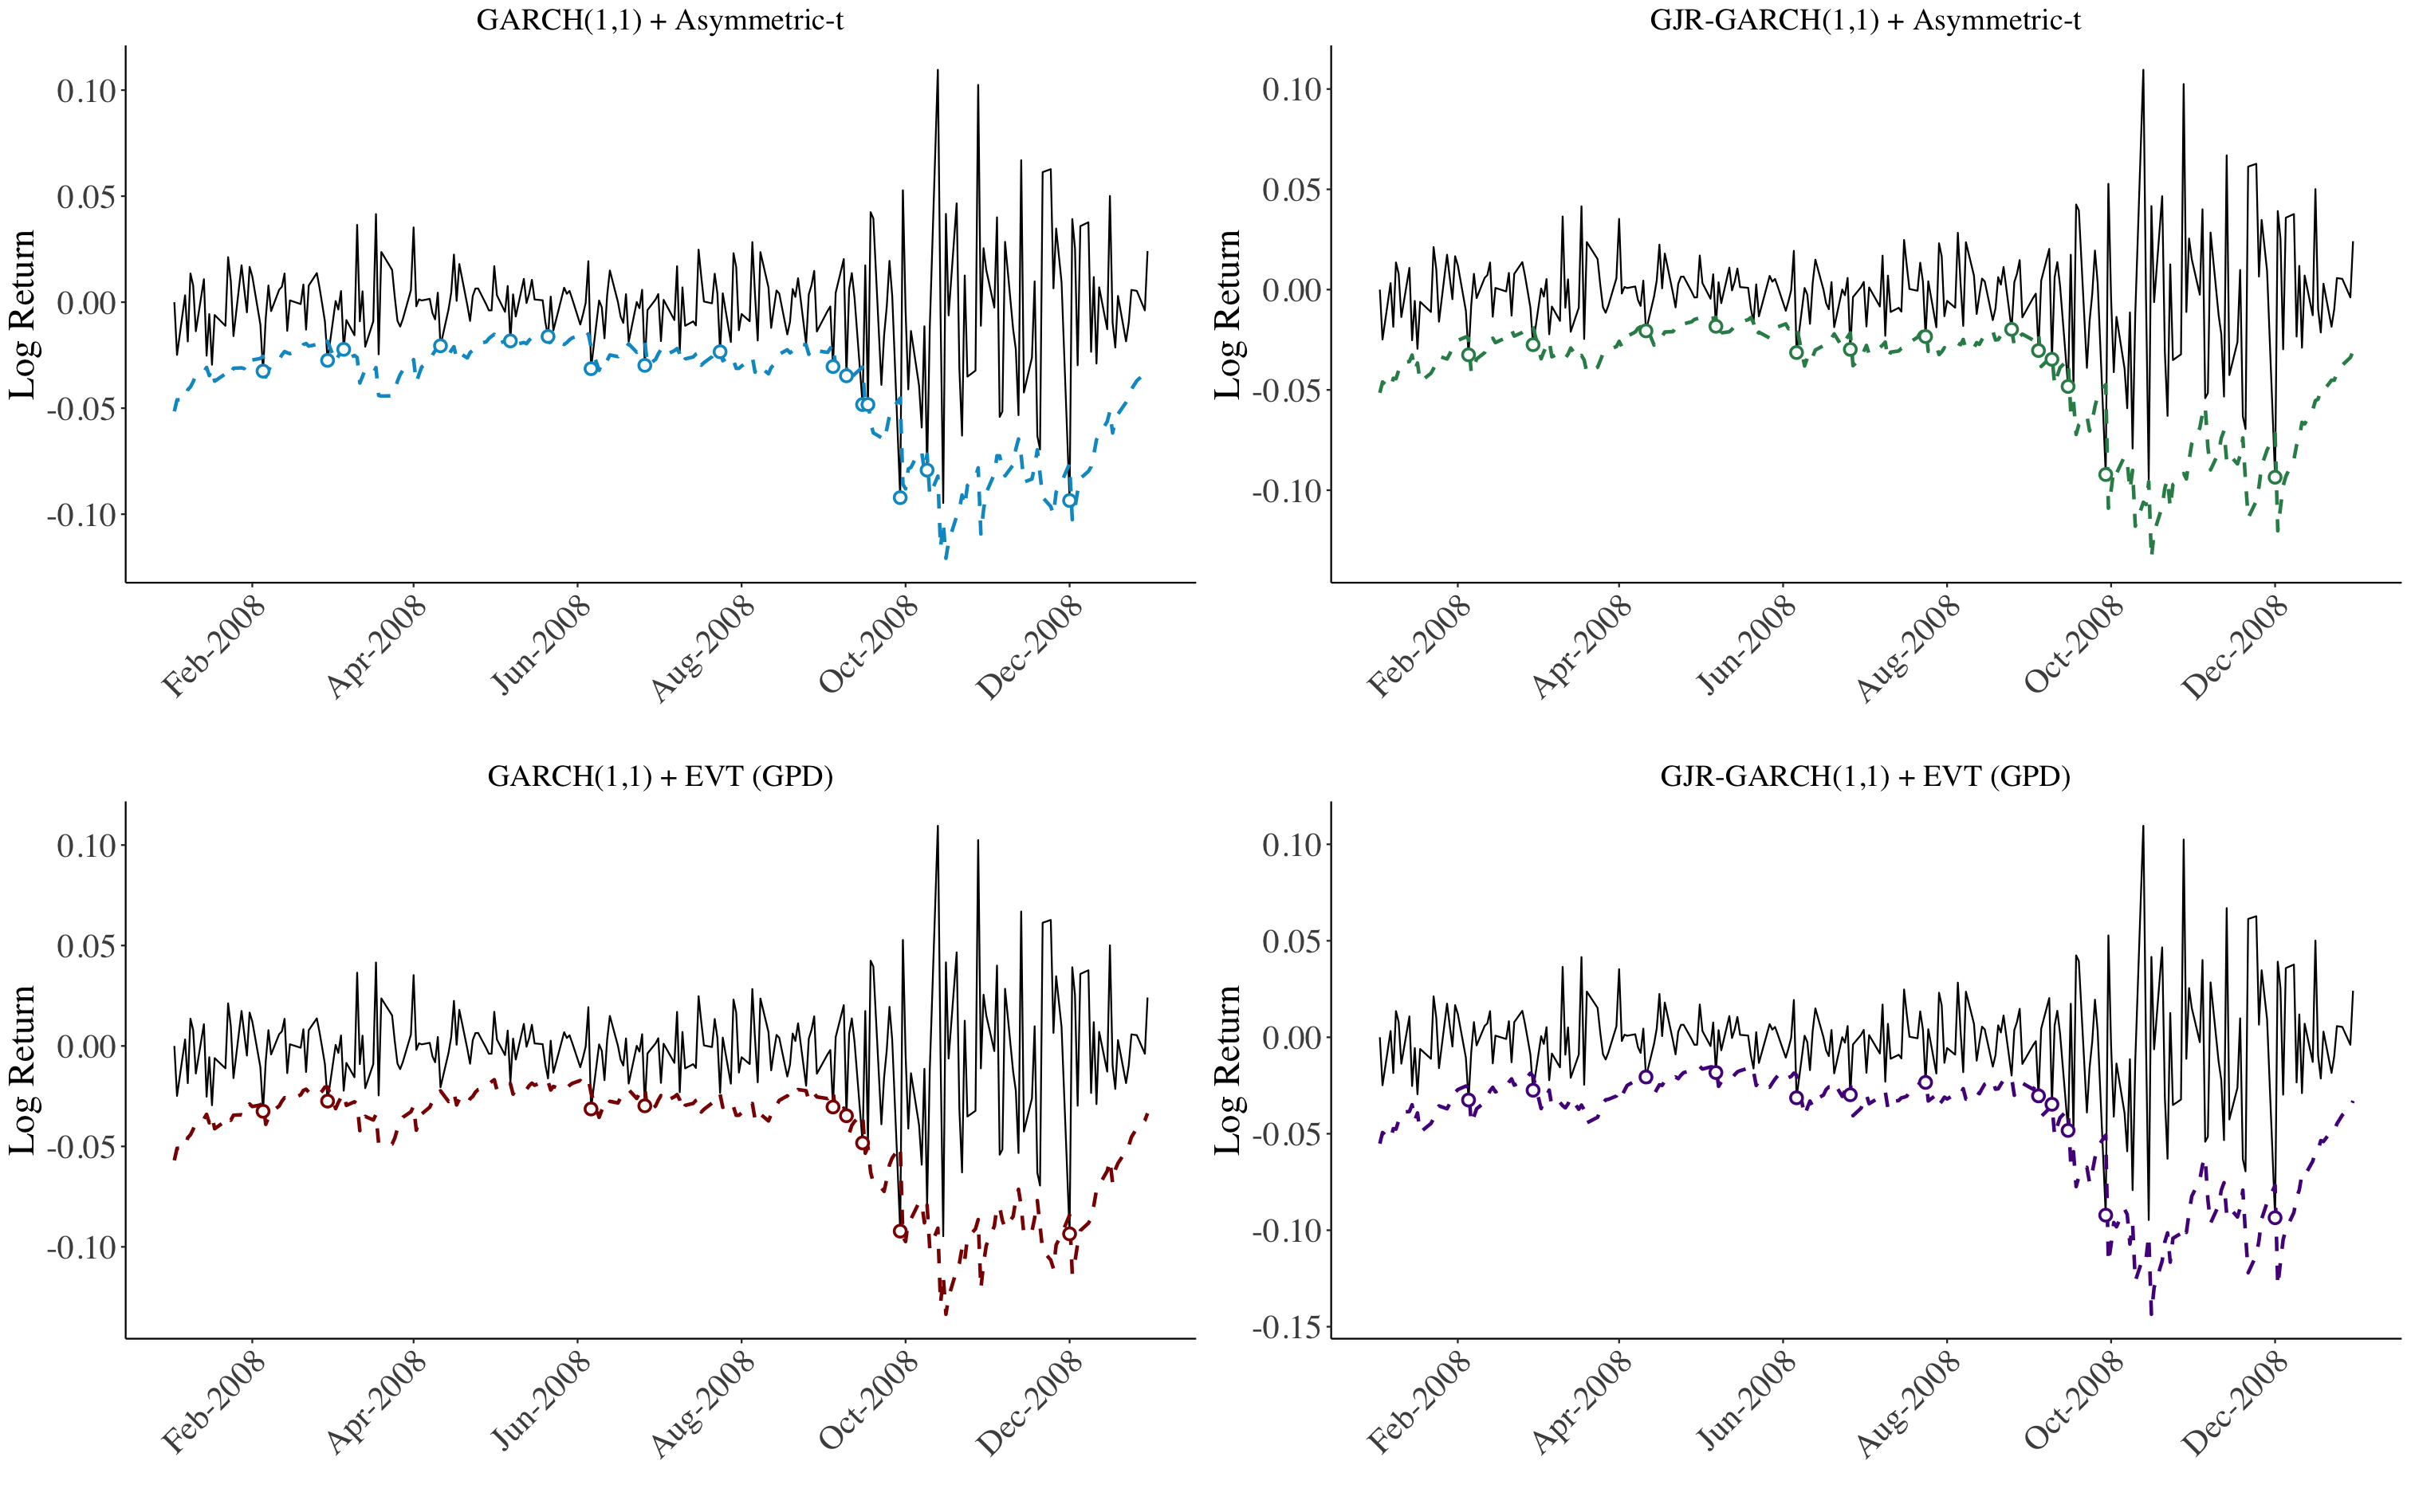
\includegraphics[scale=0.16, angle=90]{../../plots/4.13.png}
    \caption{Stress test of the models.}
    \label{4.13}
\end{figure}

\newpage
\newpage
\chapter{Copula Multivariate Model}
\label{chap:5}

The previous chapters covered various approaches to modeling univariate asset returns. These univariate methods can also be applied directly to portfolio returns. However, while modeling aggregate portfolio returns is suitable for passive risk measurement, it offers limited insight for active risk management. To conduct sensitivity analyses and evaluate diversification benefits, it is necessary to model the dependence structure between individual asset returns. This chapter discusses the copula approach for constructing multivariate risk models.

Alternative approaches to modeling a set of assets (multivariate risk) include those based on the Dynamic Conditional Correlation (DCC) model, which captures the linear dependence between standardized asset returns. A key strength of the DCC approach is its ability to reflect the dynamic correlation patterns introduced in \hyperref[chap:1]{Chapter 1} and illustrated in Figure~\ref{5.1}. Additionally, the DCC model can be combined with multivariate distributions designed to capture asymmetry and heavy tails—features previously discussed in a univariate context but now extended to multiple dimensions. Readers interested in exploring this approach in detail are encouraged to consult \citeA{Christoffersen2012}, which provides a comprehensive overview of the DCC model and compatible multivariate densities.

\begin{figure}[H]
    \centering
    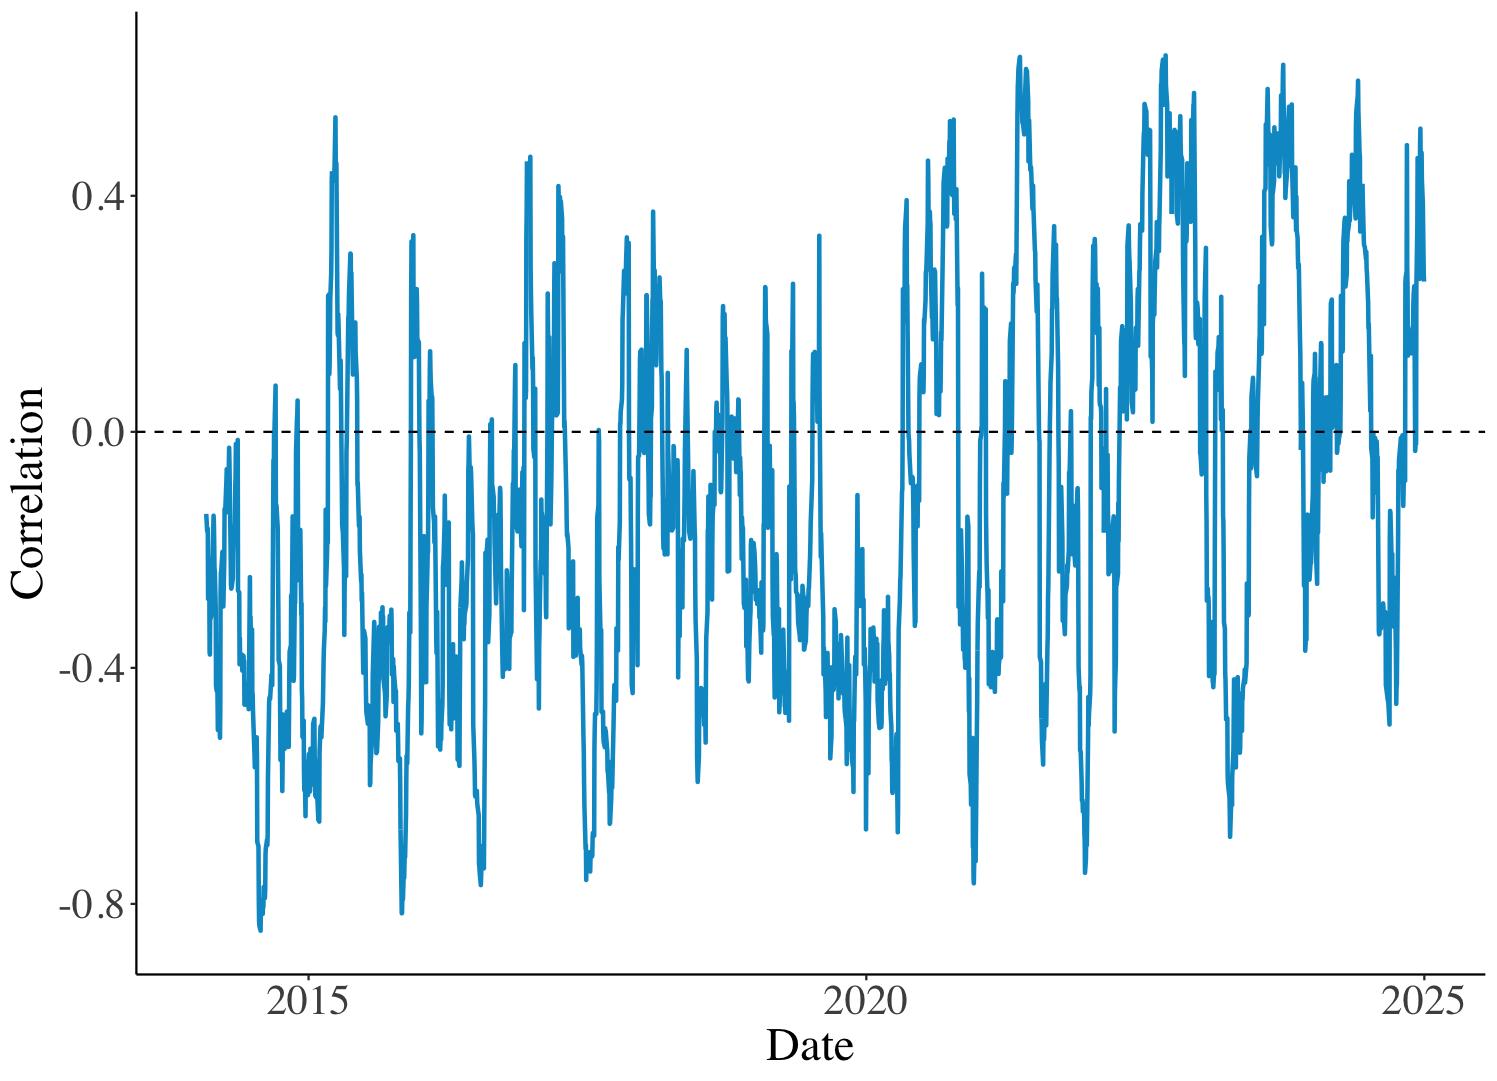
\includegraphics[scale=0.18]{../../plots/5.1.png} % Replace 
   \caption{25-day rolling correlation between the standardized returns of the S\&P 500 and the 10-year Treasury note index (training period).}
    \label{5.1}
\end{figure}

The DCC model approach has two key limitations. First, it focuses exclusively on capturing linear dependencies, thus overlooking more complex nonlinear relationships—particularly in the tails of asset distributions, which are critical for effective risk management. Second, it constrains the univariate models by tying their parameters directly to those estimated within the multivariate framework, potentially limiting their ability to accurately represent individual asset behavior.

The copula modeling approach addresses these issues. It can capture both linear and nonlinear dependencies effectively and allows for separate, flexible univariate models for each asset. These individual univariate models serve as inputs to the copula—analogous to ingredients being blended—resulting in a multivariate model that preserves each asset’s distinctive univariate properties.

Although copula models can be specified dynamically, this chapter employs a static copula for the standardized returns, following \citeA{jondeau2006copulagarch}. In this static specification, the copula parameters are time-invariant (e.g., in a $t$-copula the correlation parameter $\rho^*$ and the degrees of freedom $d$ do not vary with $t$); any dynamics arise solely from the marginal models. Consequently, the specification does not capture time variation in cross-asset dependence (e.g., dynamic correlations). Dynamic copula models have been extensively developed by \citeA{patton2006modelling}, \citeA{patton2011factor}, and \citeA{christoffersen2011joint}. In particular, \citeA{christoffersen2011joint} embed Dynamic Conditional Correlation dynamics within the copula, yielding time-varying dependence.

From a risk management perspective, the tail dependence between assets warrants particular attention. A portfolio containing assets with strongly correlated left-tail returns could suffer significant losses during sharp market downturns. To visualize such tail dependencies, threshold correlations play a key role. The threshold correlation between two standardized returns $z_{1,t}$ and $z_{2,t}$ at level $p$ is defined as
\begin{equation}
\rho(r_{1,t}, r_{2,t}; p) =
\begin{cases}
\text{Corr}\left(z_{1,t}, z_{2,t} \mid z_{1,t} \leq z_1(p) \text{ and } z_{2,t} \leq z_2(p)\right), & \text{if } p \leq 0.5 \\[0.5em]
\text{Corr}\left(z_{1,t}, r_{2,t} \mid z_{1,t} > z_1(p) \text{ and } z_{2,t} > z_2(p)\right), & \text{if } p > 0.5
\end{cases}
\label{eq:5.1}
\end{equation}


where $z_{i}(p)$ represents the $p$-th percentile of the standardized returns of asset $i$.

In other words, the threshold correlation measures the correlation between two assets conditioned on both returns being simultaneously below their respective $p$-th percentiles (for $p<0.5$) or above these percentiles (for $p>0.5$). Calculating threshold correlations across a range of $p$-values and plotting these correlations yields the threshold correlation plot. As noted by \citeA{Christoffersen2012}, threshold correlations reveal how asset returns behave jointly during extreme events—large negative or positive returns—thus providing insights into the shape of the tails of their joint distribution.

Figure~\ref{5.2} displays the threshold correlation plot between the S\&P 500 returns and the 10-year Treasury bond returns standardized by their respective GARCH(1,1) volatilities. For values of $p$ close to 0 or 1, the number of observations becomes limited, which prevents reliable correlation estimation; thus, only correlations computed with at least 25 observations are presented. Although the extreme correlations exhibit considerable variability and should be interpreted cautiously, an important pattern emerges clearly: correlations increase as returns move deeper into the tails. This indicates a heavy-tailed bivariate distribution between stock and bond returns. Additionally, note that there is asymmetry in the tail dependence, the right tail exhibits a higher correlation.

\begin{figure}[H]
    \centering
    \includegraphics[scale=0.43]{../../plots/5.2.png} % Replace 
   \caption{Threshold correlation of GARCH(1,1) standardized returns (training period).}
    \label{5.2}
\end{figure}

Such tail dependence exemplifies the nonlinear relationships that the copula modeling approach aims to capture and replicate. The results in Figure~\ref{5.2} underscore the importance of modeling nonlinear left-tail dependencies between stocks and bonds. An influential application of threshold correlations is provided by \citeA{okimoto2008asymmetric}, who investigates asymmetric dependence structures among international equity markets.

Following the exposition by \citeA{Christoffersen2012}, the theoretical foundation for copula models is provided by Sklar’s theorem. Consider $n$ assets and their respective standardized returns $z_i$, each with potentially distinct marginal probability density functions (PDFs) $f_i(z_i)$ and cumulative distribution functions (CDFs) $u_i=F_i(z_i)$ for $i = 1, 2, \ldots, n$. Sklar’s theorem states that for a very general class of multivariate cumulative distribution functions $ F(z_1, \ldots, z_n)$ with marginals $ F_1(z_1), \ldots, F_n(z_n)$, there exists a unique copula function $G(\cdot)$ that links these marginals to form the joint distribution:
\[
F(z_1, \dots, z_n) = G(F_1(z_1), \dots, F_n(z_n)) = G(u_1, \dots, u_n).
\]
The function $G(u_1, \dots, u_n)$ is referred to as the copula CDF. In line with Sklar’s theorem, the corresponding multivariate probability density function (PDF) can be expressed as:
\[
\begin{aligned}
f(z_1, \dots, z_n) &= \frac{\partial^n G(F_1(z_1), \dots, F_n(z_n))}{\partial z_1 \cdots \partial z_n} \\
&= \frac{\partial^n G(u_1, \dots, u_n)}{\partial u_1 \cdots \partial u_n} \times \prod_{i=1}^n f_i(z_i) \\
&= g(u_1, \dots, u_n) \times \prod_{i=1}^n f_i(z_i),
\end{aligned}
\]
where the copula PDF $g(u_1, \dots, u_n)$ is defined by:
\[
g(u_1, \dots, u_n) \equiv \frac{\partial^n G(u_1, \dots, u_n)}{\partial u_1 \cdots \partial u_n}.
\]
Taking logarithms simplifies the representation as follows:
\[
\ln f(z_1, \dots, z_n) = \ln g(u_1, \dots, u_n) + \sum_{i=1}^n \ln f_i(z_i).
\]

This decomposition demonstrates that constructing a complex multivariate density can be performed in two steps. First, individual marginal distributions $f_1(z_1), \ldots, f_n(z_n)$ are estimated independently using methods outlined in previous chapters. Second, the copula density function g$(u_1, \ldots, u_n)$ is chosen and estimated using the marginal probability values $u_i$ as input data.
\newpage
An important practical advantage of this method is that it simplifies parameter estimation: the parameters of the marginal distributions are estimated independently first, reducing the copula estimation to a separate, simpler second step. This property makes high-dimensional modeling feasible and efficient.

While Sklar’s theorem is quite general, holding true for a broad class of multivariate distributions, it does not specify a functional form for $G(u_1, \ldots, u_n)$. Therefore, an appropriate copula model must be selected based on the application and underlying data.

The $t$-copula, widely used in the literature (see, for instance, \citeA{christoffersen2011joint}),can be extended naturally to $n$ assets and, as will be demonstrated subsequently, is capable of reproducing reasonably the threshold correlations shown in Figure~\ref{5.2}. For these reasons, the $t$-copula is selected for our analysis. However, it is important to highlight that \citeA{okimoto2008asymmetric} finds evidence of significant asymmetric dependence structures in financial data, which symmetric copulas—such as Gaussian and $t$-copulas—may fail to fully capture.

The cumulative distribution function of the bivariate $t$-copula is defined as:
\begin{equation}
G(u_1, u_2; \rho^*, d) = t_{(d, \rho^*)} \left( t^{-1}(u_1; d), \, t^{-1}(u_2; d) \right)
\label{eq:5.2}
\end{equation}
where $t_{(d,\rho^*)}(\cdot)$ denotes the (non-standardized) symmetric multivariate $t$-distribution, $t^{-1}(u; d)$ is the inverse CDF of the (non-standardized) symmetric univariate $t$-distribution, and $\rho^*$ is the correlation parameter between $t^{-1}(u_1; d)$ and $t^{-1}(u_2; d)$, commonly known as the copula correlation.

The corresponding probability density function or the bivariate $t$-copula is:
\begin{equation}
\begin{aligned}
g(u_1, u_2; \rho^*, d) &= \frac{
    t_{(d, \rho^*)}(t^{-1}(u_1; d), \, t^{-1}(u_2; d))
}{
    f_{t(d)}(t^{-1}(u_1; d); d) \, f_{t(d)}(t^{-1}(u_2; d); d)
} \\
&= \frac{
    \Gamma\left(\frac{d+2}{2}\right)
}{
    \sqrt{1 - (\rho^*)^2} \, \Gamma\left(\frac{d}{2}\right)
}
\left(
\frac{\Gamma\left(\frac{d}{2}\right)}{\Gamma\left(\frac{d+1}{2}\right)}
\right)^2 \\
&\quad \times
\frac{\left(
1 + \frac{(t^{-1}(u_1; d))^2 + (t^{-1}(u_2; d))^2 - 2\rho^* \, t^{-1}(u_1; d)t^{-1}(u_2; d)}
{d(1 - (\rho^*)^2)}
\right)^{-\frac{d+2}{2}}}
{
\left(
1 + \frac{(t^{-1}(u_1; d))^2}{d}
\right)^{\frac{d+1}{2}}
\left(
1 + \frac{(t^{-1}(u_2; d))^2}{d}
\right)^{\frac{d+1}{2}}},
\end{aligned}
\label{eq:5.3}
\end{equation}
where $f_{t(d)}(\cdot; d)$ denotes the PDF of the symmetric univariate $t$-distribution with $d$ degrees of freedom.

The $t$-copula will be fitted to the standardized returns of two assets: the S\&P 500 and the 10-year Treasury note index (Bloomberg ticker: SPBDU1BT Index). The estimation period spans January 2014 to December 2024, matching the training period used previously for the S\&P 500 returns. Initially, univariate models are fitted separately to each asset following the framework outlined in earlier chapters, namely, a volatility model combined with a density model for the standardized asset returns. Because the copula approach requires complete density forecasts as inputs, only the asymmetric $t$-distribution—among the models discussed in \hyperref[chap:3]{Chapter 3}—is considered here. Table~\ref{tab:5.1} presents the estimated parameters of the GARCH-Asyt and GJR-Asyt models applied to the Treasury note index, following the specification given in Equations~\eqref{eq:3.2}, \eqref{eq:3.3}, and \eqref{eq:3.4}.

\begin{table}[H]
\footnotesize
\centering
\begin{tabular}{lcccccc}
\toprule
\textbf{Model} & $\omega$ & $\alpha$ & $\beta$ & $\theta$ & $d_1$ & $d_2$ \\
\midrule
GARCH-Asyt &  $3.46 \mathrm{e}{-7}$ & 0.007 & 0.92 & - & 11.01 & $7.5 \mathrm{e}{-3}$ \\
GJR-Asyt & $3.97\mathrm{e}{-7}$ & 0.007 &  0.91 & 0.0344 &  10.97 &  0.0021 \\
\bottomrule
\end{tabular}
\caption{Bond index estimated parameters.}
\label{tab:5.1}
\end{table}
For each asset, two sets of standardized returns are obtained based on the GARCH(1,1) and GJR(1,1) specifications. This yields four potential copula model combinations. To simplify the analysis, only two cases are considered: i) both assets follow the GARCH-Asyt model, and ii) both follow the GJR-Asyt model. Table~\ref{tab:5.2} reports the fitted copula parameters of the GARCH-GARCH and GJR-GJR models. 
\begin{table}[H]
\footnotesize
\centering
\begin{tabular}{lcc}
\toprule
\textbf{Copula model} & $\rho^*$ & $d$ \\
\midrule
GARCH-GARCH &  $-0.2121$ & 4.9671  \\
GJR-GJR & $-0.2088$ & 4.8304  \\
\bottomrule
\end{tabular}
\caption{Copula models estimated parameters.}
\label{tab:5.2}
\end{table}
Using the estimated copula model, it is possible to simulate data and examine whether the model-implied threshold correlations match the empirical pattern observed in Figure \ref{5.2}. Figures~\ref{5.3} and \ref{5.4} display the simulated threshold correlations obtained from the GARCH-GARCH and GJR-GJR copula models, respectively, alongside the empirical threshold correlations derived from the standardized returns. The $t$-copula successfully reasonably replicates the increasing correlation observed in the tails. However, it is worth mentioning that the standardized returns exhibit slightly higher correlation in the right tail, a subtle feature the symmetric $t$-copula cannot fully replicate.
\begin{figure}[H]
    \centering
    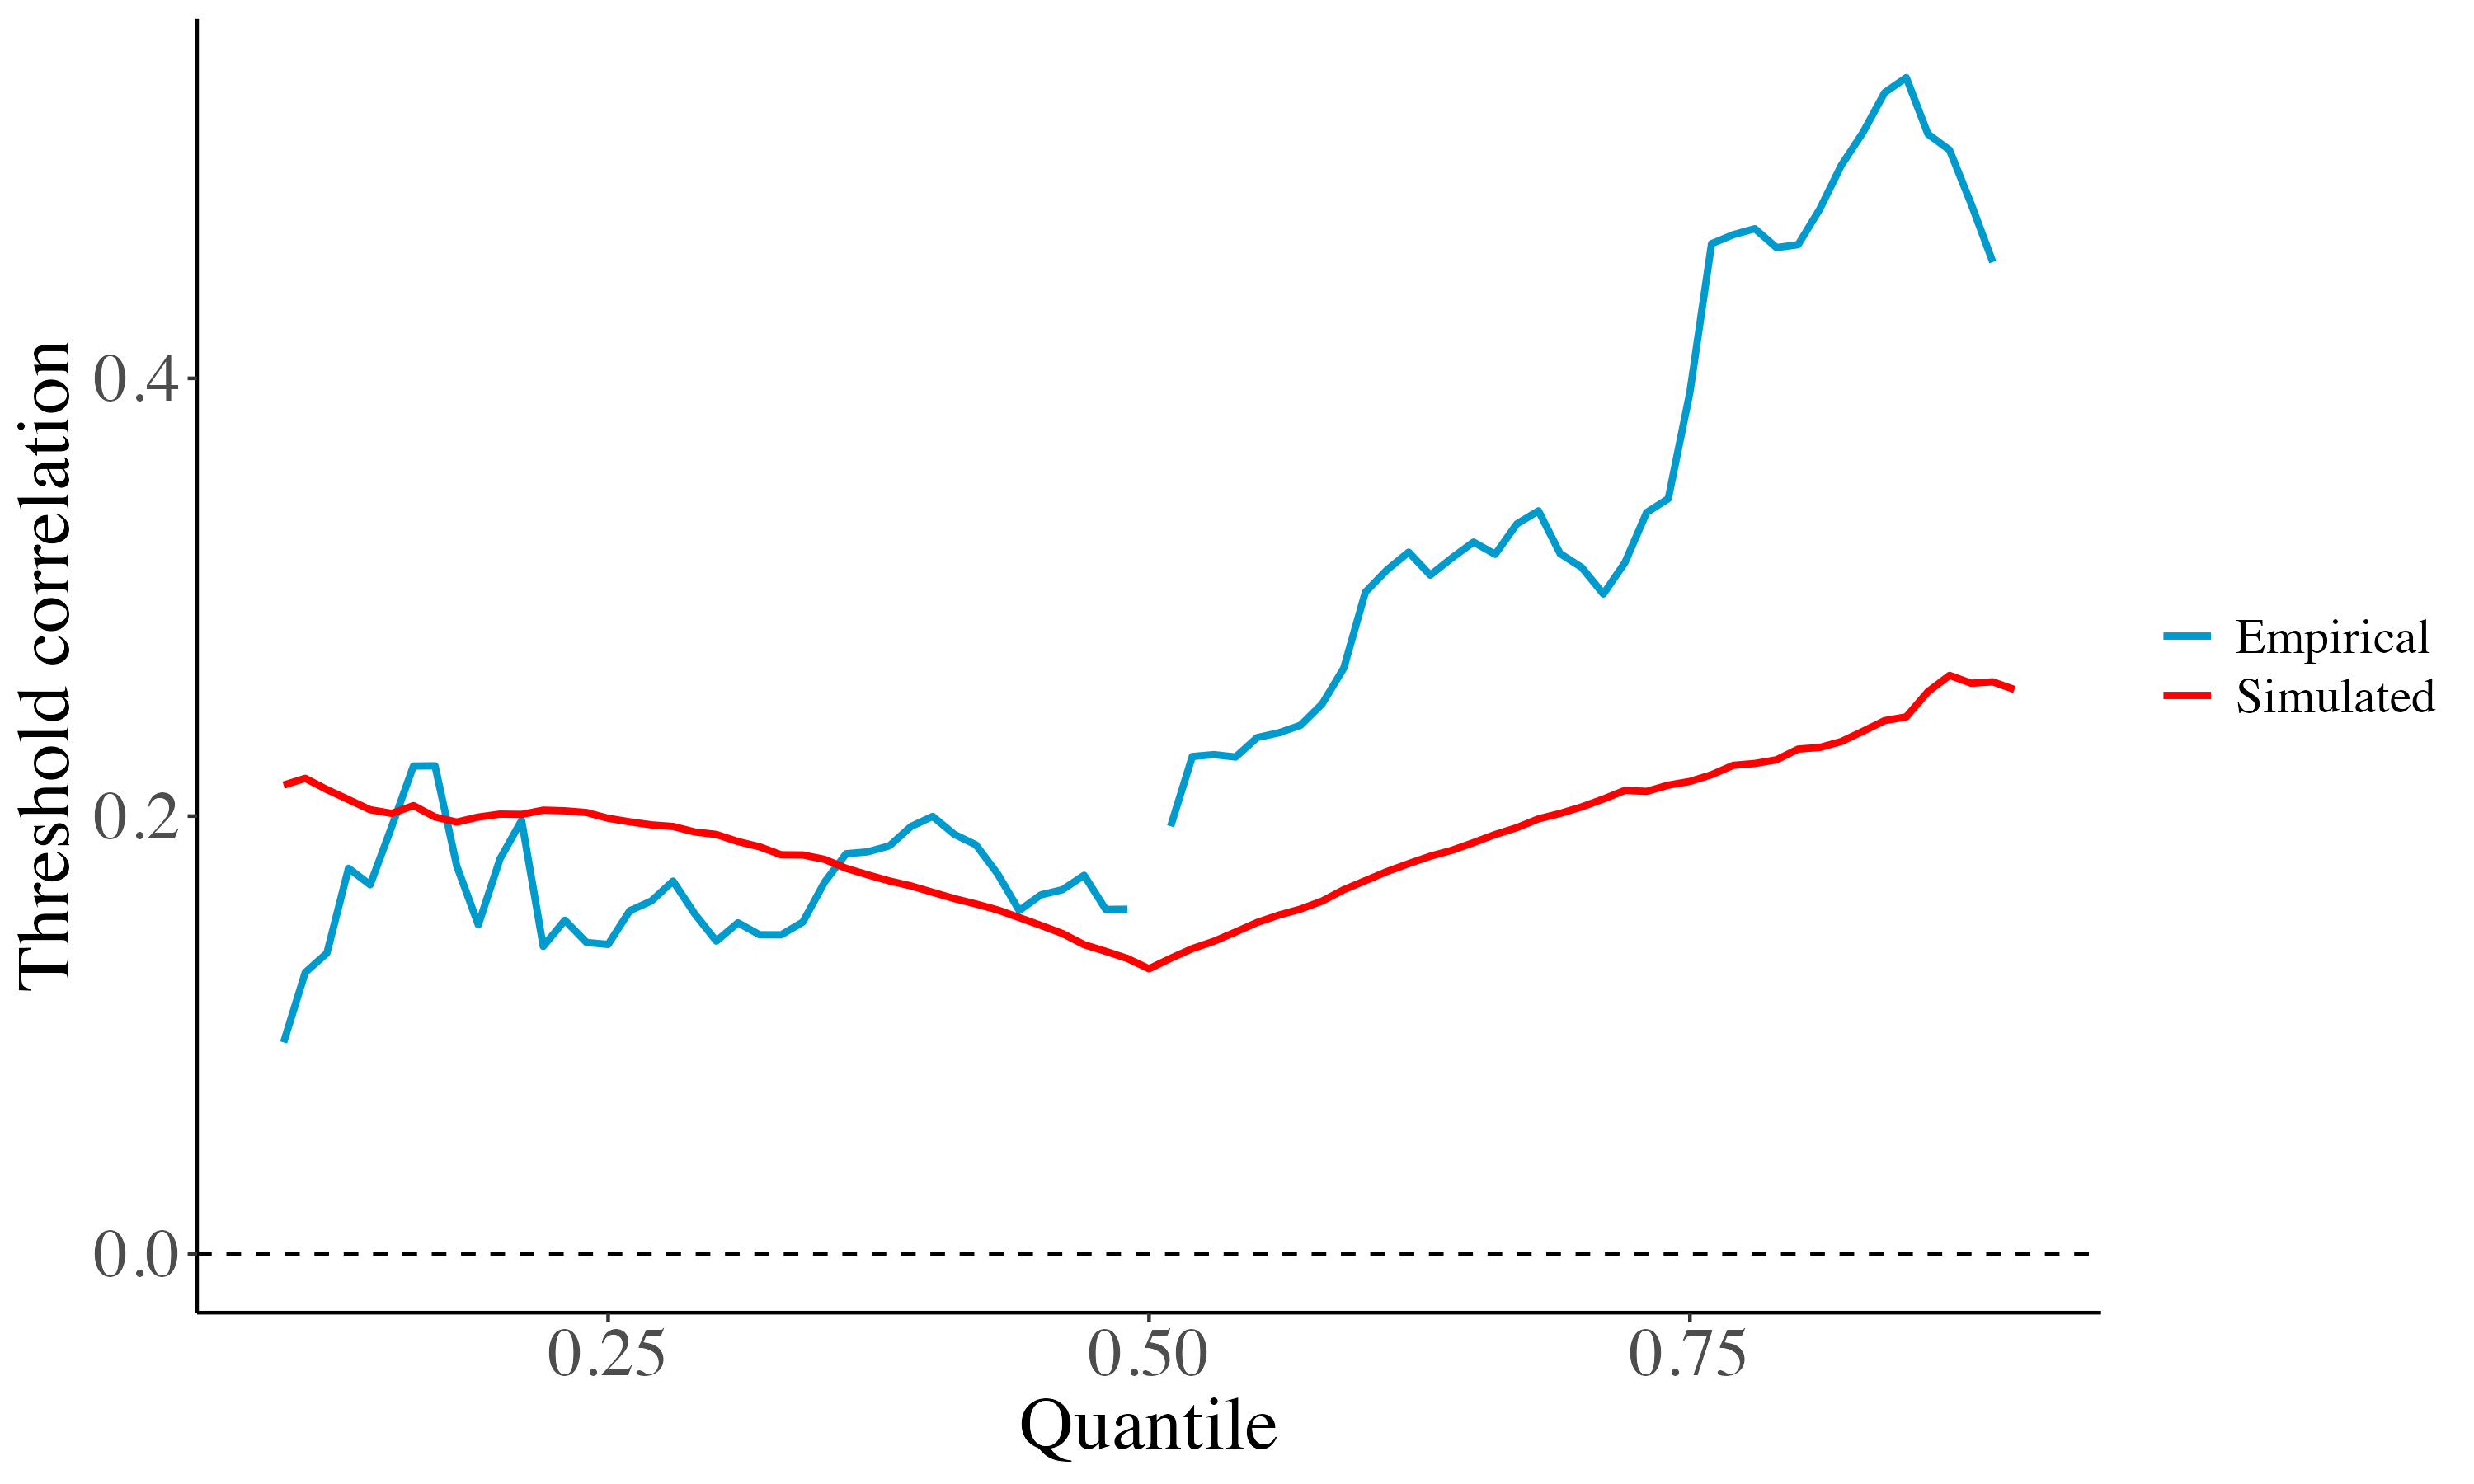
\includegraphics[scale=0.43]{../../plots/5.3.png} % Replace 
   \caption{Empirical and simulated threshold correlations of GARCH-GARCH copula.}
    \label{5.3}
\end{figure}

\begin{figure}[H]
    \centering
    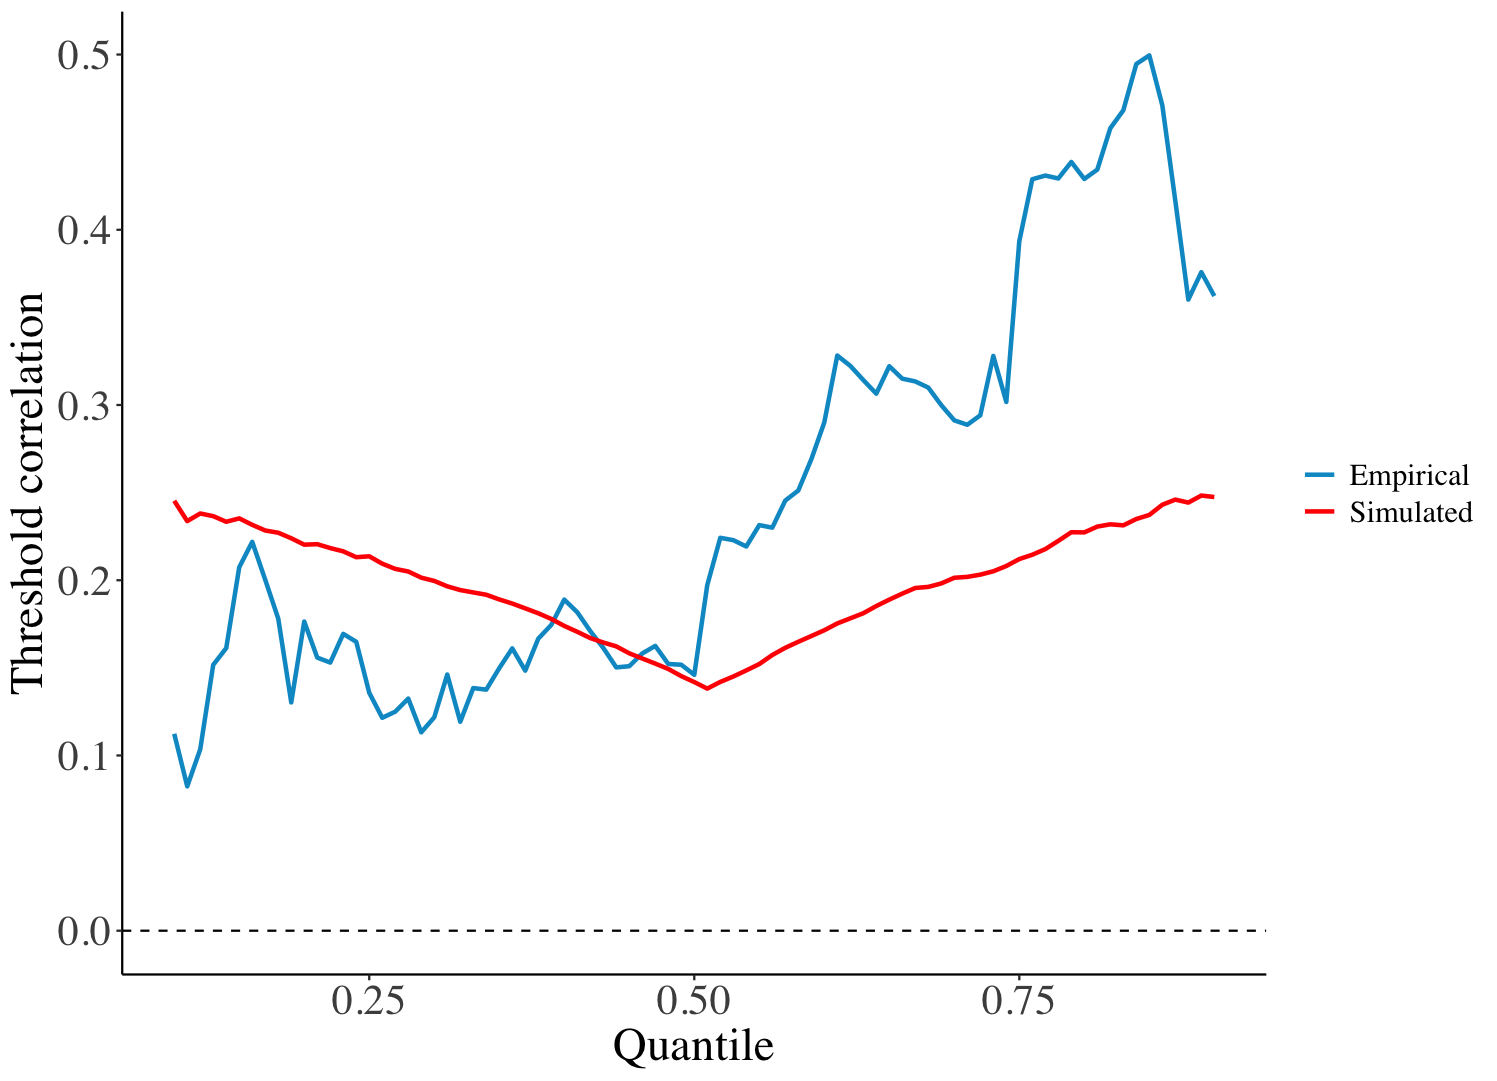
\includegraphics[scale=0.43]{../../plots/5.4.png} % Replace 
   \caption{Empirical and simulated threshold correlations of GJR-GJR copula.}
    \label{5.4}
\end{figure}

As shown by \citeA{christoffersen2011joint}, dynamic and static asymmetric copulas can match the empirical behavior of threshold correlations and thus offer a powerful alternative to the approach used in this chapter.

The subsequent step is to evaluate the forecasting performance of the copula models. Consider an equally-weighted portfolio composed of the S\&P 500 and the bond index. The validity of the multivariate copula models and their effectiveness from a risk management perspective will be assessed using this hypothetical portfolio.

Due to the complexity of the multivariate setup, closed-form expressions for the next day’s portfolio density forecast, VaR, and ES are no longer feasible. Consequently, a Monte Carlo approach is used. The algorithm is as follows:
\begin{enumerate}
\item[i.] At the end of trading day $t$, observed returns $R_{1,t}$ and $R_{2,t}$ are used to forecast the next day’s conditional volatilities $\sigma_{1,t+1}$ and $\sigma_{2,t+1}$, applying either the fitted GARCH or GJR volatility specification.
\item[ii.] Draw $M$ simulated probability pairs $(\check{u}_{1,t+1}, \check{u}_{2,t+1})$ from the fitted copula model.
\item[iii.] Transform these simulated copula probabilities into standardized shocks using the inverse of the fitted marginal distributions: $\check{z}_{i,t+1} = F_i^{-1}(\check{u}_{i,t+1}), \quad i=1,2$.
\item[iv.] Generate asset returns by scaling these shocks with the forecasted volatilities: $\check{R}_{i,t+1} = \sigma_{i,t+1} \check{z}_{i,t+1}, \quad i=1,2$.
\end{enumerate}
\newpage
After simulating $M$ scenarios of next-day returns for each asset, the corresponding portfolio returns are easily computed based on the given portfolio weights. Risk measures, including portfolio VaR and ES, can then be derived from the simulated distribution of portfolio returns. Specifically, the portfolio VaR at the 2.5\% level is estimated as the empirical 2.5th percentile of the simulated portfolio returns. Consequently, at the end of each trading day, the VaR forecast and associated simulated density of the portfolio returns can be obtained.

To further illustrate the simulation procedure, consider the case of a single asset. Figure~\ref{5.5} depicts the structure of the Monte Carlo algorithm used to simulate hypothetical next-day returns. Starting from the observed return at time $t$, the conditional variance forecast $\sigma^2_{t+1}$ is obtained using a GARCH or GJR specification. Next, draws are generated from the fitted copula to obtain simulated copula probabilities $\check{u}_{i,t+1}$, which are then transformed into shocks $\check{z}_{i,t+1}$ using the inverse of the marginal CDF. Finally, the shocks are scaled by the forecasted volatility to produce simulated returns $\check{R}_{i,t+1}$.

\begin{figure}[H]
\centering
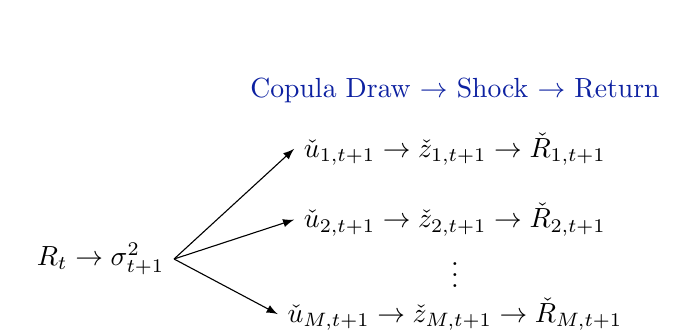
\begin{tikzpicture}[
  every node/.style={align=center},
  arrow/.style={->, >=latex},
  base/.style={minimum height=0.8cm},
  label/.style={font=\color{miAzul}},
]

% Simulation path nodes (right side)
\node[base] (z11) at (4.5,1.4) {$\check{u}_{1,t+1} \rightarrow \check{z}_{1,t+1} \rightarrow \check{R}_{1,t+1}$};
\node[base] (z21) at (4.5,0.5) {$\check{u}_{2,t+1} \rightarrow \check{z}_{2,t+1} \rightarrow \check{R}_{2,t+1}$};
\node[base] (dots1) at (4.5,-0.1) {$\vdots$};
\node[base] (zmc1) at (4.5,-0.7) {$\check{u}_{M,t+1} \rightarrow \check{z}_{M,t+1} \rightarrow \check{R}_{M,t+1}$};

% Root node centered
\node[base] (sigma) at (0,0) {$R_t \rightarrow \sigma^2_{t+1}$};

% Arrows from root to paths
\draw[arrow] (sigma.east) -- (z11.west);
\draw[arrow] (sigma.east) -- (z21.west);
\draw[arrow] (sigma.east) -- (zmc1.west);

% Label above the top simulation arrow (closer)
\node[label, above=0.05cm of z11] {Copula Draw $\rightarrow$ Shock $\rightarrow$ Return};

\end{tikzpicture}
\caption{Simulation algorithm structure for next day's return.}
\label{5.5}
\end{figure}
\newpage
Once the density forecast and VaR for day $t+1$ have been generated, the accuracy of the copula-based model can be evaluated. This is done by comparing the realized return $R_{t+1}$ to the simulated distribution, analogous to a Probability Integral Transform (PIT) based now on the Monte Carlo density. The model’s effectiveness in risk management is assessed using VaR validation techniques similar to those applied in \hyperref[chap:4]{Chapter 4}.

Figures \ref{5.6} and \ref{5.7} display the 2.5\% portfolio VaR along with the breaches observed during the test period. The breaches are almost identical across the two copula models, with the primary weakness again being the lack of independence between violations. Additionally, observe that the GJR-GJR copula model produces sharper increases in VaR following negative returns—reflecting its volatility specification—and thus adapts more quickly, though still not rapidly enough to capture the large negative returns at the onset of President Trump’s tariffs. Table \ref{5.3} summarizes the results of the Christoffersen tests for these models. From a risk management perspective, both copula models may offer an acceptable coverage, but are incapable to adapting quickly to drastic changes in the volatility regime. 

\begin{figure}[H]
    \centering
    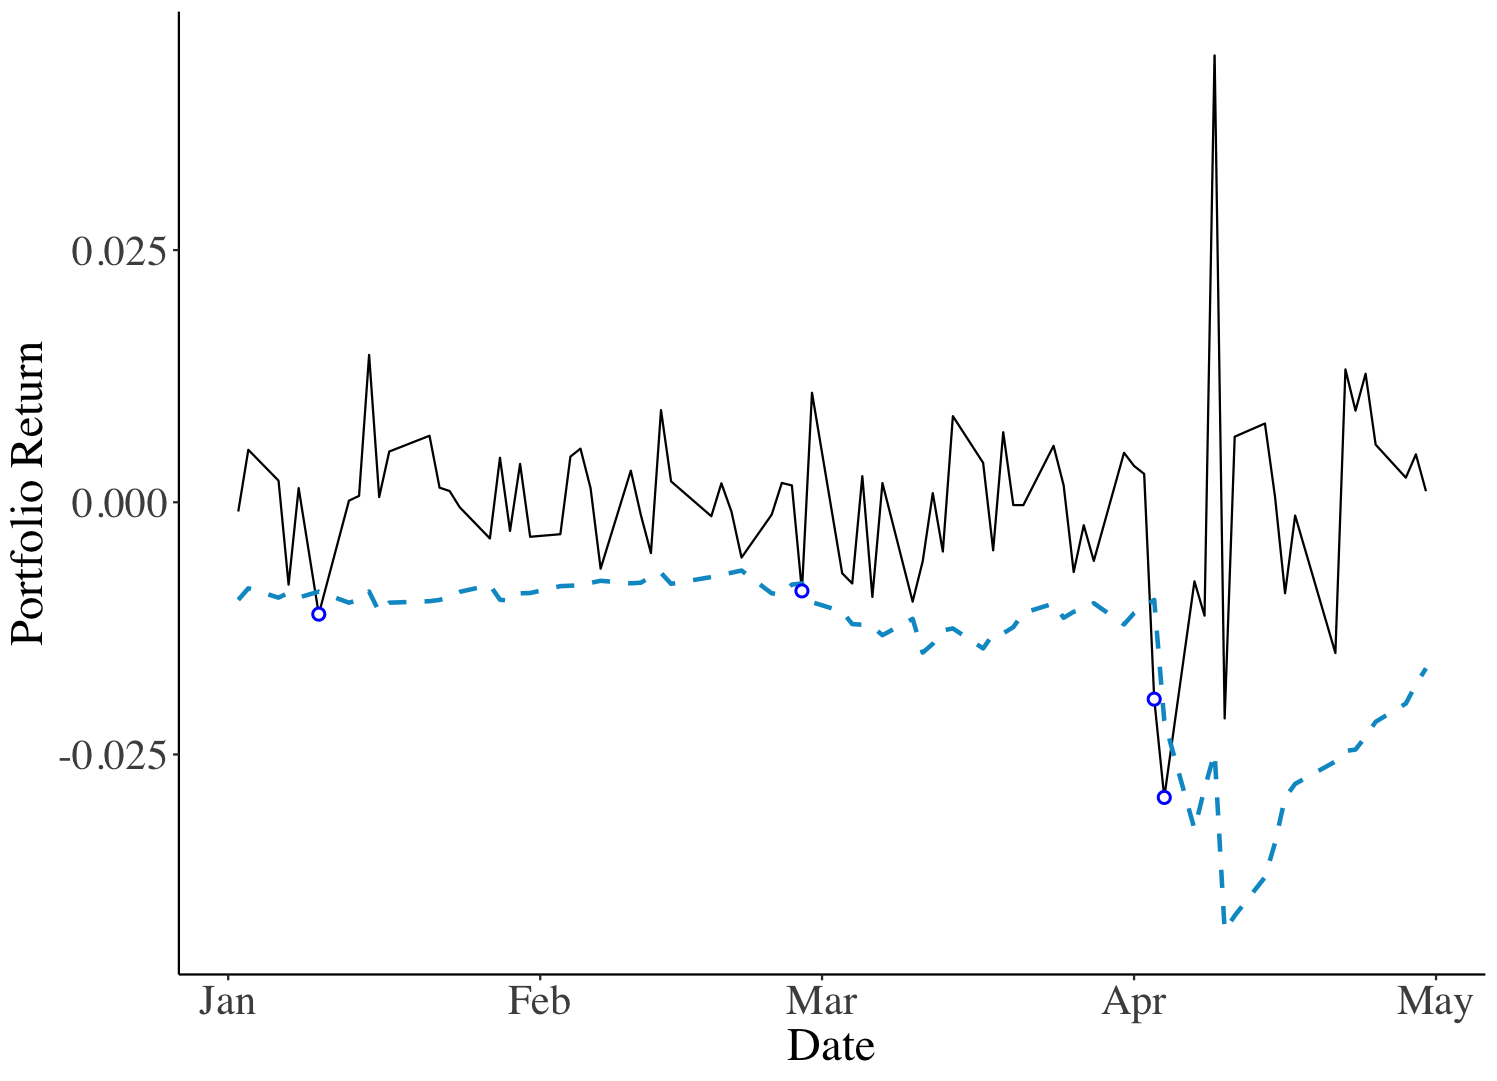
\includegraphics[scale=0.18]{../../plots/5.6.png} % Replace 
   \caption{2.5\% VaR breaches, GARCH-GACRH Copula.}
    \label{5.6}
\end{figure}

\begin{figure}[H]
    \centering
    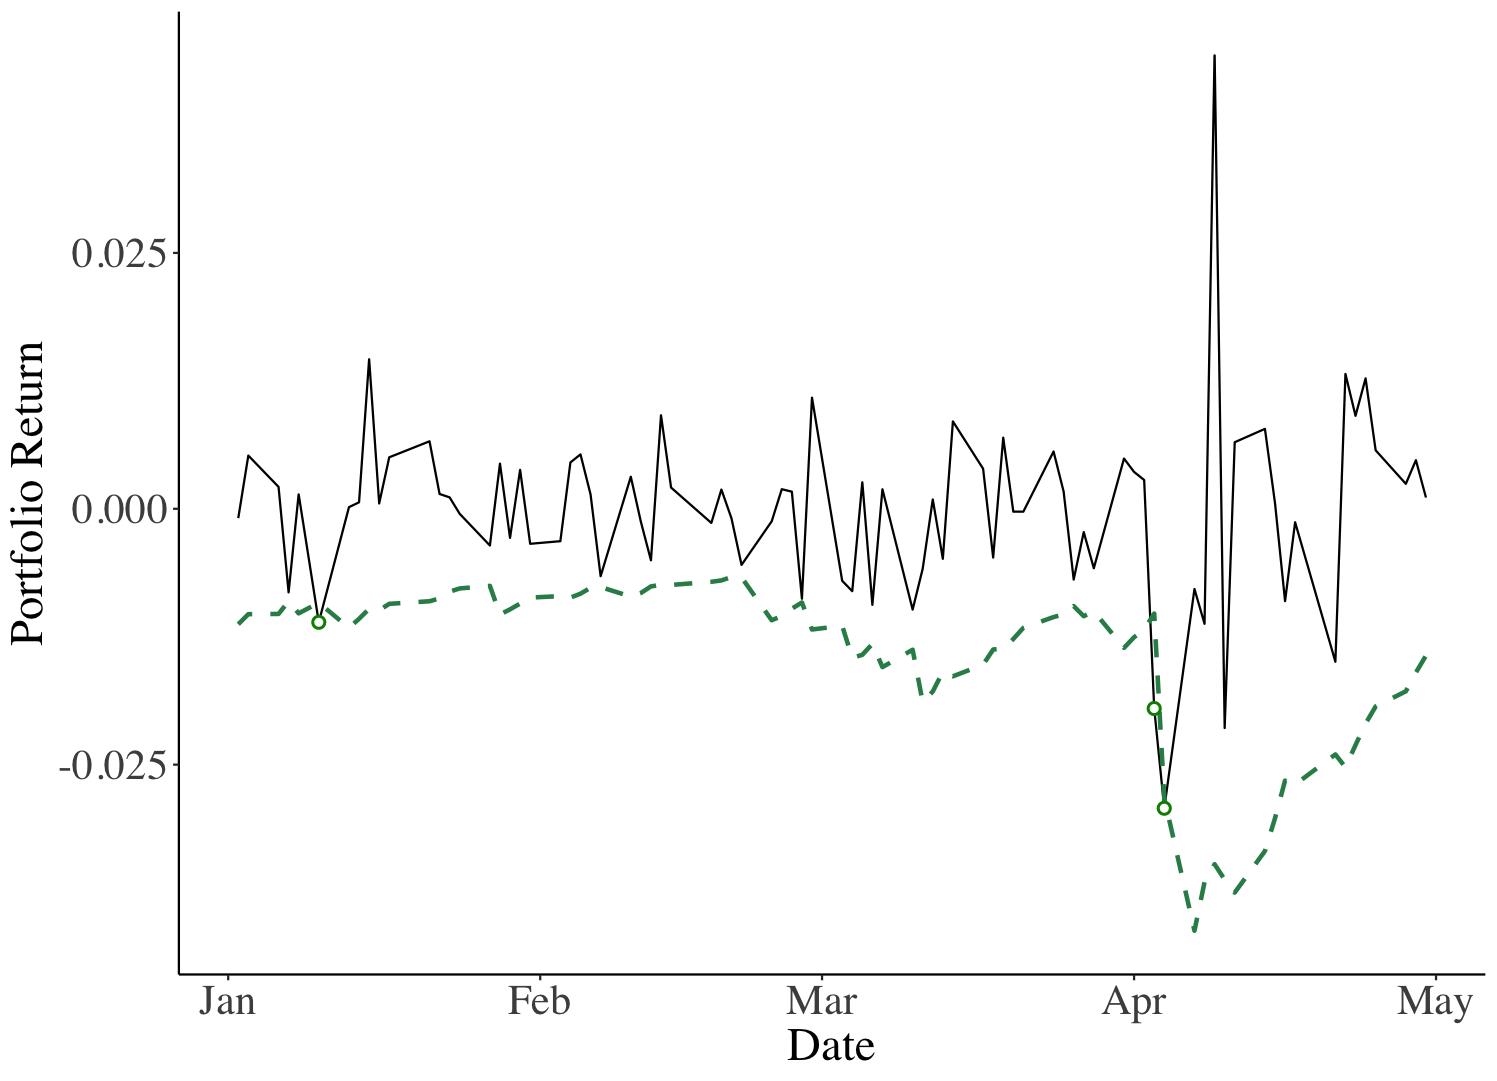
\includegraphics[scale=0.18]{../../plots/5.7.png} % Replace 
   \caption{2.5\% VaR breaches, GJR-GJR Copula.}
    \label{5.7}
\end{figure}

\begin{table}[htbp]
\centering
\begin{tabular}{llcc}
\toprule
\textbf{Test} & \textbf{p-value} & \textbf{GARCH-GARCH} & \textbf{GJR-GJR} \\
\midrule
$LR_{\text{uc}}$   & Theoretical & 0.2138 &  0.5168 \\
                   & Simulated   & 0.188 &  0.554 \\
$LR_{\text{ind}}$  & Theoretical & 0.1582 & 0.0729 \\
                   & Simulated   & 0.03 & 0.013 \\
$LR_{\text{cc}}$   & Theoretical & 0.1706 & 0.1622 \\
                   & Simulated   &  0.217 & 0.2 \\
\bottomrule
\end{tabular}
\caption{Theoretical and simulated $p$-values for VaR testing statistics.}
\label{tab:5.3}
\end{table}

Next, the statistical validity of the copula models is evaluated by examining the portfolio PIT histograms presented in Figures \ref{5.8} and \ref{5.9}. No significant deviations from uniformity are apparent. Performing a Kolmogorov–Smirnov test on the normally transformed PIT values, following the procedure described in \hyperref[chap:4]{Chapter4}, yields $p$-values of 0.5271 for the GARCH-GARCH model and 0.4872 for the GJR-GJR model. These results suggest that the Monte Carlo-generated densities constitute valid density forecasts for the portfolio returns. Figures \ref{5.10} and \ref{5.11} further illustrate the validity by comparing the empirical CDFs of the normally transformed PIT values against the theoretical standard normal CDF, highlighting the K-S test statistic.

\begin{figure}[H]
    \centering
    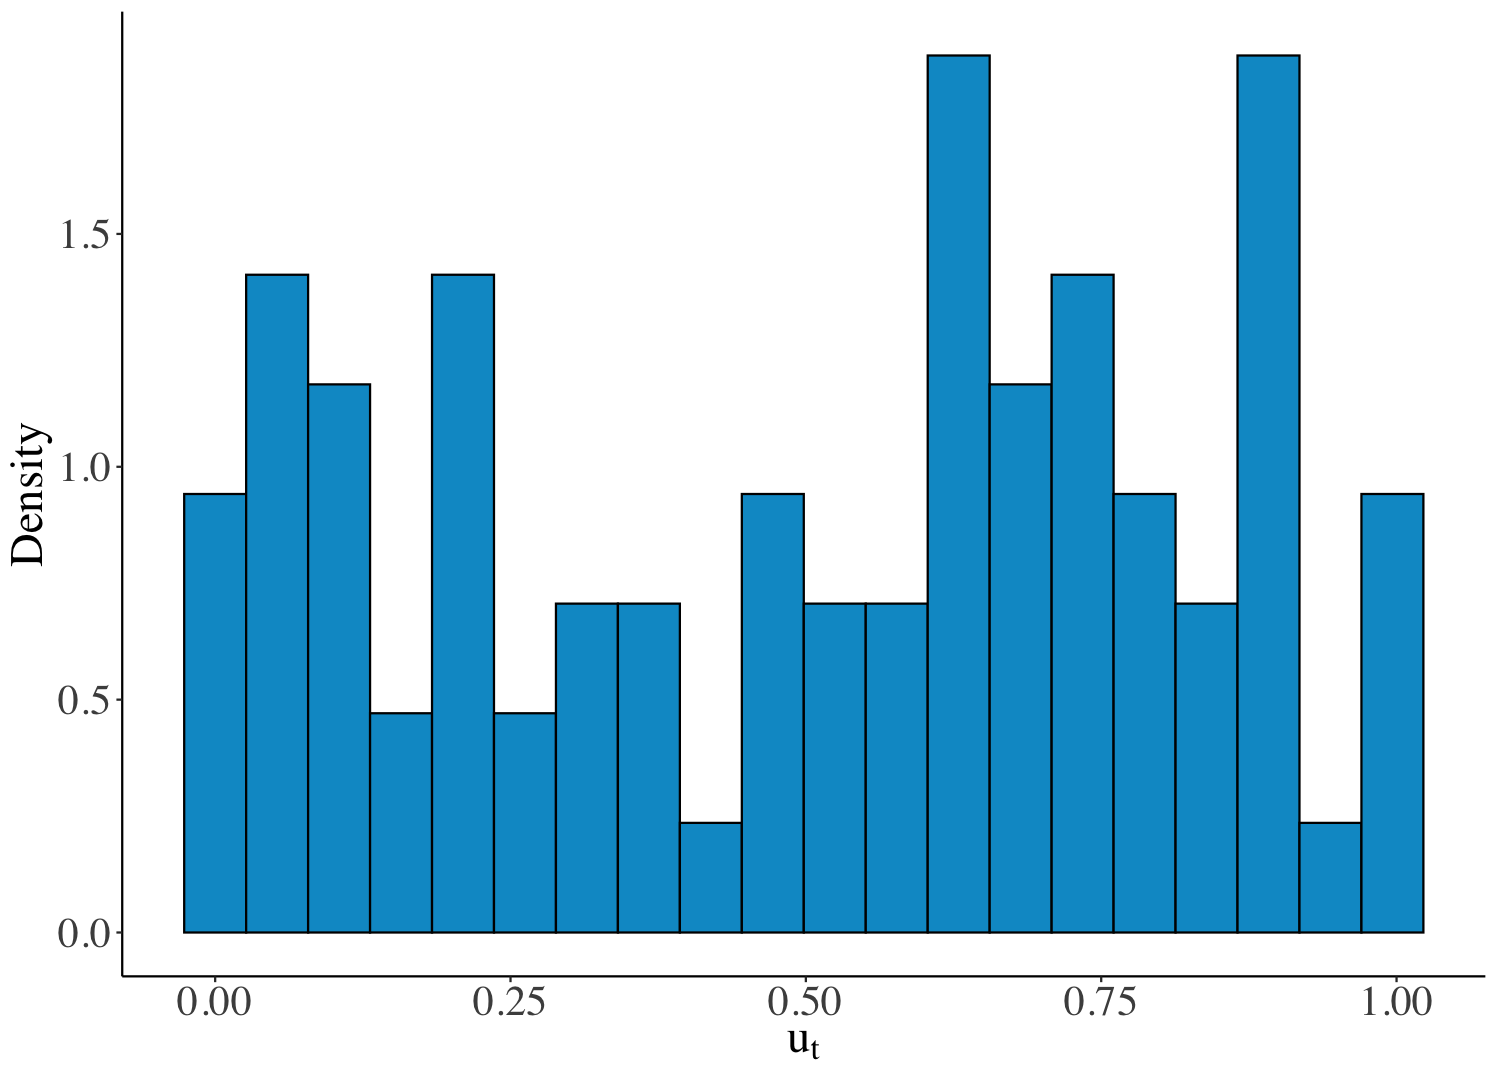
\includegraphics[scale=0.18]{../../plots/5.8.png} % Replace 
   \caption{Histogram of PIT values, GARCH-GARCH copula.}
    \label{5.8}
\end{figure}

\begin{figure}[H]
    \centering
    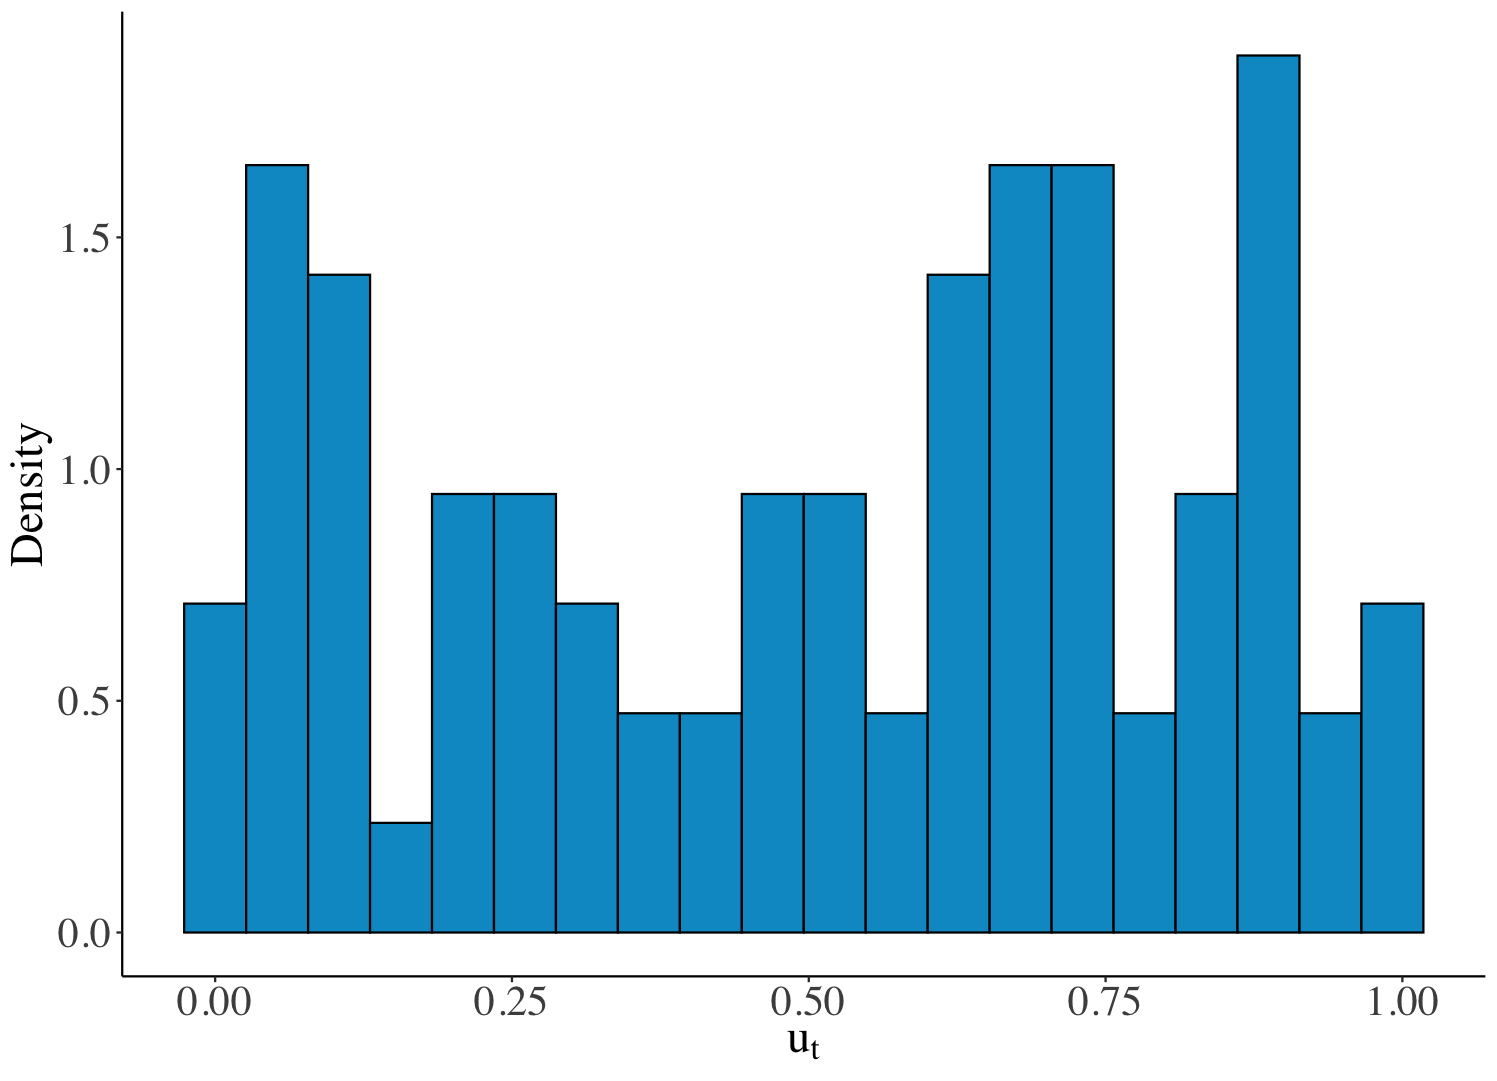
\includegraphics[scale=0.18]{../../plots/5.9.png} % Replace 
   \caption{Histogram of PIT values, GJR-GJR copula.}
    \label{5.9}
\end{figure}

\begin{figure}[H]
    \centering
    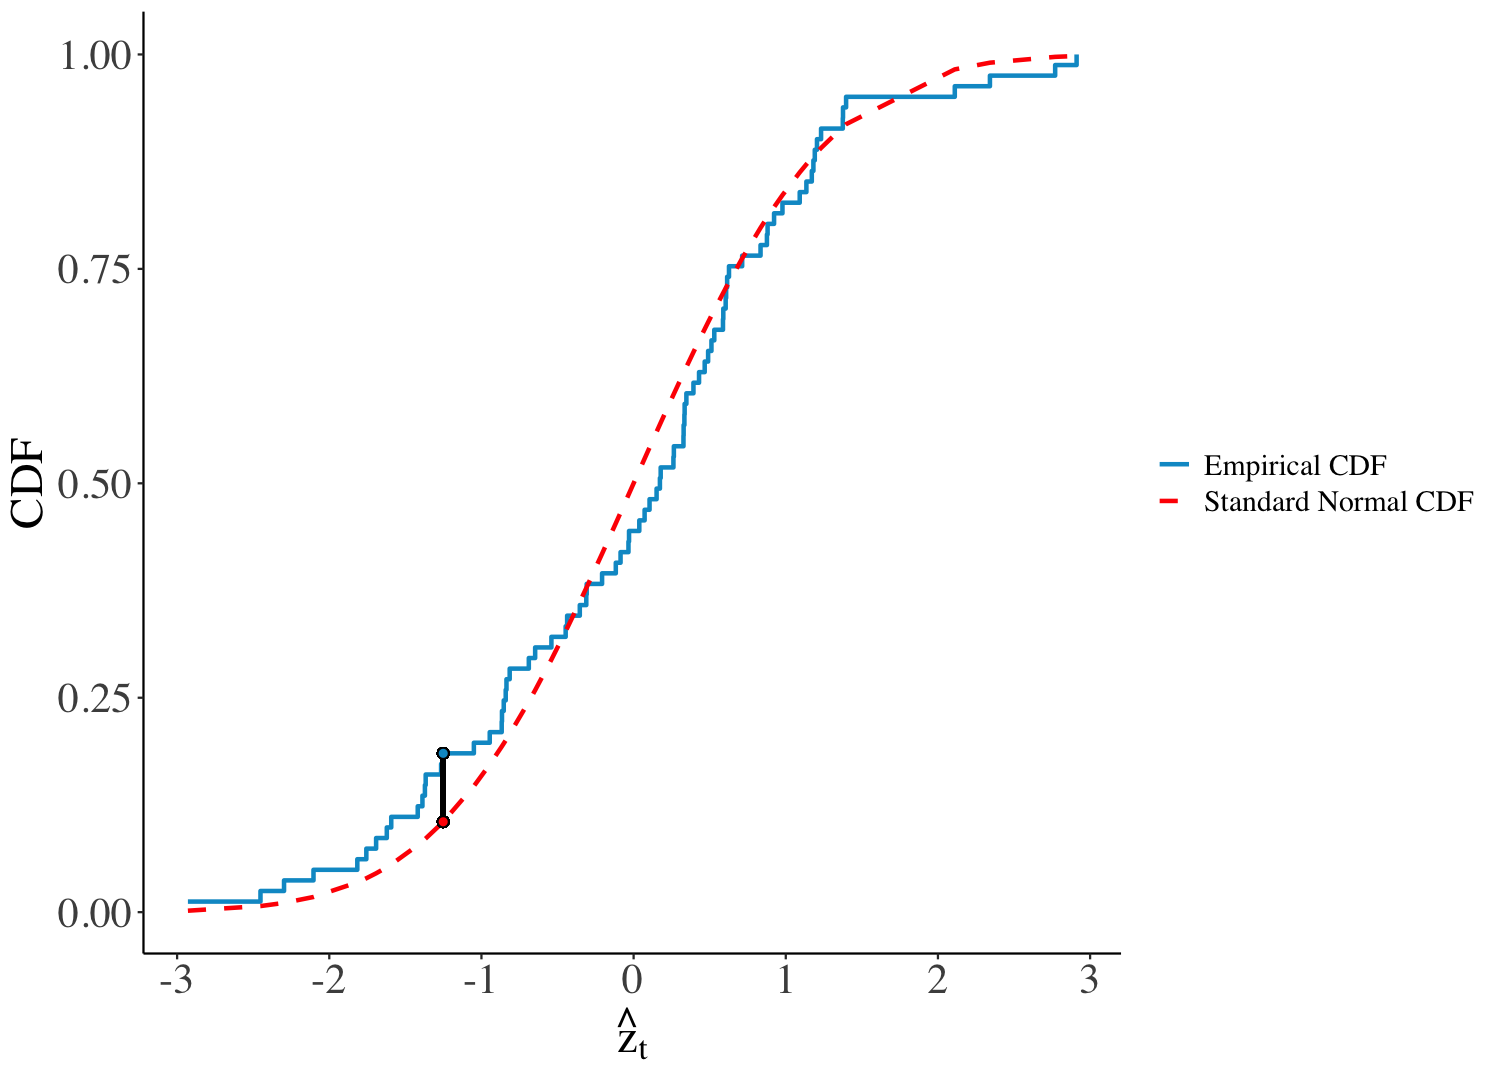
\includegraphics[scale=0.18]{../../plots/5.10.png} % Replace 
   \caption{Kolmogorov-Smirnov test on $\hat{z}_{t+1}$, GARCH-GARCH copula}
    \label{5.10}
\end{figure}

\begin{figure}[H]
    \centering
    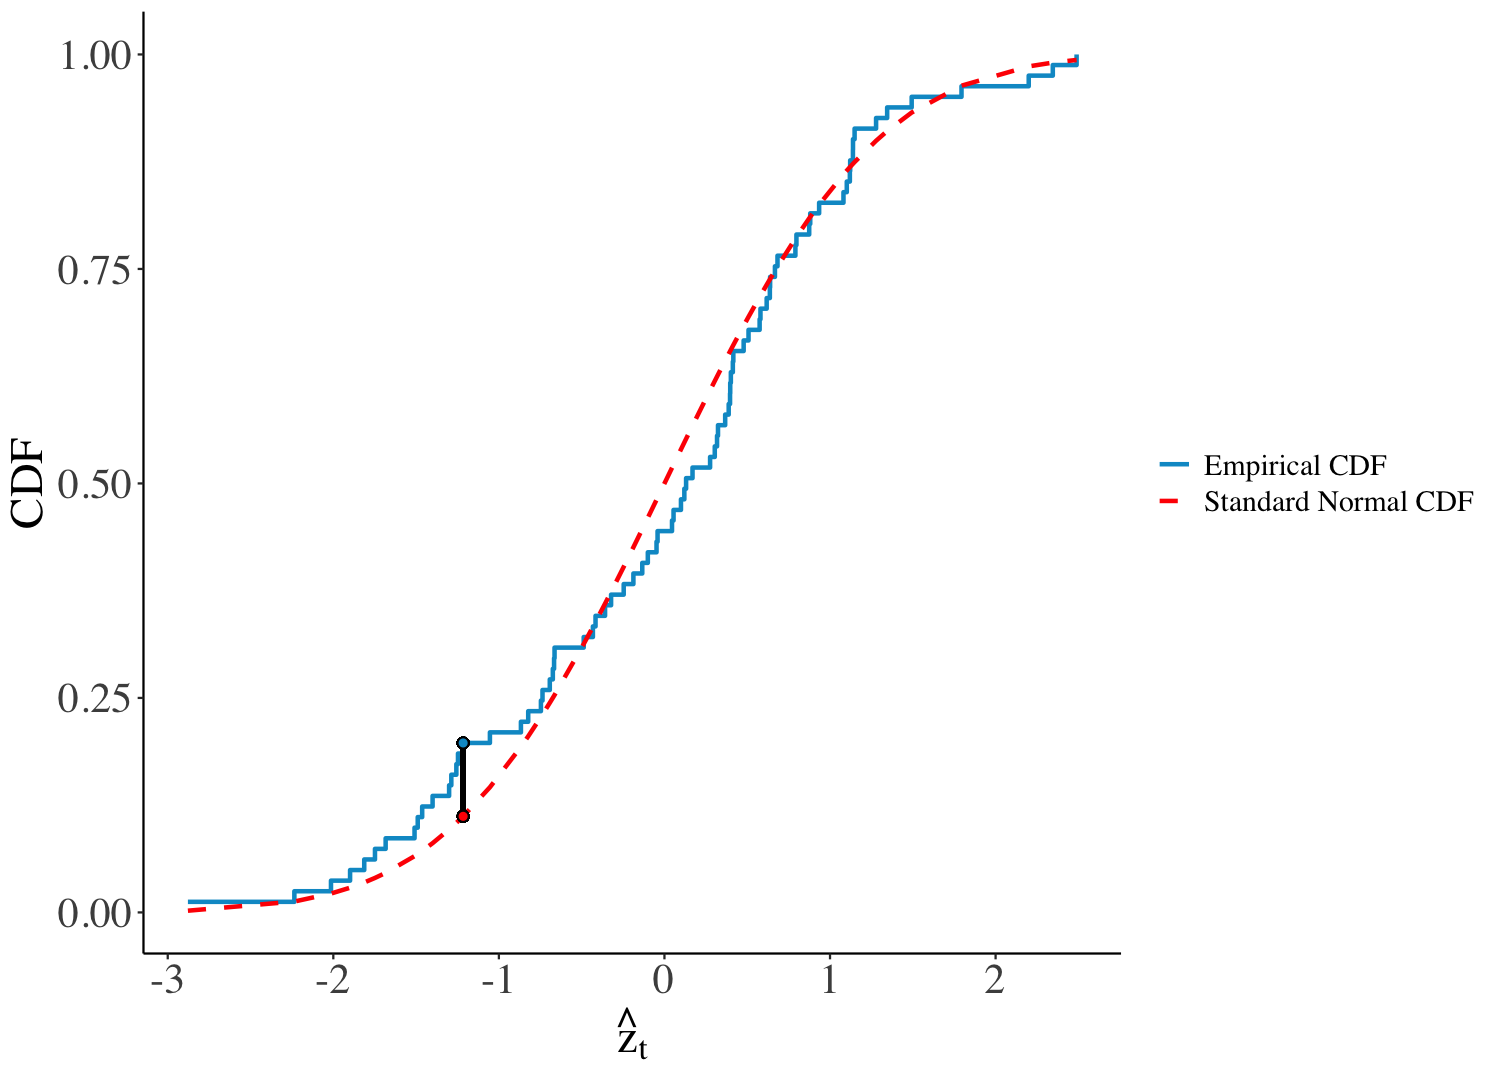
\includegraphics[scale=0.18]{../../plots/5.11.png} % Replace 
   \caption{Kolmogorov-Smirnov test on $\hat{z}_{t+1}$, GJR-GJR copula}
    \label{5.11}
\end{figure}

To conclude, copula models offer two main advantages. First, they allow univariate models for individual asset returns to be estimated independently, leveraging a wide and accessible body of literature. This flexibility makes complex univariate modeling more manageable. Second, copula models effectively capture nonlinear dependencies between asset returns, which are especially important from a risk management perspective. At the same time, the approach considered in this chapter has important limitations. The static symmetric $t$-copula is unable to capture the time variation in cross-asset dependence documented earlier, and its symmetry prevents it from fully reproducing the asymmetric tail dependence suggested by the threshold correlation plots. Moreover, the resulting VaR forecasts still adapt too slowly to abrupt changes in volatility. Thus, while the copula framework represents a practical and powerful approach to multivariate modeling, more flexible dynamic and asymmetric copula specifications appear necessary for a fuller description of the dependence between financial assets.

\newpage
\newpage
\chapter*{Conclusion}
\addcontentsline{toc}{chapter}{Conclusion}

This thesis set out to provide a comprehensive, step-by-step framework for modeling financial returns, beginning with univariate modeling techniques and culminating in a multivariate risk-modeling approach based on copulas. Each chapter built on the previous one, combining theoretical underpinnings with practical implementation for key models in financial econometrics.

\hyperref[chap:1]{Chapter 1} introduced the empirical features of asset returns and framed the modeling challenge. It also described the dataset used throughout: daily returns for the S\&P~500 and a 10-year U.S.\ Treasury note index (Bloomberg ticker: SPBDU1BT Index), with a training sample from January~2015 to December~2024 and a forecasting (test) sample from January~2025 to April~2025.

\hyperref[chap:2]{Chapter 2} addressed the first challenge—modeling dynamic volatility—via GARCH(1,1) and GJR–GARCH(1,1). \hyperref[chap:3]{Chapter 3} turned to the parametric modeling of shocks, considering an asymmetric Student’s $t$-distribution and a peak-over-threshold approach from extreme value theory (EVT).

\hyperref[chap:4]{Chapter 4} evaluated model validity and usefulness for risk management. The chosen GARCH specifications captured the conditional volatility structure, and density-forecast diagnostics suggested statistical adequacy in samples. For risk forecasts, however, models based on the asymmetric $t$-distribution failed to achieve acceptable Value-at-Risk (VaR) coverage and independence of violations, while EVT-based models achieved more acceptable coverage but did not pass independence tests.

\hyperref[chap:5]{Chapter 5} proposed a multivariate framework based on a symmetric $t$-copula to capture threshold correlations while, for tractability, abstracting from time variation in dependence. In the test set, this static copula struggled with sudden increases in volatility and, consequently, with independence of VaR violations. Nonetheless, PIT-based diagnostics—histograms and Kolmogorov–Smirnov tests on the normal transform—indicated that the copula-based portfolio density forecasts were statistically well calibrated, supporting their validity as density forecasts. Together with the VaR shortcomings noted above, these findings motivate the broader appraisal of the framework's limitations that follows.

Several limitations should temper the conclusions drawn from this work. First, the empirical scope is deliberately narrow: a bivariate portfolio of the S\&P~500 and a 10-year U.S.\ Treasury index, evaluated on a four-month out-of-sample window (January--April 2025) that, while informative as a stress episode, yields too few violations for high-power backtests and spans only one regime shift. Second, all models are fit once on the full 2014--2024 sample rather than re-estimated through rolling or expanding windows, so the parameters reflect a predominantly low-rate, equity-bull period and may adapt sluggishly to structural breaks. Third, the GARCH(1,1) and GJR--GARCH(1,1) specifications inherit well-known caveats---fixed lag order, near-integrated persistence that complicates long-horizon variance forecasts, and reliance on squared returns as a noisy proxy for conditional variance---while the EVT and asymmetric-t shock models assume time-invariant tail parameters. Finally, the risk analysis is conducted on a hypothetical, equally weighted, buy-and-hold position, abstracting from transaction costs, rebalancing, and liquidity effects that any practical implementation would face. These limitations do not invalidate the framework, but they delimit the conditions under which its forecasts can be trusted; addressing them points to hybrid specifications that pair the conservative tail treatment of EVT with shock processes that admit time-varying skewness and kurtosis, and to asymmetric or dynamic copula families for the multivariate layer.

Throughout the thesis, emphasis was placed on balancing theoretical
clarity with empirical rigor. Modeling choices were always accompanied
by justification, comparisons with alternatives, and diagnostic tools
to evaluate performance. The methodologies were implemented and illustrated using real financial data, with all \Rlogo\ code made openly available in the accompanying \href{https://github.com/ferpmillan/thesis}{GitHub repository} to promote full
reproducibility.

Ultimately, the structured modeling path presented here not only equips
readers with robust and practical tools to approach financial return
modeling, but also underscores the ongoing relevance and vitality of
questions first posed decades ago—questions that continue to drive
innovation and deepen our understanding of financial markets.
\cleardoublepage
\backmatter
\bibliography{\thesisbib}
\end{document}
